\documentclass[13pt]{article}

\usepackage{amsmath,amsthm,amssymb}
%%%%% Matrix stretcher
% use it as:
%\begin{pmatrix}[1.5]
% ...
\makeatletter
\renewcommand*\env@matrix[1][\arraystretch]{%
  \edef\arraystretch{#1}%
  \hskip -\arraycolsep
  \let\@ifnextchar\new@ifnextchar
  \array{*\c@MaxMatrixCols c}}
\makeatother
%%%%%%%%%%%%%%%%%%%%%%%%%%
\newcommand\extrafootertext[1]{%
    \bgroup
    \renewcommand\thefootnote{\fnsymbol{footnote}}%
    \renewcommand\thempfootnote{\fnsymbol{mpfootnote}}%
    \footnotetext[0]{#1}%
    \egroup
}


% Colors
\usepackage[dvipsnames]{xcolor}

\definecolor{C0}{HTML}{1d1d1d}
\definecolor{C1}{HTML}{1e3668}
\definecolor{C2}{HTML}{199d8b}
\definecolor{C3}{HTML}{d52f4c}
\definecolor{C4}{HTML}{5ab2d6}
\definecolor{C5}{HTML}{ffb268}
\definecolor{C6}{HTML}{ff7300} % for commenting - {fire orange}dd571c
\definecolor{C7}{HTML}{777b7e} % for remarks - {steel grey}
\color{C0}
%
% fonts
\usepackage[no-math]{fontspec}

\emergencystretch=8pt
\hyphenpenalty=1000 % default 50
\tolerance=800      % default 200
%\righthyphenmin=4
%\lefthyphenmin=4

\setmainfont[
    BoldFont = Vollkorn-Bold,
    ItalicFont = Vollkorn-Italic,
    BoldItalicFont={Vollkorn-BoldItalic},
    RawFeature=+lnum,
]{Vollkorn}
\usepackage[scale=.78]{luatexja-fontspec}
\setmainjfont{BabelStone Han}[AutoFakeBold]

% This package simplifies the insertion of external multi-page PDF or PS doc- uments.
\usepackage{pdfpages}

% cref
\usepackage{hyperref}
\hypersetup{
    colorlinks=true,
    linkcolor=C4,
    filecolor=magenta,      
    urlcolor=cyan,
    }

\usepackage[nameinlink,noabbrev,capitalize]{cleveref}
% \crefname{ineq}{}{}
% \crefname{equation}{}{}
% \creflabelformat{ineq}{#2{\textup{(1)}}#3}
% \creflabelformat{equation}{#2\textup{(#1)}#3}

% theorem-like environment
\newtheorem{theorem}{Theorem}[section]
\newtheorem{assumption}[theorem]{Assumption}
\newtheorem{lemma}[theorem]{Lemma}
\newtheorem{corollary}[theorem]{Corollary}
\newtheorem{proposition}[theorem]{Proposition}
\newtheorem{property}[theorem]{Property}

\newtheorem{definition}[theorem]{Definition}
\newtheorem{notation}[theorem]{Notation}

\theoremstyle{definition}
\newtheorem{example}[theorem]{Example}
\newtheorem{problem}[theorem]{Problem}

% framed package is great
\usepackage{framed}
\newenvironment{solution}
{\color{C2}\begin{framed}\begingroup\textbf{Solution:} }
  {\endgroup\end{framed}}

\newtheoremstyle{remark}% name of the style to be used
  {}% measure of space to leave above the theorem. E.g.: 3pt
  {}% measure of space to leave below the theorem. E.g.: 3pt
  {\color{C3}}% name of font to use in the body of the theorem
  {}% measure of space to indent
  {\color{C3}\bfseries}% name of head font
  {.}% punctuation between head and body
  { }% space after theorem head; " " = normal interword space
  {}
\theoremstyle{remark}
\newtheorem{remarkx}[theorem]{Remark}
\newenvironment{remark}
  {\pushQED{\qed}\renewcommand{\qedsymbol}{$\triangle$}\remarkx}
  {\popQED\endremarkx}
  
\newenvironment{point}
  {\O~~}
  {}

\usepackage{thmtools}
\usepackage{thm-restate}




% Page Formatting
\usepackage[
    paper=b5paper,
    inner=22mm,         % Inner margin
    outer=22mm,         % Outer margin
    bindingoffset=0mm, % Binding offset
    top=28mm,           % Top margin
    bottom=22mm,        % Bottom margin
    %showframe,         % show how the type block is set on the page
]{geometry}

\setlength{\parindent}{0em}
\setlength{\parskip}{.7em}


\usepackage{tikz}
\usepackage{graphicx}
\usepackage{enumitem}
\setlist{topsep=0pt}

\usepackage{bm}

\usepackage[font=scriptsize,labelfont=bf]{caption}
\usepackage{listings}
\lstset{basicstyle=\ttfamily,breaklines=true}
% \setlength{\parskip}{1em}
% \setlength{\parindent}{0em}
\usepackage{dsfont}
\newcommand{\bOne}{\mathds{1}}
\newcommand{\PP}{\mathbb{\mathbf{P}}}
\newcommand{\EE}{\mathbb{E}}
\newcommand{\VV}{\mathbb{\mathbf{V}}}
\newcommand{\CoV}{\operatorname{Co\mathbb{\mathbf{V}}}}

% header
\usepackage{fancyhdr}
\pagestyle{fancy}
\fancyhead{}
\fancyhead[L]{\small   \bfseries Honors Paper}
\fancyhead[C]{\small   \bfseries Spring 2023}
\fancyhead[R]{\small   \bfseries Zhou}


\begin{document}

\begin{center}
    \text{\Large{Mean-Variance Optimization and Beyond
}}
    
    {\text{Kaiwen Zhou}}


\end{center}

\tableofcontents
\newpage
\vspace{2em}


\section{Introduction}

This research paper is a study I've conducted on various portfolio allocation topics. It begins with an exploration of the classical mean-variance optimization framework and its derivatives, such as the CAPM theory and Arbitrage Pricing Theory. The study then delves into several models designed to address the limitations of the classical mean-variance optimization framework, including the Black-Litterman model.

The discussion continues with the Black-Litterman-APT model, which proposes a kind of `systematic' trading strategy. This model counters the drawback of the classical Black-Litterman framework which relies heavily on personal perception and views of the market, thereby limiting the number of assets an investor can incorporate into their portfolio. After all, it's impossible for one person to have insightful knowledge about every stock in the market unless they are the market themselves. This model's origin can be traced back to paper \cite{kolm2017}.

Finally, we introduce the framework proposed by Attilio Meucci, which, in my view, is an excellent model. His insights on market invariants are enlightening, and his framework offers a structured way of making investment decisions compatible with all asset classes and various popular strategies in the field.

To bridge theory and practice, we conduct an empirical analysis comparing various models, frameworks, and techniques that we have presented and analyzed. We conclude our research with a discussion on future potential improvements to refine our current model.

This research paper should reflect my learning journey and my evolving understanding of the topics discussed. I would like to extend my heartfelt gratitude to Prof. Jonathan Goodman, whose guidance and book recommendations have significantly enriched my research experience. Indeed, there is no greater joy than having the wisdom of a mentor lighting the path of inquiry. Thanks.

\newpage
\section{Preliminaries}
In this section, we introduce several preliminaries that would be essential for our research.


%%%%%%%%%%%%%%%%%%%%%%%%%%%%%%%%%%%%%%

\subsection{Karush–Kuhn–Tucker (KKT) conditions}\label{sec:Karush–Kuhn–Tucker (KKT) conditions}
{\color{C6} The KKT conditions are the first-order necessary conditions for a non-linear constrained optimization problem.}
\subsubsection{Problem Formulation}
Consider the following nonlinear minimization / maximization problem:
\begin{problem}
    \textbf{(Target Nonlinear Optimization Problem)} $$
\begin{aligned}
 \text { optimize } \qquad &f(\bm{x}) \\
 \text { subject to } \qquad &g_i(\bm{x}) \leq 0, i=1, \ldots, m\\
&h_j(\bm{x})=0, j=1, \ldots, \ell.
\end{aligned}
$$
where 
\begin{itemize}
    \item $\bm{x} \in \mathbf{X}$ is the optimization variable chosen from a convex subset of $\mathbb{R}^n$.
    \item $f: \mathbb{R}^n \rightarrow \mathbb{R}$ is the objective function.
    \item $g_i: \mathbb{R}^n \rightarrow \mathbb{R} (i=1, \ldots, m)$ are the inequality constraint functions and have subderivatives at a point $x^* \in \mathbb{R}^n$..
    \item $h_j: \mathbb{R}^n \rightarrow \mathbb{R} (j=1, \ldots, \ell)$ are the equality constraint functions and have subderivatives at a point $x^* \in \mathbb{R}^n$.
\end{itemize}
\end{problem}

\subsubsection{Corresponding Lagrangian}
Corresponding to the constrained optimization problem one can form the Lagrangian function
$$
\mathcal{L}(\bm{x}, \mu, \lambda)=f(\bm{x})+\mu^{\top} \mathbf{g}(\bm{x})+\lambda^{\top} \mathbf{h}(\bm{x})
$$
where
$$
\mathbf{g}(\bm{x})=\left[\begin{array}{c}
g_1(\bm{x}) \\
\vdots \\
g_i(\bm{x}) \\
\vdots \\
g_m(\bm{x})
\end{array}\right], \quad \mathbf{h}(\bm{x})=\left[\begin{array}{c}
h_1(\bm{x}) \\
\vdots \\
h_j(\bm{x}) \\
\vdots \\
h_{\ell}(\bm{x})
\end{array}\right], \quad \mu=\left[\begin{array}{c}
\mu_1 \\
\vdots \\
\mu_i \\
\vdots \\
\mu_m
\end{array}\right], \quad \text { and } \quad \lambda=\left[\begin{array}{c}
\lambda_1 \\
\vdots \\
\lambda_j \\
\vdots \\
\lambda_{\ell}
\end{array}\right] .
$$
\subsubsection{KKT Conditions}
If $x^*$ is a local optimum and the optimization problem satisfies some regularity conditions , then there exist constants $\mu_i, i=1, \ldots, m$ and $\lambda_j, j=1, \ldots, \ell$, called KKT multipliers, such that the following four groups of conditions hold:
\begin{itemize}
    \item \textbf{Stationarity:} 
    \begin{enumerate}[label=(\alph*)]
        \item \text{For minimizing}~~  $f(x): \partial f\left(x^*\right)+\sum_{j=1}^{\ell} \lambda_j \partial h_j\left(x^*\right)+\sum_{i=1}^m \mu_i \partial g_i\left(x^*\right) = \mathbf{0}$.
        \item \text{For maximizing}~~ $f(x)$ :
$
-\partial f\left(x^*\right)+\sum_{j=1}^{\ell} \lambda_j \partial h_j\left(x^*\right)+\sum_{i=1}^m \mu_i \partial g_i\left(x^*\right) = \mathbf{0}
$.
    \end{enumerate}
\item \textbf{Primal Feasibility:} 

$$
\begin{aligned}
h_j\left(x^*\right)  =0,~~ &\text { for } ~ j=1, \ldots, \ell \\
g_i\left(x^*\right)  \leq 0,~~ &\text { for } ~ i=1, \ldots, m
\end{aligned}
$$
\item \textbf{Dual Feasibility:} $$
\mu_i \geq 0,~~ \text { for } ~ i=1, \ldots, m
$$
\item \textbf{Complementary Slackness:} $$
\mu_i g_i\left(x^*\right)=0,~~ \text { for } ~ i=1, \ldots, m
$$
\end{itemize}

\begin{remark}\hfill
    \begin{enumerate}
        \item For \textbf{Dual Feasibility}, only the KKT multiplier attached to the nonlinear constraint functions are required to be greater than $0$.
        \item You can always add extra conditions ``$\lambda_j h_j\left(x^*\right)=0,~~ \text { for } ~ j=1, \ldots, \ell$'' to the \textbf{Complementary Slackness} condition for memorization issues, because this it already true given the requirements for $h_j$ in the \textbf{Primal Feasibility} condition.
        \item In the particular case $m=0$, i.e., when there are no inequality constraints, the KKT conditions turn into the Lagrange conditions, and the KKT multipliers are called Lagrange multipliers.
    \end{enumerate}
\end{remark}

% \subsection{Momentum Strategy}


% \begin{assumption}
%     \textbf{(Core Intuition)} The principal idea of a momentum strategy is to buy stocks that have performed well and to sell the stocks that have performed poorly with the hope that the same trend will continue in the near future.
% \end{assumption}

% \begin{definition}
%     \textbf{(Jargons)} \begin{itemize}
%         \item \textbf{Time-series} momentum refers to such a tendency for a specific security in isolation.
%         \item \textbf{Cross-sectional} momentum refers to such a tendency relative to other securities.
%          \item The \textbf{formation period} is the period over which past returns are evaluated.

%   \item The \textbf{holding period} is the period over which the trade is held.

%   \item The \textbf{delay period} (or \textbf{skipping period}) is any non-zero gap period between the formation and holding periods. The delay period could be zero.
%     \end{itemize}
% \end{definition}

% \begin{figure}[!htp]
%     \centering
%     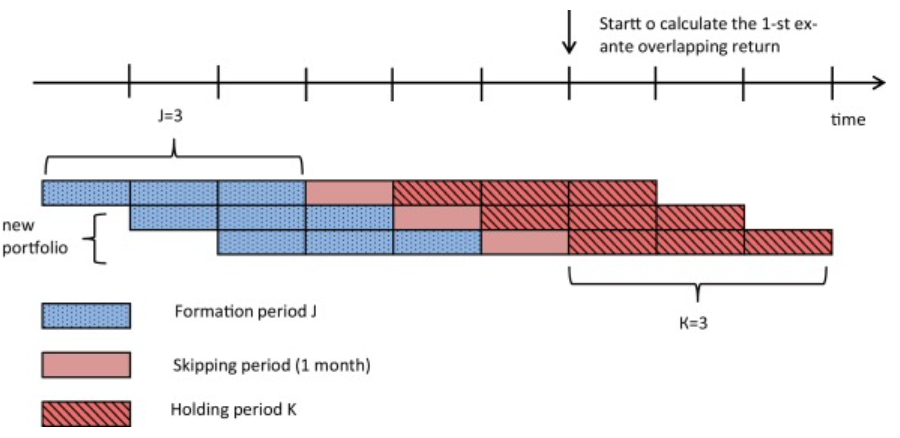
\includegraphics[width=0.7\textwidth]{momentum strategy.png}
%     \caption{Understand the momentum strategy. Source: Teplova and Mikova (2015).}
%     \label{fig:momentum strategy}
% \end{figure}

% \subsubsection{Cross-Sectional Momentum Strategy}
% A common cross-sectional momentum strategy studied in the literature involves ranking securities by their past returns and creating a zero-investment long-short portfolio consisting of:

% \begin{itemize}
% \item Long leg: Equally weighting the group of best past-performing securities (e.g., top decile), and

% \item Short leg: Equally weighting the group of worst past-performing securities (e.g., bottom decile).
% \end{itemize}

% \begin{remark}
%     There are numerous variations on this basic approach, such as those involving adjustments to weights by substituting equal weights with volatility-weighted weights. In this paper, we will discuss an example combining momentum with the Black-Litterman framework.
% \end{remark}


\subsection{Woodbury Matrix Identity}
\begin{lemma} \textbf{(Useful Lemma 1)}\label{lemma:inverse matrix sum}
Suppose $\mathbf{A}, \mathbf{B}\in \mathbb{R}^{n\times n}$, then we have
\[
(\mathbf{A}+\mathbf{B})^{-1} = \mathbf{A}^{-1}(\mathbf{\mathbf{I}}+\mathbf{B}\mathbf{A}^{-1})^{-1} = (\mathbf{\mathbf{I}}+\mathbf{A}^{-1}\mathbf{B})^{-1}\mathbf{A}^{-1}
\]
\end{lemma}
\begin{proof}
    We have
    \begin{align*}
        \mathbf{\mathbf{I}} &= (\mathbf{A}+\mathbf{B})(\mathbf{A}+\mathbf{B})^{-1}\\
        &= (\mathbf{\mathbf{I}}+\mathbf{B}\mathbf{A}^{-1})\mathbf{A}(\mathbf{A}+\mathbf{B})^{-1}\\
        \Longrightarrow (\mathbf{A}+\mathbf{B})^{-1} &=\mathbf{A}^{-1}(\mathbf{\mathbf{I}}+\mathbf{B}\mathbf{A}^{-1})^{-1}
    \end{align*}
    and 
    \begin{align*}
        \mathbf{\mathbf{I}} &= (\mathbf{A}+\mathbf{B})^{-1}(\mathbf{A}+\mathbf{B})\\
        &= (\mathbf{A}+\mathbf{B})^{-1}\mathbf{A}(\mathbf{\mathbf{I}}+\mathbf{A}^{-1}\mathbf{B})\\
        \Longrightarrow (\mathbf{A}+\mathbf{B})^{-1} &=(\mathbf{\mathbf{I}}+\mathbf{A}^{-1}\mathbf{B})^{-1}\mathbf{A}^{-1}
    \end{align*}
    Therefore, we must have
    \[
    (\mathbf{A}+\mathbf{B})^{-1} = \mathbf{A}^{-1}(\mathbf{\mathbf{I}}+\mathbf{B}\mathbf{A}^{-1})^{-1} = (\mathbf{\mathbf{I}}+\mathbf{A}^{-1}\mathbf{B})^{-1}\mathbf{A}^{-1}
    \]
\end{proof}
\begin{remark}
    Useful in the upcoming matrix computations.
\end{remark}

\begin{lemma} \textbf{(Useful Lemma 2)}\label{lemma:inverse matrix sum 2}
Suppose $\mathbf{\mathbf{I}}, \mathbf{\mathbf{P}}\in \mathbb{R}^{n\times n}$, then we have
\[
(\mathbf{\mathbf{I}}+\mathbf{\mathbf{P}})^{-1} = \mathbf{\mathbf{I}}-(\mathbf{\mathbf{I}}+\mathbf{\mathbf{P}})^{-1}\mathbf{\mathbf{P}}
\]
\end{lemma}
\begin{proof}
    We have
    \begin{align*}
        (\mathbf{\mathbf{I}}+\mathbf{\mathbf{P}})^{-1} = (\mathbf{\mathbf{I}}+\mathbf{\mathbf{P}})^{-1}(\mathbf{\mathbf{I}}+\mathbf{\mathbf{P}}-\mathbf{\mathbf{P}})=\mathbf{\mathbf{I}}-(\mathbf{\mathbf{I}}+\mathbf{\mathbf{P}})^{-1}\mathbf{\mathbf{P}}
    \end{align*}
\end{proof}
\begin{remark}
    Useful in the upcoming matrix computations.
\end{remark}

\begin{lemma} \textbf{(Useful Lemma 3)}\label{lemma:inverse matrix sum 3}
Suppose we have matrix $\mathbf{\mathbf{P}}$, $\bm{q}$, singular or non-singular, are such that $\mathbf{\mathbf{I}}+ \mathbf{\mathbf{P}}\bm{q}$ is non-singular, then we have
\[
(\mathbf{\mathbf{I}}+\mathbf{\mathbf{P}}\bm{q})^{-1}\mathbf{\mathbf{P}} = \mathbf{\mathbf{P}}(\mathbf{\mathbf{I}}+\bm{q}\mathbf{\mathbf{P}})^{-1}
\]
\end{lemma}
\begin{proof}
    Since $\mathbf{\mathbf{I}}+ \mathbf{\mathbf{P}}\bm{q}$ is non-singular and $det(\mathbf{\mathbf{I}}+ \mathbf{\mathbf{P}}\bm{q})= det(\mathbf{\mathbf{I}}+ \bm{q}\mathbf{\mathbf{P}})$,  $\mathbf{\mathbf{I}}+ \bm{q}\mathbf{\mathbf{P}}$ is also non-singular. We then have
    \begin{align*}
        \mathbf{\mathbf{P}}+ \mathbf{\mathbf{P}}\bm{q}\mathbf{\mathbf{P}}=(\mathbf{\mathbf{I}}+ \mathbf{\mathbf{P}}\bm{q})\mathbf{\mathbf{P}} &= \mathbf{\mathbf{P}}(\mathbf{\mathbf{I}}+\bm{q}\mathbf{\mathbf{P}})\\
        \Longrightarrow (\mathbf{\mathbf{I}}+\mathbf{\mathbf{P}}\bm{q})^{-1}\mathbf{\mathbf{P}} &= \mathbf{\mathbf{P}}(\mathbf{\mathbf{I}}+\bm{q}\mathbf{\mathbf{P}})^{-1}
    \end{align*}
\end{proof}
\begin{remark}
    Useful in the upcoming matrix computations.
\end{remark}


\begin{theorem} \label{theo:Binomial Inverse Theorem}\textbf{(Binomial Inverse Theorem  --- Woodbury Matrix Identity)}
    If $\mathbf{\mathbf{A}}, \mathbf{U}, \mathbf{\mathbf{B}}, \mathbf{\mathbf{V}}$ are matrices of sizes $n \times n, n \times k, k \times k, k \times n$, respectively, then
    \begin{enumerate}[label=(\alph*)]
        \item If $\mathbf{\mathbf{A}}$ and $\mathbf{\mathbf{B}}+\mathbf{\mathbf{B} \mathbf{V} \mathbf{A}}^{-1} \mathbf{U \mathbf{B}}$ are nonsingular:
        $$
        (\mathbf{\mathbf{A}}+\mathbf{U} \mathbf{B} \mathbf{\mathbf{V}})^{-1}=\mathbf{\mathbf{A}}^{-1}-\mathbf{\mathbf{A}}^{-1} \mathbf{U \mathbf{B}}\left(\mathbf{\mathbf{B}}+\mathbf{\mathbf{B} \mathbf{V} \mathbf{A}}^{-1} \mathbf{U \mathbf{B}}\right)^{-1} \mathbf{\mathbf{B} \mathbf{V} \mathbf{A}}^{-1}
        $$
        \item And (a) can be simplified to
        $$
        (\mathbf{\mathbf{A}}+\mathbf{U \mathbf{B} \mathbf{V}})^{-1}=\mathbf{\mathbf{A}}^{-1}-\mathbf{\mathbf{A}}^{-1} \mathbf{U}\left(\mathbf{\mathbf{B}}^{-1}+\mathbf{\mathbf{V} \mathbf{A}}^{-1} \mathbf{U}\right)^{-1} \mathbf{\mathbf{V} \mathbf{A}}^{-1} .
        $$
    \end{enumerate}
\end{theorem}
\begin{proof}\hfill
    \begin{enumerate}[label=(\alph*)]
        \item \begin{enumerate}[label=(\roman*)]
            \item \textbf{Method 1:} Prove by verification.

            First notice that
            $$
            (\mathbf{A}+\mathbf{U B \mathbf{V}}) \mathbf{A}^{-1} \mathbf{U B}=\mathbf{U B}+\mathbf{U B \mathbf{V} A}{ }^{-1} \mathbf{U B}=\mathbf{U}\left(\mathbf{B}+\mathbf{B \mathbf{V} A}^{-1} \mathbf{U B}\right) .
            $$
            Now multiply the matrix we wish to invert by its alleged inverse
            \begin{align*}
            & (\mathbf{A}+\mathbf{U B \mathbf{V}})\left(\mathbf{A}^{-1}-\mathbf{A}^{-1} \mathbf{U B}\left(\mathbf{B}+\mathbf{B \mathbf{V} A}^{-1} \mathbf{U B}\right)^{-1} \mathbf{B \mathbf{V} A}^{-1}\right) \\
            & =\mathbf{\mathbf{I}}_n+\mathbf{U B \mathbf{V} A}^{-1}-\mathbf{U}\left(\mathbf{B}+\mathbf{B \mathbf{V} A}^{-1} \mathbf{U B}\right)\left(\mathbf{B}+\mathbf{B \mathbf{V} A}^{-1} \mathbf{U B}\right)^{-1} \mathbf{B \mathbf{V} A}^{-1} \\
            & =\mathbf{\mathbf{I}}_n+\mathbf{U B \mathbf{V} A}^{-1}-\mathbf{U B \mathbf{V}} \mathbf{A}^{-1}\\
            &=\mathbf{\mathbf{I}}_n 
            \end{align*}
            which verifies that it is the inverse.
            \item \textbf{Method 2:} Prove by applying matrix identities.

            First, in \cref{lemma:inverse matrix sum 2}, set $\mathbf{\mathbf{P}} =\mathbf{A}^{-1}\mathbf{\mathbf{X}}$, we have \begin{align}(\mathbf{\mathbf{I}}+\mathbf{A}^{-1}\mathbf{\mathbf{X}})^{-1}= \mathbf{\mathbf{I}}-(\mathbf{\mathbf{I}}+\mathbf{A}^{-1}\mathbf{\mathbf{X}})^{-1}\mathbf{A}^{-1}\mathbf{\mathbf{X}}\label{eq:eq 1}
            \end{align}
            
            Then, by \cref{lemma:inverse matrix sum}, we have
            \begin{align*}(\mathbf{A}+\mathbf{\mathbf{X}})^{-1} &=(\mathbf{\mathbf{I}}+\mathbf{A}^{-1}\mathbf{\mathbf{X}})^{-1}\mathbf{A}^{-1} \\
            \cref{eq:eq 1}\Longrightarrow&= \left(\mathbf{\mathbf{I}}-(\mathbf{\mathbf{I}}+\mathbf{A}^{-1}\mathbf{\mathbf{X}})^{-1}\mathbf{A}^{-1}\mathbf{\mathbf{X}}\right)\mathbf{A}^{-1}\\
            &= \mathbf{A}^{-1} - (\mathbf{\mathbf{I}}+\mathbf{A}^{-1}\mathbf{\mathbf{X}})^{-1}\mathbf{A}^{-1}\mathbf{\mathbf{X}}\mathbf{A}^{-1}\\
            &= \mathbf{A}^{-1} - \mathbf{A}^{-1}(\mathbf{\mathbf{I}}+\mathbf{\mathbf{X}}\mathbf{A}^{-1})^{-1}\mathbf{\mathbf{X}}\mathbf{A}^{-1}\\
            \text{Set~} \mathbf{\mathbf{X}}=\mathbf{U}\mathbf{B}\mathbf{\mathbf{V}}\Longrightarrow&=\mathbf{A}^{-1} - \mathbf{A}^{-1}(\mathbf{\mathbf{I}}+\mathbf{U}\mathbf{B}\mathbf{\mathbf{V}}\mathbf{A}^{-1})^{-1}\mathbf{U}\mathbf{B}\mathbf{\mathbf{V}}\mathbf{A}^{-1}\\
            \text{In \cref{lemma:inverse matrix sum 3}, set~} \mathbf{\mathbf{P}}=\mathbf{U}\mathbf{B}&, \bm{q}=\mathbf{\mathbf{V}}\mathbf{A}^{-1}
            \text{, we have}\\
            \Longrightarrow
            &=\mathbf{A}^{-1} - \mathbf{A}^{-1}\mathbf{U}\mathbf{B}(\mathbf{\mathbf{I}}+\mathbf{\mathbf{V}}\mathbf{A}^{-1}\mathbf{U}\mathbf{B})^{-1}\mathbf{\mathbf{V}}\mathbf{A}^{-1}\\
            \mathbf{B}~\text{is invertible}\Longrightarrow&=\mathbf{\mathbf{A}}^{-1}-\mathbf{\mathbf{A}}^{-1} \mathbf{U \mathbf{B}}\left(\mathbf{B}^{-1}(\mathbf{\mathbf{B}}+\mathbf{\mathbf{B} \mathbf{V} \mathbf{A}}^{-1} \mathbf{U \mathbf{B}})\right)^{-1} \mathbf{ \mathbf{V} \mathbf{A}}^{-1}\\
            &=\mathbf{\mathbf{A}}^{-1}-\mathbf{\mathbf{A}}^{-1} \mathbf{U \mathbf{B}}\left(\mathbf{\mathbf{B}}+\mathbf{\mathbf{B} \mathbf{V} \mathbf{A}}^{-1} \mathbf{U \mathbf{B}}\right)^{-1} \mathbf{\mathbf{B} \mathbf{V} \mathbf{A}}^{-1}
            \end{align*}
        Therefore, we must have
        \[
        (\mathbf{\mathbf{A}}+\mathbf{U} \mathbf{B} \mathbf{\mathbf{V}})^{-1}=\mathbf{\mathbf{A}}^{-1}-\mathbf{\mathbf{A}}^{-1} \mathbf{U \mathbf{B}}\left(\mathbf{\mathbf{B}}+\mathbf{\mathbf{B} \mathbf{V} \mathbf{A}}^{-1} \mathbf{U \mathbf{B}}\right)^{-1} \mathbf{\mathbf{B} \mathbf{V} \mathbf{A}}^{-1}
        \]
        provided $\mathbf{B}$ is non-singular, and $\mathbf{\mathbf{I}}+\bm{q}\mathbf{\mathbf{P}}=\mathbf{\mathbf{I}}+\mathbf{\mathbf{V} \mathbf{A}}^{-1}\mathbf{U}\mathbf{B}$ $\mathbf{B}$ is non-singular as it's restricted by the conditions in \cref{lemma:inverse matrix sum 3}.
        \end{enumerate}
        \item Since $\mathbf{\mathbf{B}}+\mathbf{\mathbf{B} \mathbf{V} \mathbf{A}}^{-1} \mathbf{U \mathbf{B}} = \mathbf{B} (\mathbf{\mathbf{I}}+\mathbf{\mathbf{V} \mathbf{A}}^{-1} \mathbf{U \mathbf{B}})$ is nonsingular, we must have  {\color{C6}$\mathbf{\mathbf{B}}$ is invertible}. Then the two $\mathbf{\mathbf{B}}$ terms flanking the quantity inverse in the right-hand side can be replaced with $\left(\mathbf{\mathbf{B}}^{-1}\right)^{-1}$, which simplifies (a) to
        $$
        (\mathbf{\mathbf{A}}+\mathbf{U \mathbf{B} \mathbf{V}})^{-1}=\mathbf{\mathbf{A}}^{-1}-\mathbf{\mathbf{A}}^{-1} \mathbf{U}\left(\mathbf{\mathbf{B}}^{-1}+\mathbf{\mathbf{V} \mathbf{A}}^{-1} \mathbf{U}\right)^{-1} \mathbf{\mathbf{V} \mathbf{A}}^{-1} .
        $$
    \end{enumerate}
\end{proof}

\begin{remark}
    This matrix identity is important in proving some properties in relation to the Black-Litterman model.
\end{remark}

\begin{corollary}\label{coro:black-Litterman Matrix Result} \textbf{(A Useful Result for Black-Litterman Model Construction)}
Suppose $0<\tau<1$, $\tau \in \mathbb{R}$, $\mathbf{\Sigma}\in \mathbb{R}^{n\times n}$, $\mathbf{P}\in \mathbb{R}^{k\times n}$, and $\mathbf{\Omega} \in \mathbb{R}^{k\times k}$. Then, we have
\[
\left[(\tau \mathbf{\Sigma})^{-1}+\mathbf{P}^\top \mathbf{\Omega}^{-1} \mathbf{P}\right]^{-1} = \tau \mathbf{\Sigma}-\tau \mathbf{\Sigma} \mathbf{P}^\top (\mathbf{\Omega}+\mathbf{P}\tau \mathbf{\Sigma} \mathbf{P}^\top)^{-1} \mathbf{P} \tau \mathbf{\Sigma}
\]
\end{corollary}
\begin{proof}
    In \cref{theo:Binomial Inverse Theorem}, set $\mathbf{A}=(\tau \mathbf{\Sigma})^{-1}$, $\mathbf{U}=\mathbf{P}^\top$, $\mathbf{B}=\mathbf{\Omega}^{-1}$, $\mathbf{\mathbf{V}}=\mathbf{P}$, then we have
    \begin{align*}
        &\quad \left[(\tau \mathbf{\Sigma})^{-1}+\mathbf{P}^\top \mathbf{\Omega}^{-1} \mathbf{P}\right]^{-1}\\
        &= \left((\tau \mathbf{\Sigma})^{-1}\right)^{-1}- \left((\tau \mathbf{\Sigma})^{-1}\right)^{-1}\mathbf{P}^\top \left(\left(\mathbf{\Omega}^{-1}\right)^{-1}+\mathbf{P}\left((\tau \mathbf{\Sigma})^{-1}\right)^{-1}\mathbf{P}^\top\right)^{-1}\mathbf{P}\left((\tau \mathbf{\Sigma})^{-1}\right)^{-1}\\
        &=\tau \mathbf{\Sigma}-\tau \mathbf{\Sigma} \mathbf{P}^\top \left(\mathbf{\Omega}+\mathbf{P}\tau \mathbf{\Sigma} \mathbf{P}^\top\right)^{-1}\mathbf{P}\tau \mathbf{\Sigma}\\
    \end{align*}
    Hence, we obtain
    \[
    \left[(\tau \mathbf{\Sigma})^{-1}+\mathbf{P}^\top \mathbf{\Omega}^{-1} \mathbf{P}\right]^{-1} = \tau \mathbf{\Sigma}-\tau \mathbf{\Sigma} \mathbf{P}^\top (\mathbf{\Omega}+\mathbf{P}\tau \mathbf{\Sigma} \mathbf{P}^\top)^{-1} \mathbf{P} \tau \mathbf{\Sigma}
    \]
\end{proof}

\subsection{Generalized Least Squares}
\begin{enumerate}
    \item \textbf{Data:} 
    
    In standard linear regression models we observe data $\left\{y_i, x_{i j}\right\}_{i=1, \ldots, n, j=2, \ldots, k}$ on $n$ statistical units. The response values are placed in a vector $\bm{y}=\left(y_1, \ldots, y_n\right)^{\top}$, and the predictor values are placed in the design matrix $\mathbf{X}=\left(\mathbf{x}_1^{\top}, \ldots, \mathbf{x}_n^{\top}\right)$, where $\mathbf{x}_i=\left(1, x_{i 2}, \ldots, x_{i k}\right)$ is a vector of the $k$ predictor variables / features (including a constant) for the $i^{th}$ unit. 
    \item \textbf{Model:} 
    
    The model forces the conditional mean of $\bm{y}$ given $\mathbf{X}$ to be a linear function of $\mathbf{X}$, i.e.$
\mathbb{E}[\bm{y}|\mathbf{X}] = \mathbf{X}\bm{\bm{\beta}}
$, and assumes the conditional variance of the error term $\bm{\varepsilon}\in \mathbb{R}^{n}$ given $\mathbf{X}$ is a known non-singular covariance matrix $\mathbf{\Omega}\in \mathbb{R}^{n\times n}$. This is usually written as
$$
\bm{y}=\mathbf{X} \bm{\bm{\beta}}+\bm{\bm{\varepsilon}}, \quad \EE[\bm{\bm{\varepsilon}} | \mathbf{X}]=0, \operatorname{Cov}[\bm{\bm{\varepsilon}} | \mathbf{X}]=\mathbf{\Omega} .
$$
Here $\bm{\bm{\beta}} \in \mathbb{R}^{k}$ is a vector of unknown constants (known as "regression coefficients") that must be estimated from the data.
\item \textbf{Loss Function:} 

Suppose $\mathbf{b}$ is a candidate estimate for $\bm{\beta}$. Then the residual vector for $\mathbf{b}$ will be $\bm{y}-\mathbf{X b}$. The generalized least squares method estimates $\bm{\beta}$ by minimizing the squared Mahalanobis length of this residual vector:
$$
\begin{aligned}
\hat{\bm{\beta}} & =\underset{b}{\operatorname{argmin}}\quad (\bm{y}-\mathbf{X} \mathbf{b})^{\top} \mathbf{\Omega}^{-1}(\bm{y}-\mathbf{X} \mathbf{b}) \\
& =\underset{b}{\operatorname{argmin}} \quad \bm{y}^{\top} \mathbf{\Omega}^{-1} \bm{y}+(\mathbf{X} \mathbf{b})^{\top} \mathbf{\Omega}^{-1} \mathbf{X} \mathbf{b}-\bm{y}^{\top} \mathbf{\Omega}^{-1} \mathbf{X} \mathbf{b}-(\mathbf{X} \mathbf{b})^{\top} \mathbf{\Omega}^{-1} \bm{y},
\end{aligned}
$$
where the last two terms evaluate to scalars, resulting in
$$
\hat{\bm{\beta}}=\underset{b}{\operatorname{argmin}} \quad \bm{y}^{\top} \mathbf{\Omega}^{-1} \bm{y}+\mathbf{b}^{\top} \mathbf{X}^{\top} \mathbf{\Omega}^{-1} \mathbf{X} \mathbf{b}-2 \mathbf{b}^{\top} \mathbf{X}^{\top} \mathbf{\Omega}^{-1} \bm{y}
$$
\item \textbf{Solve for the GLS Estimator:}

This objective is a quadratic form in $\mathbf{b}$.
Taking the gradient of this quadratic form with respect to $\mathbf{b}$ and equating it to zero (when $\mathbf{b}=\hat{\bm{\beta}}$ ) gives
$$
2 \mathbf{X}^{\top} \mathbf{\Omega}^{-1} \mathbf{X} \hat{\bm{\beta}}-2 \mathbf{X}^{\top} \mathbf{\Omega}^{-1} \bm{y}=0
$$
Therefore, the minimum of the objective function can be computed yielding the explicit formula:
$$
\hat{\bm{\beta}}_{GLS}=\left(\mathbf{X}^{\top} \mathbf{\Omega}^{-1} \mathbf{X}\right)^{-1} \mathbf{X}^{\top} \mathbf{\Omega}^{-1} \bm{y}
$$
The quantity $\mathbf{\Omega}^{-1}$ is known as the precision matrix (or dispersion matrix), a generalization of the diagonal weight matrix.
\end{enumerate}


\subsubsection{Properties of GLS Estimator}
The GLS estimator is 
\begin{itemize}
    \item unbiased,
    \item consistent,
    \item efficient,
    \item asymptotically normal
    \item $\EE[\hat{\bm{\beta}} | \mathbf{X}]=\bm{\beta}$ and $\operatorname{Cov}[\hat{\bm{\beta}} | \mathbf{X}]=\left(\mathbf{X}^{\top} \Omega^{-1} \mathbf{X}\right)^{-1}$.
\end{itemize}    

\begin{property}
    \textbf{(Understanding GLS)} GLS is equivalent to applying ordinary least squares to a linearly transformed version of the data.
\end{property} 
\begin{solution}
    To see this, factor $\mathbf{\Omega}=\mathbf{C C}^{\top}$ using the Cholesky decomposition. Then if we pre-multiply both sides of the equation $\bm{y}=\mathbf{X} \bm{\beta}+\bm{\varepsilon}$ by $\mathbf{C}^{-1}$, i.e.
    \[
    \bm{y}=\mathbf{X} \bm{\beta}+\bm{\varepsilon} \quad \Longrightarrow \quad \mathbf{C}^{-1}\bm{y}=\mathbf{C}^{-1}\mathbf{X} \bm{\beta}+\mathbf{C}^{-1}\bm{\varepsilon}
    \]
    we get an equivalent linear model \[\bm{y}^*=\mathbf{X}^* \bm{\beta}+\bm{\varepsilon}^*\]
    where $\bm{y}^*=\mathbf{C}^{-1} \bm{y}, \mathbf{X}^*=\mathbf{C}^{-1} \mathbf{X}$, and $\bm{\varepsilon}^*=\mathbf{C}^{-1} \bm{\varepsilon}$. 
    
    In this model \begin{align*}Cov=\mathbb{V}\left[\bm{\varepsilon}^* | \mathbf{X}\right]&=\mathbb{E}\left[(\bm{\varepsilon}^*-\mathbb{E}[\bm{\varepsilon}^*])(\bm{\varepsilon}^*-\mathbb{E}[\bm{\varepsilon}^*])^\top | \mathbf{X}\right]\\
    &=\mathbb{E}\left[C^{-1}(\bm{\varepsilon}-\mathbb{E}[\bm{\varepsilon}])(\bm{\varepsilon}-\mathbb{E}[\bm{\varepsilon}])^\top (C^{-1})^\top| \mathbf{X}\right]\\
    &=\mathbf{C}^{-1} \mathbb{V}[\bm{\varepsilon}| \mathbf{X}]\left(\mathbf{C}^{-1}\right)^{\top}\\
    &=\mathbf{C}^{-1} \mathbf{\Omega}\left(\mathbf{C}^{-1}\right)^{\top}\\
    &=\mathbf{I}
    \end{align*}
    where $\mathbf{I}$ is the identity matrix. 
    
    Thus we can efficiently estimate $\bm{\beta}$ by applying Ordinary least squares (OLS) to the transformed data, which requires minimizing
$$
\left(\bm{y}^*-\mathbf{X}^* \bm{\beta}\right)^{\top}\left(\bm{y}^*-\mathbf{X}^* \bm{\beta}\right)=(\bm{y}-\mathbf{X b})^{\top} \mathbf{\Omega}^{-1}(\bm{y}-\mathbf{X} \mathbf{b})
$$
This has the effect of standardizing the scale of the errors and "de-correlating" them. Since OLS is applied to data with homoscedastic errors, the GaussMarkov theorem applies, and therefore the GLS estimate is the best linear unbiased estimator for $\bm{\beta}$.
\end{solution}

\subsection{Bayesian Statistical Model} \label{sec:Bayesian Statistical Model}
A Bayesian statistical model consists of:
\begin{enumerate}
\item An unknown target parameter $\bm{\theta}\in\Theta \subseteq \mathbb{R}^{\ell}$.  
    \item A vector-valued random variable $\bm{x} \in \mathcal{X} \subseteq \mathbb{R}^d$  where realizations of $\bm{x}$ have been observed and known.
    \item $\bm{x}$ is assumed to be distributed according to the likelihood function $f(\bm{x} | \bm{\theta})$. After conditioning on $\bm{\theta}$, $f(\bm{x} | \bm{\theta})$ forms a density on the data space $\mathcal{X} \subseteq \mathbb{R}^d$. 
    \item A prior density $\pi(\bm{\theta})$ of $\bm{\theta}$ on $\Theta$.
    \item The posterior  is the density $p(\bm{\theta}|\bm{x})$ on $\Theta$ proportional to $f(\bm{x} | \bm{\theta}) \pi(\bm{\theta})$, i.e.
    \[
    p(\bm{\theta}|\bm{x}) = C f(\bm{x} | \bm{\theta}) \pi(\bm{\theta})
    \]
    and the normalization factor $C$ can be calculated using the fact that $\int p(\bm{\theta}|\bm{x}) = 1$.
\end{enumerate}

{\color{C6}\textbf{Intuition:}} The Bayesian framework can be viewed as a journey of finding the right distribution for $\bm{\theta}$. Initially, you have a rough idea of what the distribution of $\bm{\theta}$ might be, which is called the prior, $\pi(\bm{\theta})$. Next, you use the ``real" observations of $\bm{x}$ to update your understanding of the latent parameter $\bm{\theta}$'s distribution, denoted by $p(\bm{\theta}|\bm{x})$. In the case of $\ell=d=1$, we have
\[
p\left(\theta | X_1=x_1, \ldots, X_n=x_n\right) \propto f\left(X_1=x_1, \ldots, X_n=x_n |\theta\right) \pi(\theta)
\]
As more and more observations are provided, you will eventually find the true distribution of $\bm{\theta}$, or a distribution around the true value of $\bm{\theta}$ with a narrow interval.
\begin{remark}\hfill
\begin{enumerate}
    \item  In Bayesian statistics, all statistical inference is based on the posterior $p(\bm{\theta}|\bm{x})$.
    \item In the Bayesian context, $p$ is used more specifically to denote these probability distributions related to Bayesian inference, whereas the letter $f$ is more general and can represent any probability density or mass function, whether in a Bayesian or frequentist context.
    \item When using the likelihood function, we can drop its coefficient, which essentially means that only the relative value of $f(\bm{x} | \bm{\theta})$ matters.

For instance, if $\bm{x} | \bm{\theta} \sim \mathcal{N}(0,1)$, then $f(\bm{x} | \bm{\theta}) = \frac{1}{\sqrt{2 \pi}} e^{-x^2 / 2}$. We could use $f'(\bm{x} | \bm{\theta}) = e^{-x^2 / 2}$ instead, because the scale, i.e., $c = \frac{1}{\sqrt{2 \pi}}$, is not important.

This occurs because when maximizing the likelihood function to solve for the MLE estimator, both $c \cdot f(\bm{x} | \bm{\theta})$ and $f'(\bm{x} | \bm{\theta})$ will have the same maximum. Additionally, when calculating the normalization factor $C$ in Bayesian statistics, both $c \cdot f(\bm{x} | \bm{\theta})$ and $f'(\bm{x} | \bm{\theta})$ will produce the same posterior due to the way we compute the posterior. As a result, we do not concern ourselves with the scale.
\end{enumerate}
\end{remark}


\begin{theorem}\label{theo:A Useful Theorem}
    \textbf{(A Useful Theorem)} If a multivariate normal random variable $\boldsymbol{\theta}\in \mathbb{R}^{k}$ has density $p(\boldsymbol{\theta})$ and 
    \[
    -2 \log p(\boldsymbol{\theta})=\boldsymbol{\theta}^{\top} \mathbf{M} \boldsymbol{\theta}-2 \boldsymbol{u}^{\top} \boldsymbol{\theta}+(\text{ terms without }\boldsymbol{\theta})
    \] 
    where $\mathbf{M}\in \mathbb{R}^{k\times k}$ is symmetric and invertible, then 
    \[
    \mathbb{V}[\boldsymbol{\theta}]=\mathbf{M}^{-1} \text{ and ~} \mathbb{E} [\boldsymbol{\theta}]=\mathbf{M}^{-1} \boldsymbol{u}.
    \]

\end{theorem}
\begin{solution}
    For $\mathbf{M}$ symmetric and invertible, we have
    \begin{align*}
    -2 \log p(\boldsymbol{\theta})&=\boldsymbol{\theta}^{\top} \mathbf{M} \boldsymbol{\theta}-2 \boldsymbol{u}^{\top} \boldsymbol{\theta}+(\text{ terms without }\boldsymbol{\theta})\\
    &=\boldsymbol{\theta}^{\top} \mathbf{M} \boldsymbol{\theta}-2 \boldsymbol{u}^{\top}\mathbf{M}^{-1}\mathbf{M} \boldsymbol{\theta}+(\text{ terms without }\boldsymbol{\theta})\\
    &=(\boldsymbol{\theta}-\mathbf{M}^{-1}\boldsymbol{u})^{\top} \mathbf{M}(\boldsymbol{\theta}-\mathbf{M}^{-1}\boldsymbol{u})-\bm{u}^{\top} \mathbf{M}^{-1} \boldsymbol{u}+(\text{ terms without }\boldsymbol{\theta})\\
    &=(\boldsymbol{\theta}-\mathbf{M}^{-1}\boldsymbol{u})^{\top} \mathbf{M}(\boldsymbol{\theta}-\mathbf{M}^{-1}\boldsymbol{u})+(\text{ terms without }\boldsymbol{\theta})
    \end{align*}
    Since $p(\boldsymbol{\theta})$ is a density function, we msut have
    \begin{align*}
    1=\int p(\boldsymbol{\theta}) d\bm{\theta} &= \int \exp\left[-\frac{1}{2}\left((\boldsymbol{\theta}-\mathbf{M}^{-1}\boldsymbol{u})^{\top} \mathbf{M}(\boldsymbol{\theta}-\mathbf{M}^{-1}\boldsymbol{u})+(\text{ terms without }\boldsymbol{\theta})\right)\right] d\bm{\theta}\\
    &=\sqrt{(2 \pi)^k|\mathbf{M}^{-1}|}\cdot \exp\left[-\frac{1}{2}\left((\text{ terms without }\boldsymbol{\theta})\right)\right]
    \end{align*}
    \[
    \Longrightarrow \frac{1}{\sqrt{(2 \pi)^k|\mathbf{M}^{-1}|}} = \exp\left[-\frac{1}{2}\left((\text{ terms without }\boldsymbol{\theta})\right)\right]
    \]
    Hence, we get
    \begin{align*}
    p(\boldsymbol{\theta}) &= \exp\left[-\frac{1}{2}\left((\boldsymbol{\theta}-\mathbf{M}^{-1}\boldsymbol{u})^{\top} \mathbf{M}(\boldsymbol{\theta}-\mathbf{M}^{-1}\boldsymbol{u})+(\text{ terms without }\boldsymbol{\theta})\right)\right]\\
    &= \frac{1}{\sqrt{(2 \pi)^k|\mathbf{M}^{-1}|}} \exp\left[-\frac{1}{2}\left((\boldsymbol{\theta}-\mathbf{M}^{-1}\boldsymbol{u})^{\top} \mathbf{M}(\boldsymbol{\theta}-\mathbf{M}^{-1}\boldsymbol{u})\right)\right]
    \end{align*}
    This is the density function for a multi-variable Gaussian distribution $\mathcal{N}\left(\mathbf{M}^{-1}\boldsymbol{u}, \mathbf{M}^{-1}\right)$; therefore, we can view parameter $\bm{\theta}$ as 
    \[
    \bm{\theta} \sim \mathcal{N}\left(\mathbf{M}^{-1}\boldsymbol{u}, \mathbf{M}^{-1}\right)
    \]
    Then, we must have
    \[
    \mathbb{V}[\boldsymbol{\theta}]=\mathbf{M}^{-1} \text{ and ~} \mathbb{E} [\boldsymbol{\theta}]=\mathbf{M}^{-1} \boldsymbol{u}.
    \]
\end{solution}
% \subsubsection{Conjugate Prior}

\subsection{Multivariate log-normal}\label{subsec:log-normal}
If $\boldsymbol{X} \sim \mathcal{N}(\boldsymbol{\mu}, \boldsymbol{\Sigma})$ is a multivariate normal distribution, then $Y_i=\exp \left(X_i\right)$ has a multivariate log-normal distribution.  The exponential is applied elementwise to the random vector $\boldsymbol{X}$. The mean of $\boldsymbol{Y}$ is
$$
\mathrm{E}[\boldsymbol{Y}]_i=e^{\mu_i+\frac{1}{2} \Sigma_{i i}}
$$
and its covariance matrix is
$$
\operatorname{Var}[\boldsymbol{Y}]_{i j}=e^{\mu_i+\mu_j+\frac{1}{2}\left(\Sigma_{i i}+\Sigma_{j j}\right)}\left(e^{\Sigma_{i j}}-1\right)
$$


%%%%%%%%%%%%%%%%%%%%%%%%%%%%%%%%%%%%%%%%%%%%%
\newpage
\section{Fictional Market Sample}\label{sec:Fictional Market Sample}
{\color{C6} \textbf{Motivation:} We introduce the example used in the paper (He and Litterman (2002)) regarding the international equity market so as to better  illustrate our point.}

Data has been provided for the index volatility, equilibrium portfolio weight, and implied returns. The weighting is based on the market capitalization of each market and the expected returns are implied by the market prices. 

\begin{table}[!htp]
\centering
    \caption{Market Data}
    \label{tab:market data}
\begin{tabular}{|l|l|l|l|}
\hline Country & $\begin{array}{l}\text { Equity Index}\\ \text{ Volatility }
(\%)\end{array}$ & $\begin{array}{l}\text { Equilibrium}\\ \text{ Portfolio Weight }(\%)\end{array}$ & $\begin{array}{l}\text { Equilibrium} \\
\text { Expected  Returns }(\%)\end{array}$ \\
\hline Australia & 16.0 & -1.097079 & 3.9 \\
\hline Canada & 20.3 & 18.74685 & 6.9 \\
\hline France & 24.8 & 4.287915 & 8.4 \\
\hline Germany & 27.1 & 2.364488 & 9.0 \\
\hline Japan & 21.0 & 11.429539 & 4.3 \\
\hline UK & 20.0 & 13.61645 & 6.8 \\
\hline USA & 18.7 & 52.082372 & 7.6 \\
\hline
\end{tabular}
\end{table}
Additionally, we provide the covariance matrix for this dataset.
\begin{table}[!htp]
\centering
    \caption{Covariance Matrix of Returns}
    \label{tab:covariance matrix}
\begin{tabular}{|l|l|l|l|l|l|l|l|}
\hline & AUS & CAN & FRA & GER & JAP & UK & USA \\
\hline AUS & 0.0256 & 0.01585 & 0.018967 & 0.02233 & 0.01475 & 0.016384 & 0.014691 \\
\hline CAN & 0.01585 & 0.041209 & 0.033428 & 0.036034 & 0.027923 & 0.024685 & 0.024751 \\
\hline FRA & 0.018967 & 0.033428 & 0.061504 & 0.057866 & 0.018488 & 0.038837 & 0.030979 \\
\hline GER & 0.02233 & 0.036034 & 0.057866 & 0.073441 & 0.020146 & 0.042113 & 0.033092 \\
\hline JAP & 0.01475 & 0.013215 & 0.018488 & 0.020146 & 0.0441 & 0.01701 & 0.012017 \\
\hline UK & 0.016384 & 0.024685 & 0.038837 & 0.042113 & 0.01701 & 0.04 & 0.024385 \\
\hline USA & 0.014691 & 0.029572 & 0.030979 & 0.033092 & 0.012017 & 0.024385 & 0.034969 \\
\hline
\end{tabular}
\end{table}
Lastly, we set the risk-free rate to be $2\%$; that is,
\begin{align}
    r_f=2\% \label{eq:risk free rate}
\end{align}

\newpage
\section{Mean-Variance Optimization}
The MVO is a single period model. We will use the fictional data in \cref{sec:Fictional Market Sample} to better illustrate our points along the way.

\subsection{Financial Concepts}\label{sec:financial concepts}
\begin{definition}\textbf{(Rate of Return)} We define the \textbf{rate of return (RoR or $r$)} as 
\[
r=\text{rate of return} = \frac{\text{amount received}-\text{amount invested}}{\text{amount invested}}
\]
\end{definition}
\begin{definition}\textbf{(Total Return)} We define the \textbf{total return (total R or $R$)} as 
\[
R=\text{total return} = \frac{\text{amount received}}{\text{amount invested}}
\]
\end{definition}
\begin{remark}\hfill
\begin{enumerate}[label=(\alph*)]
    \item In some context, the ``total return'' defined above is called ``gross return'' and ``rate of return'' is called ``total return''.
\end{enumerate}
    Such definition is \textbf{consistent} for both vanilla trade and short sale. To be specific, we have
    \begin{enumerate}
        \item Suppose we are in a vanilla trade, where you invest $X_0$ dollars and get $X_1$ dollars from this investment ($X_0>0$). Then your RoR is $r=\frac{X_1-X_0}{X_0}$, and total return is $R=\frac{X_1}{X_0}$. That is,
\[
\text{vanilla trade}: \begin{cases}
\text{pay} \quad X_0 \\
\text{get} \quad X_1
\end{cases}
\Longrightarrow
\begin{cases}
\text{RoR}=r= \frac{X_1-X_0}{X_0}\\
R=\frac{X_1}{X_0}
\end{cases}
\]
\item Suppose we are shorting, where you invest $-X_0$ dollars and get $-X_1$ dollars from this investment  ($X_0>0$). Then your RoR is $r=\frac{-X_1-(-X_0)}{-X_0}$, and total return is $R=\frac{-X_1}{-X_0}$. That is,
\[
\text{short sale}: \begin{cases}
\text{pay} \quad -X_0 \\
\text{get} \quad -X_1
\end{cases}
\Longrightarrow
\begin{cases}
\text{RoR}=r= \frac{X_1-X_0}{X_0}\\
R=\frac{X_1}{X_0}
\end{cases}
\]
    \end{enumerate}
\end{remark}

\begin{definition}
    \textbf{(Relative Weighted Portfolio)} Suppose we invested in $n$ asset where the amount invested in the $i$-th asset is $X_{0i}$, $i=1,2,\ldots, n$, and the total capital invested is $X_0$. Then, we have
    \[
    X_0=\sum_{i=1}^n X_{0i}.
    \]
    Then, the equation above describes an allocation/portfolio.
    
    It's usually better to rewrite the above equation as
    \[
    X_0=\sum_{i=1}^n w_iX_{0}.
    \]
    where $w_i =\frac{X_{0i}}{X_{0}}$, and $\sum_{i=1}^n w_i = 1$.
    We call such formulation \textbf{relative weighted portfolio}. If we allow shorting, $X_{0i}$ can be negative, and so does the corresponding $w_i$.
\end{definition}
\begin{remark}
    The reason for us to formulate the portfolio as the one with relative weights are 
    \begin{enumerate}
        \item More Intuitive: It is easier to interpret a statement such as "thirty percent of one’s budget is invested in xyz" than "his investment consists, among others, of a thousand shares of xyz".
        \item Reduce computational complexity: Results in simpler forms for the computation in the following different allocation
        frameworks.
    \end{enumerate} 
\end{remark}

\begin{definition} \textbf{(The Total Return of The Portfolio)}
    The total return of the portfolio is
$$
R_{p}:=\frac{\text { amount received }}{\text { amount invested }}=\frac{\sum_{i=1}^{n} R_{i} w_{i} X_{0}}{X_{0}}=\sum_{i=1}^{n} R_{i} w_{i} .
$$
\end{definition}

Suppose we want to invest in $n$ different assets $A_1, A_2,\ldots, A_n$ and the rate of return for each of them in one period can be viewed as a random variable $r_i, i=1,2,\ldots, n$. Put this in the vector format, we can rewrite it as $\bm{r}=(r_1, r_2, \ldots, r_n)\in \mathbb{R}^n$.
\begin{definition}\textbf{( The Portfolio Rate of Return)}\label{def:portfolio rate of return}
    Then, the portfolio rate of return is
$$
r_p = \frac{\text{amount received}-\text{amount invested}}{\text{amount invested}} =\frac{X_{0}\left(\sum_{i=1}^{n} R_{i} w_{i}-\sum_{i=1}^{n} w_{i}\right)}{X_{0}} =\sum_{i=1}^{n} r_{i} w_{i} = \bm{w}^{\top} \bm{r}
$$
where $w:=\left(w_{1}, \ldots, w_{n}\right)$.
\end{definition}

\begin{definition}\label{def:Expected Return of the Assets}
    \textbf{(Expected Return of the Assets)} Since each $r_i$ can be viewed as a random variable, we can then define the expected return of assets as
\[
\bm{\mu}:= \mathbb{E}[\bm{r}]\in \mathbb{R}^n
\]
where $\bm{r}=(r_1, r_2, \ldots, r_n)\in \mathbb{R}^n$.
\end{definition}

\begin{definition}\label{def:(Expected Return of the Portfolio} \textbf{(Expected Return of the Portfolio)}
    Then, the expected return of the portfolio is  
$$
\mu_p:=\mathbb{E}\left[r_{p}\right] =\mathbb{E}\left[\bm{w}^{\top} \bm{r}\right]
=\bm{w}^{\top} \mathbb{E}[\bm{r}] 
=\bm{w}^{\top} \bm{\mu}.
$$
where $\bm{\mu}:=\mathbb{E}[\bm{r}]$. 
\end{definition}
\begin{remark}\hfill
\begin{enumerate}
    \item Sometimes, we use the notation $\bm{\mu}:=\mathbb{E}\left[\bm{r}\right]$.
    \item Since all the $r_i$'s are random variables, $\mu_p$ is a random variable.
\end{enumerate}
    
\end{remark}

\begin{definition}\label{def:The Variance of the Portfolio Return}
    \textbf{(The Variance of the Portfolio Rate of Return)} The variance of the portfolio return is given by
$$
\begin{aligned}
\sigma_p^2 =\VV\left[r_{p}\right] & =\mathbb{E}\left[\left(r_{p}-\mathbb{E}\left[r_{p}\right]\right)^{2}\right] \\
& =\mathbb{E}\left[\left(\bm{w}^{\top} \bm{r}-\bm{w}^{\top} \mathbb{E}[\bm{r}]\right)^{2}\right] \\
& =\mathbb{E}\left[\bm{w}^{\top}(\bm{r}-\mathbb{E}[\bm{r}])(\bm{r}-\mathbb{E}[\bm{r}])^{\top} \bm{w}\right] \\
& =\bm{w}^{\top} \mathbb{E}\left[(\bm{r}-\mathbb{E}[\bm{r}])(\bm{r}-\mathbb{E}[\bm{r}])^{\top}\right] \bm{w} \\
& =\bm{w}^{\top} \operatorname{var}[\bm{r}] \bm{w} \\
& =\bm{w}^{\top} \mathbf{\Sigma} \bm{w},
\end{aligned}
$$
where $\mathbf{\Sigma}:=\operatorname{var}[\bm{r}]$ is the covariance matrix of returns. $\mathbf{\Sigma}$ is symmetric and semi-positive definite.
\end{definition}

\begin{definition} \label{def: Risk Preference}
    \textbf{(Risk Preference)}
    \begin{enumerate}
        \item Risk Averse: Risk is bad and should be minimized.
        \item Risk-preferring: Risk is good, like taking risks.
        \item Risk Neutral: Don't like or hate risk.
    \end{enumerate}
\end{definition}

\begin{definition} \label{def: Non-satiation}
    \textbf{(Non-satiation)}
    An investor is Non-satiation means if everything else holds fixed, the investor always wants more money/higher return.
\end{definition}

\begin{definition}\textbf{(zero-cost portfolio of risky securities)}
    A zero-cost portfolio of risky securities is a portfolio $\bm{w}$ such that
$$
\bm{w}^{\top} \bm{e}=0
$$
where $\bm{e}=(1,1,\ldots, 1)\in \mathbb{R}^n$.
\end{definition}

\begin{definition}\textbf{(market neutral portfolio of risky securities)}
    A market neutral portfolio of risky securities is a portfolio $\bm{w}$ such that
$$
\bm{w}^{\top} \bm{\bm{\beta}}=0
$$
where $ \bm{\bm{\beta}}:=\left(\beta_{1}, \ldots, \beta_{m}\right)$ is the vector of security betas with respect to the market.
\end{definition}

\begin{definition}\label{def:Market Portfolio}\textbf{(Market Portfolio)} The market portfolio is a portfolio such that 
    \begin{enumerate}[label=(\alph*)]
  \item It consists of all securities available to investors, and
  \item each security in the market portfolio is held in proportion to its market value (market capitalization) relative to the total market value of all securities.
  \end{enumerate}
\end{definition}

%%%%%%%%%%%%%%%%%%%%%%%%%%%%%%%%%%%
\subsection{MVO With Only Risky Securities}
\subsubsection{Formulation}
{\color{C6}\textbf{Motivation:} We want to analyze the distribution of the portfolio mean rate of return.}

In the classical Mean-Variance Analysis, we need to make two basic assumptions:
\begin{assumption}\textbf{(Core Assumption)}
\begin{enumerate}
    \item The investor exhibits risk aversion  (\cref{def: Risk Preference} and non-satiation (\cref{def: Non-satiation}) preferences.
    \item The investor's initial capital is not null.
\end{enumerate}
\end{assumption}

Using the concepts and notation in \cref{sec:financial concepts}, suppose we want to invest in $n$ different assets $A_1, A_2,\ldots, A_n$ and the rate of return for each of them in one period can be viewed as a random variable $r_i, i=1,2,\ldots, n$. Put this in the vector format, we can rewrite it as $\bm{r}=(r_1, r_2, \ldots, r_n)\in \mathbb{R}^n$. From \cref{def:portfolio rate of return}, we can write the portfolio rate of return as 
\[
r_p=\bm{w}^{\top} \bm{r}
\]
where $\bm{w}:=\left(w_{1}, \ldots, w_{n}\right)\in\mathbb{R}^n$ is the vector of portfolio weights. Then, by \cref{def:Expected Return of the Assets} and \cref{def:(Expected Return of the Portfolio}, we obtain the expected return as
$$
\mu_p =\bm{w}^{\top} \bm{\mu},
$$
where $\bm{\mu}:=\mathbb{E}[\bm{r}]\in\mathbb{R}^n$ is the expected return of assets. Then, by \cref{def:The Variance of the Portfolio Return}, we get the variance of the portfolio return is given by 
\[
\sigma_p^2 =\bm{w}^{\top} \mathbf{\Sigma} \bm{w}
\]
Then, we can start to construct our MVO framework.

{\color{C6} MVO Framework:} The MVO suggests that investors should allocate their wealth by solving the one-period mean-variance optimization (MVO) problem 
\begin{align*}
    \min _{\bm{w}} \quad & \frac{1}{2} \bm{w}^{\top} \mathbf{\Sigma} \bm{w} \\
    \text {s.t.} \quad  & \bm{w}^{\top} \bm{\mu}=\mu_{p}, \quad  
 \bm{w}^{\top} \bm{e}=1
\end{align*}
where
\begin{itemize}
    \item $\bm{e}:=(1, \ldots, 1) \in \mathbb{R}^{n}$,
    \item $\bm{w} \in \mathbb{R}^{n}$ is the vector of portfolio weights,
    \item $\bm{\mu} \in \mathbb{R}^{n}$ is the vector of expected returns,
    \item $\mathbf{\Sigma} \in \mathbb{R}^{n \times n}$ is the covariance matrix of returns, and
    \item $\mu_{p} \geq 0$ is the desired level of portfolio return.
\end{itemize}
\begin{remark}\hfill
\begin{enumerate}
\item Term $\bm{\mu}$ and $\mathbf{\Sigma}$ shall be treated as known and should be provided by the investor.
    \item This is often called the Variance-Minimization formulation (or Risk-Minimization formulation). In such formulation, we treat variable $\mu_p$ as a fixed value. And for every fixed $\mu_p$, there is a $\bm{w}_p$ that minimizes $\bm{w}^\top\mathbf{\Sigma}\bm{w}$ which gives the minimized variance of portfolio return $\sigma_p=\sqrt{\bm{w}_p^\top\mathbf{\Sigma}\bm{w}_p}$.
    \item We assume that $\mu_{p}>0$ is chosen such that a solution to the MVO exists. In general the first constraint is frequently changed to $\bm{w}^{\top} \bm{\mu} \leq \mu_{p}$.\label{re:general MVO}
    \item There are in several different but mathematically equivalent formulations of the MVO problem. For example:

    \textbf{(The Expected Return Maximization Formulation)} The expected return maximization formulation is stated as
\begin{align*}
\max _{\bm{w}} & \quad \bm{w}^{\top} \bm{\mu} \\
\text {s.t.} \quad & \bm{w}^{\top} \mathbf{\Sigma} \bm{w}=\sigma_{p}^{2}, \quad  \bm{w}^{\top} \bm{e}=1
\end{align*}
where $\sigma_{p}^{2}$ is the desired level of portfolio variance (risk) viewed as fixed variable.

    \textbf{(The Risk Aversion Formulation)} The risk aversion formulation is stated as
\begin{align*}
&\max _{\bm{w}}\quad  \bm{w}^{\top} \bm{\mu}-\frac{\lambda}{2} \bm{w}^{\top} \mathbf{\Sigma} \bm{w} \\
& \text {s.t.} \quad \bm{w}^{\top} \bm{e}=1, \lambda = \lambda_0
\end{align*}
where $\lambda \geq 0$ can be interpreted as the the risk aversion coefficient specified by the investor. 

However, this is not exactly the risk-aversion coefficient specified in the utility function. For the sake of consistency, if the risk-aversion coefficient specified in the CARA utility function is $\gamma$, then $\lambda=\gamma W_0$ where $W_0$ is your initial wealth. However, since $\gamma$ is still a free-floating variable with no restrictions, many people abuse a little bit of this notation and claim that $\lambda$ is the risk-aversion coefficient, but we really should know the subtle different underlying these two.

\end{enumerate}
\end{remark}

Now, from \cref{sec:Quadratic Programming}, we obtain that with the formulation specified above, the MVO problem is a quadratic programming (QP) problem with linear equality constraints, i.\bm{e}. $A \equiv 0$. Therefore, we can solve it in closed form. Let's now solve the MVO problem
\begin{problem}\textbf{( Risk-Minimization
formulation MVO)} \begin{align*}
    \min _{\bm{w}} \quad & \frac{1}{2} \bm{w}^{\top} \mathbf{\Sigma} \bm{w} \\
    \text {s.t.} \quad  & \bm{w}^{\top} \bm{\mu}=\mu_{p}, \quad  
 \bm{w}^{\top} \bm{e}=1
\end{align*}
\end{problem}

\begin{solution}
    The Lagrangian takes the form
$$
L \equiv L(\bm{w}, \lambda, \gamma):=\frac{1}{2} \bm{w}^{\top} \mathbf{\Sigma} \bm{w}+\lambda\left(1-\bm{w}^{\top}\bm{ \bm{e}}\right)+\gamma\left(\mu_{p}-\bm{w}^{\top} \bm{\mu}\right)
$$
By the KKT condition (\cref{sec:Karush–Kuhn–Tucker (KKT) conditions}), we have
\begin{itemize}
    \item \textbf{Stationarity:} \begin{align}
        FOC=\frac{\partial L}{\partial \bm{w}}=\mathbf{\Sigma} \bm{w}-\lambda \bm{e}-\gamma \bm{\mu}=\bm{0}.\label{eq:Stationarity}
    \end{align}
    \item \textbf{Primal Feasibility:}
    \begin{align}
        \bm{w}^{\top} \bm{\mu}=\mu_{p}, \quad \bm{w}^{\top} \bm{e}=1\label{eq:Primal Feasibility}
    \end{align}
\end{itemize}
\begin{remark}
    Since there is no inequality constraints for such formulation, we omitted the \textbf{Dual Feasibility} condition and the \textbf{Complementary Slackness} condition. However, there will be these two for the more general formulation as noted in \cref{re:general MVO}.
\end{remark}
Form \cref{eq:Stationarity}, we get
\begin{align}
     \bm{w}= \mathbf{\Sigma}^{-1}(\lambda \bm{e}+\gamma \bm{\mu}) \label{eq:solve MVO w}
\end{align}
Plug the result for $\bm{w}$ in \cref{eq:solve MVO w} into the two equations in \cref{eq:Primal Feasibility}, we get
$$
\begin{aligned}
\bm{e}^{\top}\mathbf{\Sigma}^{-1}(\lambda \bm{e}+\gamma \bm{\mu}) &=1,\\
     \bm{\mu}^{\top} \mathbf{\Sigma}^{-1}(\lambda \bm{e}+\gamma \bm{\mu}) &= \mu_p
\end{aligned} \quad \Longleftrightarrow \quad \begin{aligned}
\bm{e}^{\top}\mathbf{\Sigma}^{-1} \bm{e}\lambda+ \bm{e}^{\top}\mathbf{\Sigma}^{-1}\bm{\mu}\gamma &=1,\\
     \bm{\mu}^{\top} \mathbf{\Sigma}^{-1}\bm{e}\lambda+ \bm{\mu}^{\top} \mathbf{\Sigma}^{-1}\bm{\mu}\gamma &= \mu_p
\end{aligned}
$$
Now, for simplicity, we set $A=\bm{e}^{\top}\mathbf{\Sigma}^{-1} \bm{e}$, $B=\bm{e}^{\top}\mathbf{\Sigma}^{-1}\bm{\mu}=\bm{\mu}^{\top} \mathbf{\Sigma}^{-1}\bm{e}$, and $C=\bm{\mu}^{\top} \mathbf{\Sigma}^{-1}\bm{\mu}$.
\begin{remark}
We have $\bm{e}^{\top}\mathbf{\Sigma}^{-1}\bm{\mu}=\bm{\mu}^{\top} \mathbf{\Sigma}^{-1}\bm{e}$ because $\bm{e}^{\top}\mathbf{\Sigma}^{-1}\bm{\mu}$ and $\bm{\mu}^{\top} \mathbf{\Sigma}^{-1}\bm{e}$ are actually real numbers and $\left(\bm{e}^{\top}\mathbf{\Sigma}^{-1}\bm{\mu}\right)^\top=\bm{\mu}^{\top} \mathbf{\Sigma}^{-1}\bm{e}$.
\end{remark} 
Then we have 
\begin{align}
\begin{bmatrix}
    A & B\\
    B & C
\end{bmatrix}
\begin{bmatrix}
    \lambda\\
    \gamma
\end{bmatrix}=
\begin{bmatrix}
    1\\
    \mu_p
\end{bmatrix}\label{eq:lambda gamma MVO}
\end{align}
\begin{align}
\Longrightarrow\begin{bmatrix}
    \lambda^*\\
    \gamma^*
\end{bmatrix} = \begin{bmatrix}
    A & B\\
    B & C
\end{bmatrix}^{-1}
\begin{bmatrix}
    1\\
    \mu_p
\end{bmatrix}=\frac{1}{AC-B^2}\begin{bmatrix}
    C & -B\\
    -B & A
\end{bmatrix}\begin{bmatrix}
    1\\
    \mu_p
\end{bmatrix} = \frac{1}{\Delta}\begin{bmatrix}
    C -B\mu_p\\
    -B +A\mu_p
\end{bmatrix}\label{eq:lamda gamma values}
\end{align}
where $\Delta = AC-B^2$.

Then, plug in \cref{eq:solve MVO w}, we get
\begin{align}
\bm{w}^*=\lambda^*\mathbf{\Sigma}^{-1}\bm{e}+\gamma^*\mathbf{\Sigma}^{-1}\bm{\mu}\label{eq:optimal weight MVO}
\end{align}
This is clearly the minimum as $\frac{\partial^{2} L}{\partial \bm{w}^{2}}=\mathbf{\Sigma}$ is positive definite.

We call $\bm{w}^{*}$ a mean-variance efficient portfolio/allocation with respect to $\mu_p$.
\end{solution}

\subsubsection{Understanding the Optimal Allocation}
{\color{C6}\textbf{Motivation:} We want to find the relationship between $\mu_p$ and $\sigma_p=\sqrt{\bm{w}^{*^\top} \mathbf{\Sigma}\bm{w}^{*}}$ for the corresponding mean-variance efficient portfolio $\bm{w}^{*}$.}

By construction, the expected return of the optimal portfolio is
$$
\mu_{p}=\bm{w}^{*^\top} \bm{\mu}
$$
Some algebra shows that the variance of the optimal portfolio is

$$
\begin{aligned}
\sigma_{p}^{*^2} & =\bm{w}^{*^\top} \mathbf{\Sigma} \bm{w}^{*} \\
& =\left(\lambda^{*} \mathbf{\Sigma}^{-1} \bm{e}+\gamma^{*} \mathbf{\Sigma}^{-1} \bm{\mu}\right)^{\top} \mathbf{\Sigma}\left(\lambda^{*} \mathbf{\Sigma}^{-1} \bm{e}+\gamma^{*} \mathbf{\Sigma}^{-1} \bm{\mu}\right) \\
&=\lambda^{*^2}\bm{e}^{\top}\mathbf{\Sigma}^{-1}\bm{e}+2\lambda^{*}\gamma^{*}\bm{e}^{\top}\mathbf{\Sigma}^{-1}\bm{\mu}+\gamma^{*^2}\bm{\mu}^{\top}\mathbf{\Sigma}^{-1}\bm{\mu}\\
&=\lambda^{*}(\lambda^{*}\bm{e}^{\top}\mathbf{\Sigma}^{-1}\bm{e}+\gamma^{*}\bm{e}^{\top}\mathbf{\Sigma}^{-1}\bm{\mu})+\gamma^{*}(\lambda^{*}\bm{e}^{\top}\mathbf{\Sigma}^{-1}\bm{\mu}+\gamma^{*}\bm{\mu}^{\top}\mathbf{\Sigma}^{-1}\bm{\mu})\\
&=\lambda^{*}(\lambda^{*}A+\gamma^{*}B)+\gamma^{*}(\lambda^{*}B+\gamma^{*}C)\\
\cref{eq:lambda gamma MVO}\Longrightarrow &=\lambda^{*}\cdot 1+\gamma^{*}\cdot \mu_p\\
\cref{eq:lamda gamma values} \Longrightarrow&=\frac{1}{\Delta}(C-B\mu_p)+\frac{1}{\Delta}(-B+A\mu_p)\mu_p\\
& =\frac{A \mu_{p}^{2}-2 B \mu_{p}+C}{\Delta},
\end{aligned}
$$
Hence, we have
\begin{align}
    \sigma_{p}^{*^2}=\frac{A \mu_{p}^{2}-2 B \mu_{p}+C}{\Delta}
\end{align}
which is a quadratic function of $\mu_{p}$. 
\begin{remark}\hfill
    \begin{enumerate}
        \item If we let $\mu_{p}$ vary, the efficient portfolios $\bm{w}^{*}$ form a {\color{C6}a hyperbola in the $\left(\sigma^{*}\left(\mu_p\right), \mu_p\right)$-plane} and {\color{C6}a parabola in the $\left(\sigma^{*^2}\left(\mu_p\right), \mu_p\right)$-plane}. 
        \item This hyperbola is called \textbf{the efficient frontier}.
    \end{enumerate}
\end{remark}

We treat the Equilibrium
Expected Returns (\%) in \cref{tab:market data} as the expected returns $\bm{\mu}$ and the covariance matrix (\cref{tab:covariance matrix}) as $\mathbf{\Sigma}$, we get
\begin{figure}[!htp]
    \centering
    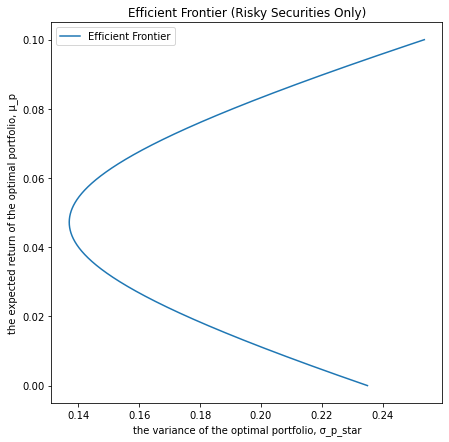
\includegraphics[width=0.6\textwidth]{Efficient Frontier Risky Only.png}
    \caption{Efficient Frontier (Risky Securities Only)}
    \label{fig:Efficient Frontier Risky Only}
\end{figure}
%%%%%%%%%%%%%%%%%%%%%%%%%%%%%%%%%%%%%%
\subsubsection{The Global Minimum Variance Portfolio}
The global minimum variance portfolio (GMV) is the portfolio that has the lowest variance out of all efficient portfolio. It's pretty crucial to our interpretation of the MVO framework and also the two fund separation theorem.

We find it by solving
$$
\frac{d \sigma_p^{*^2}}{d \mu_p}=\frac{2 A \mu_p-2 B}{\Delta} \equiv 0
$$
Therefore $A \mu_p=B$ so that $\gamma^{*}=\frac{\mu_p A-B}{\Delta}=0$ and
\begin{align}
\bm{w}_{gmv}^{*} & =\lambda^{*} \mathbf{\Sigma}^{-1} \bm{e}=\frac{C-\mu_p B}{A C-B^{2}} \mathbf{\Sigma}^{-1} \bm{e}=\frac{\mathbf{\Sigma}^{-1} \bm{e}}{\bm{e}^{\top} \mathbf{\Sigma}^{-1} \bm{e}} .
\end{align}
\begin{remark}
    We observe that $\bm{w}_{gmv}^{*}$ does not depend on the expected returns $(\bm{\mu})$ of the risky securities.
\end{remark}
\begin{figure}[!htp]
    \centering
    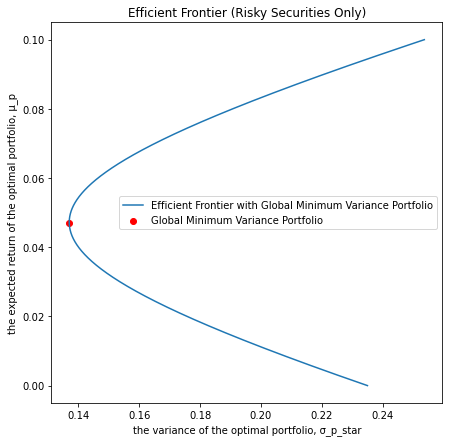
\includegraphics[width=0.6\textwidth]{Global Minimum Variance Portfolio.png}
    \caption{Efficient Frontier (Risky Securities Only) with Global Minimum Variance Portfolio}
    \label{fig:Global Minimum Variance Portfolio}
\end{figure}

\subsubsection{Two Fund Separation: Only Risky Securities}
{\color{C6}\textbf{Motivation:} We want to see if any portfolio on the efficient frontier can be represented by a linear combination of two special portfolios on the efficient frontier. That way, we can attain any efficient portfolio by investing in a combination of two special portfolios (funds). Intuitively, one of the special portfolios could be the global minimum variance portfolio $\bm{w}_{gmv}^{*}$. Now, we want to find the other one by a rather witty construction.}

Recall that for all minimum-variance portfolios where $\lambda^{*}=\lambda^{*}\left(\mu_p\right)$ and $\gamma^{*}=\gamma^{*}\left(\mu_p\right)$, we have
\begin{align*}
    w^{*}&=\lambda^{*} \mathbf{\Sigma}^{-1} \bm{e}+\gamma^{*} \mathbf{\Sigma}^{-1} \bm{\mu}\\
    &=\lambda^{*} A \bm{w}_{gmv}^{*}+\gamma^{*} \mathbf{\Sigma}^{-1} \bm{\mu}
\end{align*}
We want to rewrite $\gamma^{*} \mathbf{\Sigma}^{-1} \bm{\mu}= \gamma^{*} T\bm{w}^*_d, T\in \mathbb{R}$. Then, we must have
\[
\bm{e}^\top \bm{w}_d^{*}=1, \quad T\bm{w}^*_d = \mathbf{\Sigma}^{-1} \bm{\mu}
\]
Inspired by the look of $\bm{w}_{gmv}^{*}$, we set 
$$
\bm{w}^*_d=\frac{\mathbf{\Sigma}^{-1} \bm{\mu}}{\bm{e}^{\top} \mathbf{\Sigma}^{-1} \bm{\mu}}
$$
Then we must have 
{\color{C6}$$
\bm{w}^{*}=\lambda^{*} A \bm{w}_{gmv}^{*}+\gamma^{*} B \bm{w}^*_d
$$}
where $A=\bm{e}^{\top}\mathbf{\Sigma}^{-1} \bm{e}$ and $B=\bm{e}^{\top}\mathbf{\Sigma}^{-1}\bm{\mu}=\bm{\mu}^{\top} \mathbf{\Sigma}^{-1}\bm{e}$. 

From \cref{eq:lambda gamma MVO}, it's easy to show that $\lambda^{*} A+\gamma^{*} B =1$, which implies that any portfolio on the efficient frontier can be represented by a linear combination of $\bm{w}_{gmv}^{*}$ and $\bm{w}^*_d$.

\begin{figure}[!htp]
    \centering
    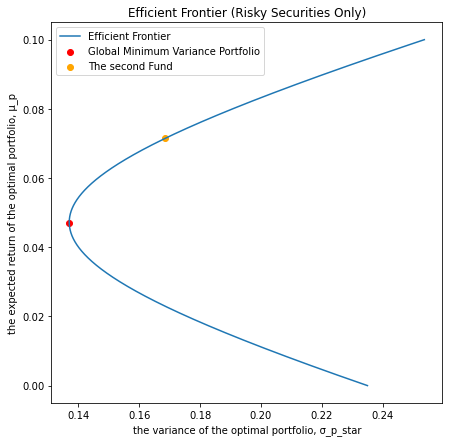
\includegraphics[width=0.6\textwidth]{Two Funds Separation Theorem.png}
    \caption{Two Funds Separation Theorem}
    \label{fig:Two Funds Separation Theorem}
\end{figure}
\begin{remark}
    Some might ask why the efficient frontier is not a line crossing the red and orange points. This is because the Two Funds Separation Theorem states that it is the weights that can be represented by a linear combination of the two funds, not the return and volatility.
\end{remark}

%%%%%%%%%%%%%%%%%%%%%%%%%%%%%%%
\subsection{MVO with Risk-free Securities}
\subsubsection{Formulation}
A risk-free asset has a return that is deterministic (that is; known as certainty). We will denote the return of the risk-less security by $r_{f}$. We observe that for the risk-less security we have
$$
r_{f}\ge 0,\quad \mathbb{E}\left[r_{f}\right] =r_{f}, \quad
\operatorname{var}\left[r_{f}\right]  =0, \quad 
\operatorname{cov}\left[r_{f}, r_{i}\right]  =0, \text { for all } i=1, \ldots, n.
$$
For the sake of incorporating in a risk-free asset, we have to change the weight constraint in the MVO framework to 
$$
w_f+\bm{w}^{\top} \bm{e}=1,
$$
where $w_f \in \mathbb{R}$ and $\bm{w} \in \mathbb{R}^n$ denote the (percentage) holdings in the risk-less and risky securities, respectively.

Then, we can start to construct the MVO problem with risk-free asset.

{\color{C6} MVO Framework with risk-free Asset:}
\begin{align*}
    \min _{\bm{w}} \quad & \frac{1}{2} \bm{w}^{\top} \mathbf{\Sigma} \bm{w} \\
    \text {s.t.} \quad   \bm{w}^{\top}\bm{\mu}+w_f r_{f} &=\mu_p, \quad  
 w_f+\bm{w}^{\top} \bm{e}=1
\end{align*}
where $\mu_p>r_{f}$ is desired level of portfolio return.

\begin{solution} Still, start with the Lagrangian
\[
L\equiv L(\bm{w}, w_f, \lambda, \gamma) = \frac{1}{2} \bm{w}^{\top} \mathbf{\Sigma} \bm{w}+\lambda(1-w_f-\bm{w}^{\top} \bm{e})+\gamma(\mu_p-\bm{w}^{\top}\bm{\mu}-w_f r_f)
\]
By the KKT condition (\cref{sec:Karush–Kuhn–Tucker (KKT) conditions}), we have
\begin{itemize}
    \item \textbf{Stationarity:} 
    \begin{align}
        \frac{\partial L}{\partial \bm{w}}&=\mathbf{\Sigma} \bm{w}-\lambda \bm{e}-\gamma \bm{\mu}=\bm{0},\label{eq:Stationarity risk free 1}\\
        \frac{\partial L}{\partial w_f}&=\lambda +\gamma r_f=0\label{eq:Stationarity risk free 2}
    \end{align}
    
    \item \textbf{Primal Feasibility:}
    \begin{align}
        \bm{w}^{\top}\bm{\mu}+w_f r_{f} &=\mu_p, \label{eq:Primal Feasibility risk free 1}\\  w_f+\bm{w}^{\top} \bm{e}&=1\label{eq:Primal Feasibility risk free 2}
    \end{align}
\end{itemize}
\begin{remark}
    Since there is no inequality constraints for such formulation, we omitted the \textbf{Dual Feasibility} condition and the \textbf{Complementary Slackness} condition. 
\end{remark}    
Now substitute $w_f$ in \cref{eq:Primal Feasibility risk free 1} using $w_f$ in \cref{eq:Primal Feasibility risk free 2}, we have
\begin{align}
    \bm{w}^{\top}(\bm{\mu}- r_f\bm{e}) =\mu_p-r_f \label{eq:riskfree i}
\end{align}
From \cref{eq:Stationarity risk free 1}, we get $\bm{w}=\mathbf{\Sigma}^{-1}(\lambda \bm{e}+\gamma \bm{\mu})$. Plug this in \cref{eq:riskfree i}, we obtain
\begin{align}
    (\lambda \bm{e}^\top+\gamma \bm{\mu}^\top)\mathbf{\Sigma}^{-1}(\bm{\mu}- r_f\bm{e}) =\mu_p-r_f \label{eq:riskfree ii}
\end{align}
From \cref{eq:Stationarity risk free 2}, we get $\lambda=-\gamma r_f$. Plug this in \cref{eq:riskfree ii}, we obtain
\begin{align}
    \gamma( \bm{\mu}^\top- r_f \bm{e}^\top)\mathbf{\Sigma}^{-1}(\bm{\mu}- r_f\bm{e}) =\mu_p-r_f \label{eq:riskfree iii}
\end{align}
Therefore, we have
\begin{align}
    \gamma^*=\frac{\mu_p-r_{f}}{\left(\bm{\mu}-r_{f} \bm{e}\right)^{\top} \mathbf{\Sigma}^{-1}\left(\bm{\mu}-r_{f} \bm{e}\right)} \label{eq:riskfree gamma}
\end{align}
We then can obtain $\bm{w}^*$ by plugging \cref{eq:Stationarity risk free 2} into $\bm{w}=\mathbf{\Sigma}^{-1}(\lambda \bm{e}+\gamma \bm{\mu})$. We have
\[
\bm{w}^*=\mathbf{\Sigma}^{-1}(-\gamma^* r_f \bm{e}+\gamma^* \bm{\mu}) = \gamma^*\mathbf{\Sigma}^{-1}(\bm{\mu}- r_f \bm{e})
\]

{\color{C6}In all, the solution to the MVO problem with risk-free security is 
\begin{align}
    \bm{w}^*=\gamma^*\mathbf{\Sigma}^{-1}(\bm{\mu}- r_f \bm{e})\label{eq:optimal weights risk free}
\end{align}
where 
\[
\gamma^*=\frac{\mu_p-r_{f}}{\left(\bm{\mu}-r_{f} \bm{e}\right)^{\top} \mathbf{\Sigma}^{-1}\left(\bm{\mu}-r_{f} \bm{e}\right)}.
\]}
\end{solution}

\subsubsection{Understanding the Optimal Allocation}
{\color{C6}\textbf{Motivation:} We want to find the relationship between $\mu_p$ and $\sigma_p=\sqrt{\bm{w}^{*^\top} \mathbf{\Sigma}\bm{w}^{*}}$ for the corresponding mean-variance efficient portfolio $\bm{w}^{*}$.}

By construction, the expected return of the optimal portfolio is
\begin{align*}
\mu_{p}&=\bm{w}^{*^\top}\bm{\mu}+\left(1-\bm{w}^{*^\top} \bm{e}\right) r_{f}\\
&=r_{f}+\bm{w}^{*^\top} (\bm{\mu}-r_f\bm{e})\\
&=r_{f}+\left(\gamma^*\mathbf{\Sigma}^{-1}(\bm{\mu}- r_f \bm{e})\right)^{\top}(\bm{\mu}-r_f\bm{e})\\
&=r_{f}+\gamma^{*}\left(\bm{\mu}-r_{f} \bm{e}\right)^{\top} \mathbf{\Sigma}^{-1}\left(\bm{\mu}-r_{f} \bm{e}\right)
\end{align*}
Some algebra shows that the variance of the optimal portfolio is
$$
\begin{aligned}
\sigma_{p}^{*^2} & =\bm{w}^{*^\top} \mathbf{\Sigma} \bm{w}^{*} \\
& =\left(\gamma^*\mathbf{\Sigma}^{-1}(\bm{\mu}- r_f \bm{e})\right)^{\top} \mathbf{\Sigma}\left(\gamma^*\mathbf{\Sigma}^{-1}(\bm{\mu}- r_f \bm{e})\right) \\
&=\gamma^{*^2}\left(\bm{\mu}-r_{f} \bm{e}\right)^{\top} \mathbf{\Sigma}^{-1}\left(\bm{\mu}-r_{f} \bm{e}\right)
\end{aligned}
$$
Since we only care about the case when $\mu_p>r_f$, we have
\[
\Longrightarrow \sigma_{p}^{*}=\gamma^{*}\sqrt{\left(\bm{\mu}-r_{f} \bm{e}\right)^{\top} \mathbf{\Sigma}^{-1}\left(\bm{\mu}-r_{f} \bm{e}\right)}
\]
{\color{C6}In all, we have
$$
\begin{cases}
    \mu_{p}&=r_{f}+\gamma^{*}\left(\bm{\mu}-r_{f} \bm{e}\right)^{\top} \mathbf{\Sigma}^{-1}\left(\bm{\mu}-r_{f} \bm{e}\right)\\
\sigma_{p}^{*}&=\gamma^{*}\sqrt{\left(\bm{\mu}-r_{f} \bm{e}\right)^{\top} \mathbf{\Sigma}^{-1}\left(\bm{\mu}-r_{f} \bm{e}\right)}
\end{cases}
$$

It's easy to see the above system gives a line that goes through point $(0, r_f)$ on the $\left(\sigma_{*}\left(\mu_p\right), \mu_p\right)$-plane:
\begin{align}
    \frac{\sigma_{p}^{*}-0}{\mu_{p} - r_f} = \frac{1}{\sqrt{\left(\bm{\mu}-r_{f} \bm{e}\right)^{\top} \mathbf{\Sigma}^{-1}\left(\bm{\mu}-r_{f} \bm{e}\right)}} = \text{constant} \label{eq:cml slope}
\end{align}}

\begin{remark}This line is now \textbf{the efficient frontier} for the MVO framework with risk-free security. (The \textbf{efficient frontier} is not the  hyperbola in this case) .
\end{remark}

%%%%%%%%%%%%%%%%%%%%
We use the risk free rate specified in \cref{eq:risk free rate}, we obtain this line as presented in \cref{fig:Capital Market Line} (We will show later that this is called the Capital Market Line.)
\begin{figure}[!htp]
    \centering
    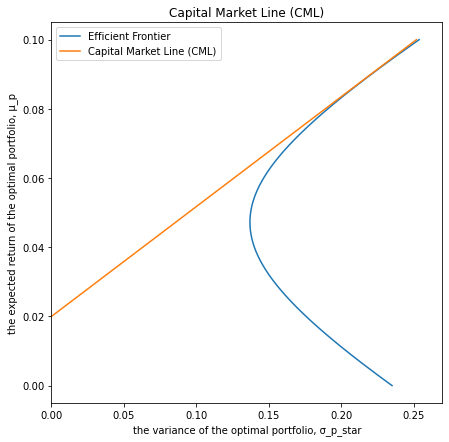
\includegraphics[width=0.6\textwidth]{Capital Market Line.png}
    \caption{Capital Market Line}
    \label{fig:Capital Market Line}
\end{figure}
%%%%%%%%%%%%%%%%%%%%

\subsubsection{Tangency Portfolio}
{\color{C6}
    Note that, given by \cref{eq:optimal weights risk free},
$$
\bm{w}^*=\gamma^* \mathbf{\Sigma}^{-1}\left(\bm{\mu}-r_{f} \cdot \bm{e}\right)
$$
implies that the weights of the risky securities of any optimal portfolio are proportional to the vector $\mathbf{\Sigma}^{-1}\left(\bm{\mu}-r_{f} \bm{e}\right)$. In other words, if we consider two optimal portfolios $\left(w_{f}^a, \bm{w}^a\right)$ and $\left(w_{f}^b, \bm{w}^b\right)$, then $\bm{w}^{a}=\kappa \bm{w}^{b}$ for some scalar $\kappa\in \mathbb{R}$.

This suggests we might want to pick an economically meaningful risky reference (benchmark) portfolio and compare all others to it.}

A canonical choice is the optimal portfolio such that $w_f=0$ (i.e. an allocation only to risky securities). This portfolio is referred to as the \textbf{tangency portfolio}.

For the tangency portfolio, we must have $\bm{e}^{\top}\bm{w}_{Tang}=1$; that is,
\[
1=\bm{e}^{\top}\bm{w}_{Tang}=\bm{e}^{\top}\gamma_{Tang}^* \mathbf{\Sigma}^{-1}\left(\bm{\mu}-r_{f} \cdot \bm{e}\right) \Longrightarrow \gamma_{Tang}^*=\frac{1}{\bm{e}^{\top} \mathbf{\Sigma}^{-1}\left(\bm{\mu}-r_{f} \bm{e}\right)}
\]
$$\Longrightarrow
\bm{w}_{Tang}=\gamma_{Tang}^*\mathbf{\Sigma}^{-1}\left(\bm{\mu}-r_{f} \cdot \bm{e}\right)=\frac{1}{\bm{e}^{\top} \mathbf{\Sigma}^{-1}\left(\bm{\mu}-r_{f} \bm{e}\right)} \cdot \mathbf{\Sigma}^{-1}\left(\bm{\mu}-r_{f} \bm{e}\right) .
$$
Hence
{\color{C6}$$
\bm{w}_{Tang}=\frac{1}{\bm{e}^{\top} \mathbf{\Sigma}^{-1}\left(\bm{\mu}-r_{f} \bm{e}\right)} \cdot \mathbf{\Sigma}^{-1}\left(\bm{\mu}-r_{f} \bm{e}\right).
$$}
The tangency is guaranteed by the fact that we only have one single solution for $\bm{w}_{Tang}$.
%%%%%%%%%%%%%%%%
\begin{figure}[!htp]
    \centering
    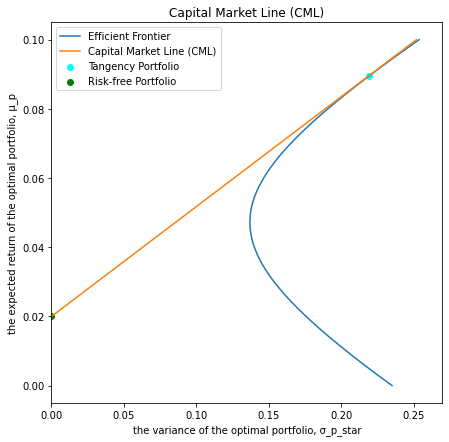
\includegraphics[width=0.6\textwidth]{CML with Tangency Portfolio.png}
    \caption{CML with Tangency Portfolio}
    \label{fig:Capital Market Line with Tangency}
\end{figure}
%%%%%%%%%%%%%%%%

\begin{proposition}\label{prop:tangency portfolio is market portfolio}
   In a one-period economy where all investors are mean-variance optimizers, everyone shares the same mean value of returns $\bm{\mu}$ and covariance matrix of asset returns $\mathbf{\Sigma}$. Furthermore, investors can borrow and lend at the risk-free rate $r_{f}$. Under these conditions, one can demonstrate that in equilibrium:
\begin{enumerate}[label=(\alph*)]
  \item the tangency portfolio consists of all securities available to investors, and
  \item each security in the tangency portfolio is held in proportion to its market value relative to the total market value of all securities.
  \end{enumerate}
  In other words, the tangency and market portfolios are the same (see \cref{def:Market Portfolio}), i.e.
$$
\bm{w}_{Tang } \equiv \bm{w}_{Market}
$$
\end{proposition}

\begin{solution}
    Since the efficient frontier for the MVO framework with a risk-free security is a straight line that goes through $(0,r_f)$ and $(\sigma_{Tang}, \mu_{Tang})$, all these mean-variance optimizers will invest in a portfolio consisting of the risk-free asset and the tangency portfolio corresponding to a point on this efficient frontier, as everyone shares the same mean value of returns $\bm{\mu}$ and covariance matrix of asset returns $\mathbf{\Sigma}$.

Suppose we have an asset $A$, and $A$ is not in the tangency portfolio. Then, by the above logic, nobody is buying $A$. Consequently, the price of $A$ will drop to the point where its expected return becomes high enough, and investors will start to include it in their portfolios, which, in this case, are the same tangency portfolio, until an equilibrium is reached. Therefore, the tangency portfolio consists of all risky securities available to investors.

Suppose the market has a total of $n$ assets $A_i$, $i=1,\ldots, n$, available to $N$ investors in total, where each investor invests $D_j$, $j=1,2,\ldots, N$ dollars in the tangency portfolio, and $\bm{w}_{Tang}=(w_{Tang}^1, \ldots, w_{Tang}^n)$, with $\bm{w}_{Tang}^\top \bm{e}=1$. Since everyone invests in the same risky portfolio (the tangency portfolio), for each asset $A_i$, its market capitalization is $C_i=\left(\sum_{j=1}^N D_j\right)w_{Tang}^i$. Then, the weight of asset $A_i$ in the market portfolio, as defined in \cref{def:Market Portfolio} (i.e., its market value relative to the total market value of all securities), is:
\[
w_M^i=\frac{C_i}{\sum_{i=1}^n C_i} =\frac{\left(\sum_{j=1}^N D_j\right)w_{Tang}^i}{\sum_{i=1}^n\left(\sum_{j=1}^N D_j\right)w_{Tang}^i} = w_{Tang}^i.
\] 
    Therefore, each security in the tangency portfolio is held in proportion to its market value relative to the total market value of all securities.

    Hence, by \cref{def:Market Portfolio}, we see that the tangency and market portfolios are the same, i.e.,
$$
\bm{w}_{Tang } \equiv \bm{w}_{Market}
$$

\end{solution}
\begin{remark}A crucial insight from the above result is that it's not that the market portfolio is determined by the MVO framework; the market portfolio simply exists in the market. It is the tangency portfolio generated under the MVO framework, under ideal conditions, that must align with the market portfolio.
\end{remark}


\begin{proposition}\label{prop: market portfolio maximize sharpe}The tangency / market portfolio can be determined by solving the maximal Sharpe ratio problem
\begin{align*}
    \max_{\bm{w}} \quad & \frac{\bm{w}^{\top} \bm{\mu}-r_{f}}{\sqrt{\bm{w}^{\top} \mathbf{\Sigma} \bm{w}}} \\
    \text {s.t.} \quad   & \bm{w}^{\top} \bm{e}=1
\end{align*}
\end{proposition}


\begin{remark}This formulation offers us a new perspective for the MVO framework with risk-free security where we are essentially maximizing the sharpe ratio.

\end{remark}

\subsubsection{The Capital Market Line (CML)}\label{sec:The Capital Market Line (CML)}
{\color{C6}\textbf{Motivation:} Since we now know that under the MVO framework with risk-free security, the efficient frontier is a straight line that passes through point $(0, r_f)$ and $(\mu_M, \sigma_M)$, we want to represent other optimal portfolio on the line as a linear combination of these two special ones.}

It immediately follows from \cref{eq:cml slope}, we get
\[
\frac{\sigma_{M}^{*}-0}{\mu_{M} - r_f} = \frac{\sigma_{p}^{*}-0}{\mu_{p} - r_f} = \frac{1}{\sqrt{\left(\bm{\mu}-r_{f} \bm{e}\right)^{\top} \mathbf{\Sigma}^{-1}\left(\bm{\mu}-r_{f} \bm{e}\right)}} = \text{constant}
\]

where $\mu_{M}=\bm{w}_{M}^{\top} \bm{\mu}$ and $\sigma_{M}=\sqrt{\bm{w}_{M}^{\top} \mathbf{\Sigma} \bm{w}_{M}}$ are the expected return and variance of the market portfolio.

Then, by simple calculation, we obtain the what's so called the capital market line (CML): 
\begin{align}
\mu_{p}=r_{f}+\sigma_{p}^*\left[\frac{\mu_{M}-r_{f}}{\sigma_{M}}\right]\label{eq:cml}
\end{align}

\begin{remark}\hfill
\begin{enumerate}
    \item The bracketed term in the CML, $\left[\frac{\mu_{M}-r_{f}}{\sigma_{M}}\right]$,is referred to as \textbf{the market price of risk}.

    Its \textbf{economic meaning} can be interpret as follows: 
    \begin{itemize}
        \item The numerator $\mu_{M}-r_{f}$ is the expected return from investing in the market above the risk-free return. It is a measure of the reward for holding the risky market portfolio rather than the risk-free security.
        \item The denominator $\sigma_{M}$ is the market risk of the market portfolio. 
    \end{itemize} 
    Thus the slope of the CML,$\left[\frac{\mu_{M}-r_{f}}{\sigma_{M}}\right]$, measures the reward per unit of market risk, determines the additional return needed to compensate for a unit change in risk.
    
    {\color{C6}In other words, the CML says that the expected return on a portfolio is equal to the risk-free rate ($r_{f}$) plus a risk premium $\left(\sigma_{p}^*\left[\frac{\mu_{M}-r_{f}}{\sigma_{M}}\right]\right)$, where the risk premium is equal to the market price of risk, $\left[\frac{\mu_{M}-r_{f}}{\sigma_{M}}\right]$, (as measured by the reward per unit of market risk) times the quantity of risk for the portfolio, $\sigma_{p}^*$, (as measured by the standard deviation of the portfolio).}
    \item The CML is the two-fund separation theorem in the case of multiple risky securities and one risk-less security. Indeed, as we can see, any efficient portfolio can be attained by a linear combination of the "risk-free portfolio" and market portfolio.
\end{enumerate}
\end{remark}

The following figure illustrates the CML. Notice the CML is a tangent line to the efficient frontier (with only risk securities) at the market/tangency portfolio.
%%%%%%%%%%%%%%%%
\begin{figure}[!htp]
    \centering
    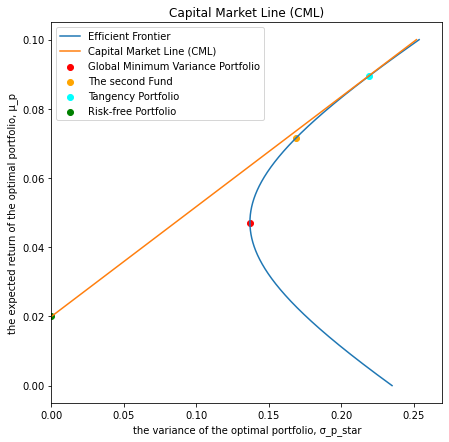
\includegraphics[width=0.6\textwidth]{All in One.png}
    \caption{MVO Summary}
    \label{fig:MVO Summary}
\end{figure}
%%%%%%%%%%%%%%%%
\begin{remark}
    \hfill
    \begin{enumerate}
        \item An investor will select a portfolio on the CML that represents a combination of borrowing or lending at the risk-free rate and the market portfolio.
        \item Portfolios to the left of the market portfolio/tangency portfolio represent combinations of risky securities and the risk-free security.
        \item Portfolios to the right of the market portfolio include purchases of risky securities made with funds borrowed at the risk-free rate. Such a portfolio is called a leveraged portfolio because it involves the use of borrowed funds.
    \end{enumerate}
\end{remark}

Finally, we present the solution to the Risk Aversion Formulation of MVO that has constraints on portfolio weights here at the end, as it is quite popular in some contexts due to its simple solution.
\begin{problem}\label{prob:The Risk Aversion Formulation}
    \textbf{(The Risk Aversion Formulation)} The risk aversion formulation is stated as
\begin{align*}
\max _{\bm{w}}\quad & \bm{w}^{\top} \bm{\mu}-\frac{\lambda}{2} \bm{w}^{\top} \mathbf{\Sigma} \bm{w} \\
& \text {s.t.} \quad 
\lambda = \lambda_0
\end{align*}
where $\lambda \geq 0$ can be interpreted as the the risk aversion coefficient specified by the investor.
\end{problem}
\begin{solution}
    Set $L(\bm{w})=\bm{w}^{\top} \bm{\mu}-\frac{\lambda_0}{2} \bm{w}^{\top} \mathbf{\Sigma} \bm{w}$. We get
    \[
    \frac{\partial L}{\partial \bm{w}} =\bm{\mu} - \lambda_0 \mathbf{\Sigma} \bm{w} \Longrightarrow \bm{w}^* = \left(\lambda_0 \mathbf{\Sigma}\right)^{-1}\bm{\mu}
    \]
    Hence, 
    \[
    \bm{w}^* = \lambda_0^{-1}\mathbf{\Sigma}^{-1}\bm{\mu}
    \]
\end{solution}
%%%%%%%%%%%%%%%%%%%%%%%%
\subsection{Drawbacks of MVO}
{\color{C6} \textbf{Motivation:} We want to know how to apply the MVO framework properly in practice as well as its advantages and disadvantages.} 

We will use the data presented in \cref{sec:Fictional Market Sample} to better illustrate our points. 

Suppose the expected returns for all countries for the next five years are 5\%. Then, according to the classical MVO framework, we obtain our portfolio weights. However, since expected returns are difficult to predict, let's consider what would happen if our views were to shift slightly. Suppose the expected return for Germany changes to 7\%, while those for France and the UK both change to 4\%. In this case, we can calculate the optimal portfolio weights using the classical MVO framework with the updated expected returns.
Then, finally, we can compare the two optimal portfolio weights as presented in the \cref{fig:MVO flaws} below:
\begin{figure}[!htp]
    \centering
    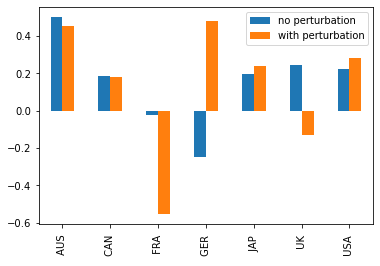
\includegraphics[width=0.5\textwidth]{MVO flaws.png}
    \caption{Optimal portfolio weights with and without perturbation}
    \label{fig:MVO flaws}
\end{figure}

We see that the weights change drastically with small perturbations, which means the classical MVO framework is not robust. On the other hand, we had significantly shorted Germany and gone long on the UK before. However, after adjusting the expected returns, we ended up going heavily long on Germany, shorting the UK, and heavily shorting France. The changes make the portfolio weights yielded by the MVO framework hard to interpret. Moreover, since we have to make estimations for the expected returns, we have no means to tackle the estimation errors, let alone the fact that it is impossible for investors to have meaningful, accurate insights for thousands of stocks currently trading in the market. Further, the classical MVO framework restricts the views to be only on the expected returns of the assets. If we want to incorporate relative views, such as stock B outperforming stock A by 5\%, we can't do that. 

Therefore, we can conclude four drawbacks of the classical MVO framework:
\begin{enumerate}
    \item The classical MVO can result in counter-intuitive portfolios.
    \item Significant impact from estimation error in expected returns and covariances.
    \item The investor is required to provide estimates of expected
returns and covariances of all assets.
    \item Hard to incorporate relative forecasts: ``B will outperform A by
0.5\% over the next month''.
\end{enumerate}



%%%%%%%%%%%%%%%%%%%%%%%%%%%%%%%%%%%%%%%%
\newpage
\section{The Capital Asset Pricing Model -- CAPM}\label{sec:capm}
{\color{C6}\textbf{Motivation:} We want to analyze how the expected rate of return of an individual asset $\mathbb{E}[r_i]$ is in relation to its individual risk $\beta_i$ with respect to the market equilibrium.}

\begin{assumption}
    \textbf{(Core Assumptions)} \begin{enumerate}[label=(\alph*)]
        \item All investors use mean-variance analysis to select a portfolio.
        \item All investors have homogeneous (same) believes about the future return, variance and covariance of assets.
        \item There is a unique risk-free rate of borrowing and lending available for all investors.
        \item There are no transaction costs.
    \end{enumerate}
\end{assumption}
Under these assumptions, as discussed in \cref{prop:tangency portfolio is market portfolio} and \cref{sec:The Capital Market Line (CML)} that an investor will select a portfolio on the CML that represents a combination of
borrowing or lending at the risk-free rate and the market portfolio..

\subsection{The Pricing Formula}
\begin{theorem}\label{theo:capm}
    \textbf{(The capital asset pricing model)} If the market portfolio $M$ is mean-variance efficient, the expected return $\mathbb{E}[r_i]$ of an asset $i$ satisfies
$$
\mathbb{E}\left[r_{i}\right]-r_{f}=\beta_{i}\left(\mathbb{E}\left[r_{M}\right]-r_{f}\right)
$$
where
\begin{itemize}
    \item $\beta_{i}=\frac{Cov\left(r_{i}, r_{M}\right)}{\sigma_{M}^{2}}$ is often called the beta of asset $i$.
    \item $\sigma_{M}^{2}$ represents the variance of the market portfolio.
\end{itemize}
\end{theorem}
\begin{solution}
Consider the portfolios spanned by individual asset $i$ and the market portfolio; that is $r_{\alpha}=\alpha r_{i}+(1-\alpha) r_{M}$ where $\alpha \in \mathbb{R}$. The expected rate of return of this portfolio is then
$$
\EE[r_{\alpha}]=\alpha \EE[r_{i}]+(1-\alpha) \EE[r_{M}]
$$
The variance of the return is
$$
\sigma_{\alpha}^{2}=\alpha^{2} \sigma_{i}^{2}+2 \alpha(1-\alpha) Cov\left(r_{i}, r_{M}\right)+(1-\alpha)^{2} \sigma_{M}^{2}
$$
As $\alpha$ varies, the values of $\left(\sigma_{\alpha}, \EE[r_{\alpha}] \right)$ trace out a curve on the $\left(\sigma, \EE[r] \right)$ diagram, as shown in the \cref{fig:capm proof} below. In particular, $\alpha=0$ corresponds to the market portfolio $M$. The curve cannot cross the capital market line, as this is the efficient frontier. Hence at $\alpha=0$ , the curve must be tangent to the capital market line at $M$, and thus having the same slope at $M$. Since from \cref{sec:The Capital Market Line (CML)}, we know the slope of the Capital Market Line is $\frac{\EE[r_M]-r_{f}}{\sigma_{M}^{2}}$, we must have

\begin{align*}
    \frac{\EE[r_M]-r_{f}}{\sigma_{M}^{2}}=\frac{\partial \EE[r_{\alpha}]}{\partial \sigma_\alpha}\Big|_{\alpha=0}\\ &= \frac{\partial \EE[r_{\alpha}]}{\partial \alpha}\frac{\partial \alpha}{\partial \sigma_\alpha}\Big|_{\alpha=0}\\
    &= \frac{\partial \EE[r_{\alpha}]}{\partial \alpha}\left(\frac{\partial \sigma_\alpha}{\partial \alpha}\right)^{-1}\Big|_{\alpha=0}\\
    &= \left(\EE[r_{i}]-\EE[r_{M}]\right)\cdot \frac{\sigma_\alpha}{\alpha \sigma_{i}^{2}+(1-2\alpha) Cov\left(r_{i}, r_{M}\right)+(\alpha-1) \sigma_{M}^{2}}\Big|_{\alpha=0}\\
    &=\frac{\EE[r_i]-\EE[r_M]}{Cov\left(r_{i}, r_{M}\right)-\sigma_{M}^{2}}
\end{align*}
Hence,
$$
\frac{\EE[r_i]-\EE[r_M]}{Cov\left(r_{i}, r_{M}\right)-\sigma_{M}^{2}}=\frac{\EE[r_M]-r_{f}}{\sigma_{M}^{2}}
$$
Solve for $\EE[r_i]$, to obtain the final result
$$
\EE[r_i] =\frac{Cov\left(r_{i}, r_{M}\right)}{\sigma_{M}^{2}}\left(\EE[r_M]-r_{f}\right) +r_{f}
$$
Set $\beta_i=\frac{Cov\left(r_{i}, r_{M}\right)}{\sigma_{M}^{2}}$, we obtain
$$
\EE[r_i]=\beta_{i}\left(\EE[r_M]-r_{f}\right) +r_{f}
$$
\end{solution}

%%%%%%%%%%%%%%%%%%%%
\begin{figure}[!htp]
    \centering
    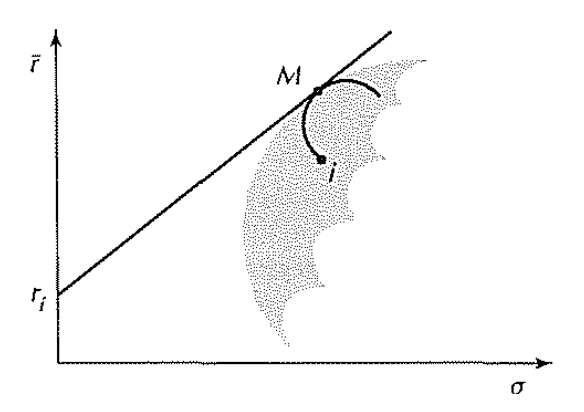
\includegraphics[width=0.5\textwidth]{capm proof.png}
    \caption{Portfolio curve: The family of portfolios traces out n curve on the diagram This curve cannot cross the \textbf{capital market line}, and hence must be tangent to that line}
    \label{fig:capm proof}
\end{figure}
%%%%%%%%%%%%%%%%%%%%

\begin{remark}\hfill
    \begin{enumerate}
        \item The CAPM model concludes that the expected excess rate of return of an asset $\EE[r_i]-r_f$ is proportional to the expected excess rate of return of the market portfolio $\EE[r_M]-r_{f}$ and the market beta $\beta_i=\frac{Cov\left(r_{i}, r_{M}\right)}{\sigma_{M}^{2}}$.
        \item The CAPM changes our concept of the risk of an asset from that of a $\sigma$ that of $\beta$. It is still true that, overall, we measure the risk of a portfolio in terms of $\sigma$, but this does not translate into a concern for the $\sigma$'s of \textbf{individual assets}. For those, the propel measure is their $\beta$'s. That is,
        \begin{align*}
            \text{ risk of a portfolio  }\quad &\longrightarrow \quad \sigma\\
            \text{ risk of an individual asset  }\quad &\longrightarrow \quad \beta
        \end{align*}
    \end{enumerate}
\end{remark}

\subsection{Understanding the CAPM Model}
To gain insight into this result, let us consider some extreme cases:
\begin{enumerate}
    \item Suppose that the asset is completely uncorrelated with the market; that is, $\beta_i=0$. Then, according to the CAPM, we have $\EE[r_i    ]=r_f$, which means that even if the asset is very risky (with large $\sigma$ ), the expected rate of return will be the risk-free rate -- there is no premium for risk. 
    
    This happens because the risk linked to an asset that doesn't move in sync with the market can be spread out or diversified. Imagine having many such assets, each one not related to the others or the market. If we bought little bits of all these assets, the overall risk or variance would be small. Because the combined return from all these assets would also have a small variance, the expected rate of return should be near $r_f$, which has no variance at all.
    \item An even more extreme case is when an asset has a negative value of $\beta_i$. In this situation, $\EE[r_i]<r_f$. This means that even if the asset has a high risk (indicated by its $\sigma$), its expected rate of return should be even lower than the risk-free rate.

This happens because such an asset actually decreases the total risk of the portfolio when it's combined with the market. So, investors are ready to accept a lower expected return due to this risk-reducing advantage. In a sense, these types of assets act like insurance. They perform well when everything else is performing poorly.
\end{enumerate}



\subsection{CAPM in Matrix-vector Form}\label{sec:CAPM in Matrix-vector Form}
Denote by $\bm{w}_{M}=\left(w_{M, 1}, \ldots, w_{M, n}\right)$ the normalized market capitalization (or benchmark) weights such that $w_{M}^{\top} \bm{e}=1$. Then the return on the market can be expressed as
$$
r_{M}=\sum_{i=1}^{n} w_{M, i} r_{i}
$$
By CAPM, the expected excess return on security $i$ becomes
$$
\begin{aligned}
\pi_{i} = \EE[r_i]-r_f = & =\beta_{i}\left(\mathbb{E}\left[r_{M}\right]-r_{f}\right) \\
& =\frac{Cov\left(r_{i}, r_{M}\right)}{\sigma_{M}^{2}}\left(\mathbb{E}\left[r_{M}\right]-r_{f}\right) \\
& =\frac{\mathbb{E}\left[r_{M}\right]-r_{f}}{\sigma_{M}^{2}} \sum_{j=1}^{n} \operatorname{cov}\left(r_{i}, r_{j}\right) w_{M, j}
\end{aligned}
$$
Defining $\delta=\frac{\mathbb{E}\left[r_{M}\right]-r_{f}}{\sigma_{M}^{2}}$, we write CAPM in the matrix-vector form
$$
\bm{\pi}=\delta \mathbf{\Sigma} \bm{w}_{M}
$$
\begin{remark}
    $\bm{\pi}$ is referred to as the ``market implied expected returns'' or ``equilibrium implied expected returns''.
\end{remark}


\subsection{Security Market Line}
The Security Market Line is nothing more than a visual representation of the CAPM formula on the $(\beta, \EE[r])$-plane or $(Cov(r,r_M), \EE[r])$-plane. 

%%%%%%%%%%%%%%%%%%%%
\begin{figure}[!htp]
    \centering
    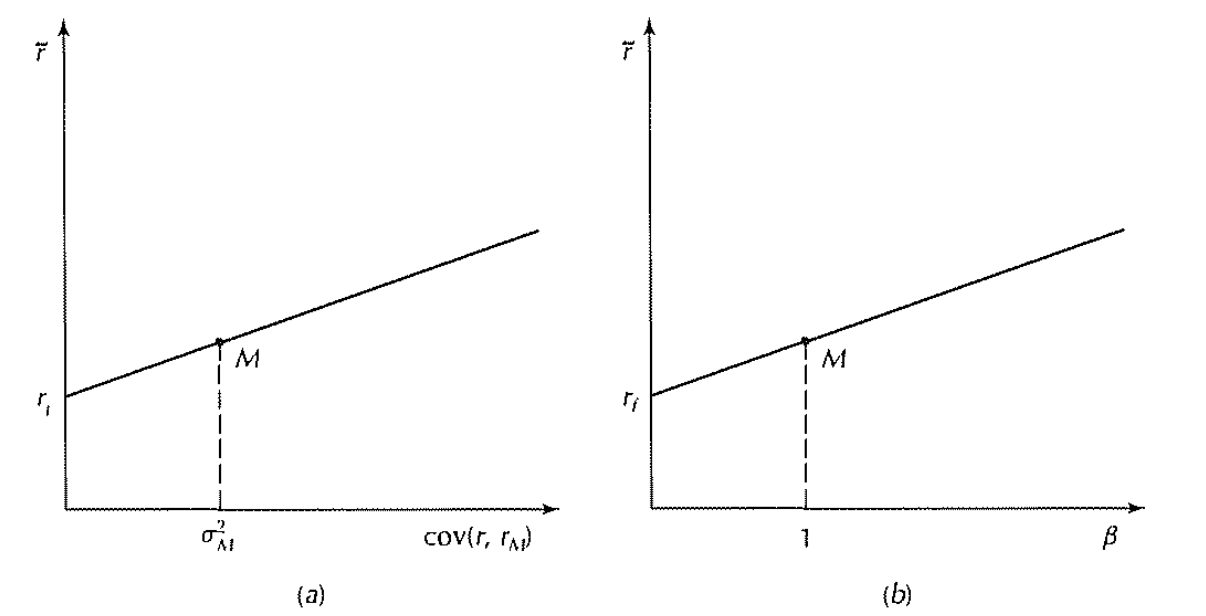
\includegraphics[width=0.8\textwidth]{security market line.png}
    \caption{Security Market Line: The expected rate of return increases linearly as the covariance with the market
increases or, equivalently, as $\beta$ increases}
    \label{fig:security market line}
\end{figure}
%%%%%%%%%%%%%%%%%%%%

\begin{remark}
    The Security Market Line highlights the essence of the CAPM formula: \textbf{Under the equilibrium conditions assumed by the CAPM, any asset should fall on the security market line. }
\end{remark}

\subsection{Systematic and Non-systematic Risks}
\begin{proposition}
    Suppose we write the return $\left(r_{i}\right)$ of asset $i$ as
    \[
r_{i}=r_{f}+\beta_{i}\left(r_M-r_{f}\right)+\varepsilon_i .
    \]
    where $r_f$ is a constant, $r_{i}, r_M$ are random variables, $\beta_i=\frac{Cov\left(r_{i}, r_{M}\right)}{\sigma_{M}^{2}}$ ,and $\varepsilon_i$ is a random variable to indicate the uncertainty in the return.
    
    Then, by CAPM, we must have
    \begin{enumerate}[label=(\alph*)]
        \item $\EE[\varepsilon_i]=0$.
        \item $Cov\left(\varepsilon_i, \sigma_{M}\right)=0$.
        \item The variance of an asset is:$$
\sigma_{i}^{2}=\beta_{i}^{2} \sigma_{M}^{2}+Var\left(\varepsilon_i\right)
$$
    \end{enumerate}
\end{proposition}
\begin{solution}
    \begin{enumerate}[label=(\alph*)]
        \item This one is trivial. We can just take the expectation on both sides, then we have our result.
        \item Since $\beta_i=\frac{Cov\left(r_{i}, r_{M}\right)}{\sigma_{M}^{2}}$ can be viewed as a constant, we have
        \begin{align*}
            Cov\left(r_i, r_M\right)&=Cov\left(r_{f}+\beta_{i}\left(r_M-r_{f}\right)+\varepsilon_i, r_M\right)\\
            &=Cov\left(\beta_{i}r_M+\varepsilon_i, r_M\right)\\
            &=Cov\left(\beta_{i}r_M, r_M\right)+Cov\left(\varepsilon_i, r_M\right)\\
            &=\beta_{i}\sigma_M^2+Cov\left(\varepsilon_i, r_M\right)\\
            &=\frac{Cov\left(r_{i}, r_{M}\right)}{\sigma_{M}^{2}}\sigma_M^2+Cov\left(\varepsilon_i, r_M\right)\\
            &=Cov\left(r_i, r_M\right)+Cov\left(\varepsilon_i, r_M\right)
        \end{align*}
        Therefore, we must have
        \[
        Cov\left(\varepsilon_i, r_M\right)=0.
        \]
        \item We have
        \begin{align*}
            Var(r_i) = \sigma_i^2 &=Var(r_{f}+\beta_{i}\left(r_M-r_{f}\right)+\varepsilon_i)\\
            &=Var(\beta_{i}r_M+\varepsilon_i)\\
            &=\beta_{i}^{2} \sigma_{M}^{2}+2\beta_i Cov(\varepsilon_i, r_M)+Var\left(\varepsilon_i\right)\\
            Cov\left(\varepsilon_i, r_M\right)=0\Longrightarrow &=\beta_{i}^{2} \sigma_{M}^{2}+Var\left(\varepsilon_i\right)
        \end{align*}
    \end{enumerate}
\end{solution}

{\color{C6}\textbf{The Key Insights are:}}

For the variance of the rate of return $r_i$ of an individual asset as represented in the form 
\begin{align}
\sigma_i^2 =\beta_{i}^{2} \sigma_{M}^{2}+Var\left(\varepsilon_i\right)\label{eq:two risks}
\end{align}
\begin{itemize}
    \item The first part $\beta_{i}^{2} \sigma_{i}^{2}$ is called \textbf{systematic risk}. This is the risk associated with the market as a whole. This risk cannot be reduced by diversification because every asset with nonzero beta contains this risk. 
    \item The second part, $Var\left(\varepsilon_i\right)$, is termed the \textbf{non-systematic}, \textbf{idiosyncratic}, or \textbf{specific risk}. This risk is uncorrelated with the market and can be reduced by diversification. 
\end{itemize}
It is the systematic (or non-diversifiable) risk, measured by beta, that is most important, since it directly combines with the systematic risk of other assets. 

\begin{remark}
    This result emphasizes that the risk of an asset is a function of its covariance with the market or, equivalently, a function of its beta.
\end{remark}

{\color{C6}\textbf{Connections with the Capital Market Line:}}

Consider an asset $r_i$ on the capital market line with a value of $\beta_i$. Then, by the equation of CML, we have
\begin{align*}
\EE[r_i]=r_{f}+\sigma_i\left[\frac{\EE[r_M]-r_{f}}{\sigma_{M}}\right]
=r_{f}+\frac{\sigma_i}{\sigma_{M}}\left(\EE[r_M]-r_{f}\right)
\end{align*}
\[
 \Longrightarrow \beta = \frac{\sigma_i}{\sigma_{M}} \Longrightarrow \sigma_i=\beta\sigma_{M}
\]
Therefore, the standard deviation of this asset is $\sigma_i=\beta \sigma_M$. Comparing this with \cref{eq:two risks}, we obtain that assets on the capital market line have only systematic risk; there is no nonsystematic risk. This asset has an expected rate of return equal to $\EE[r_i]=r_f+\beta\left(\EE[r_M]-r_f\right)$.

Now consider a whole group of other assets, all with the same value of $\beta$. According to CAPM, these all have the same expected rate of return, equal to $\EE[r_i]$. However, if these assets carry nonsystematic risk, they will not fall on the capital market line. Indeed, as the nonsystematic risk increases, the points on the $(\sigma,\EE[r])$-plane representing these assets drift to the right, as shown in \cref{fig:systematic risk} The hoizontal distance of a point from the capital market line is therefore a measure of the nonsystematic risk.

%%%%%%%%%%%%%%%%%%%%
\begin{figure}[!htp]
    \centering
    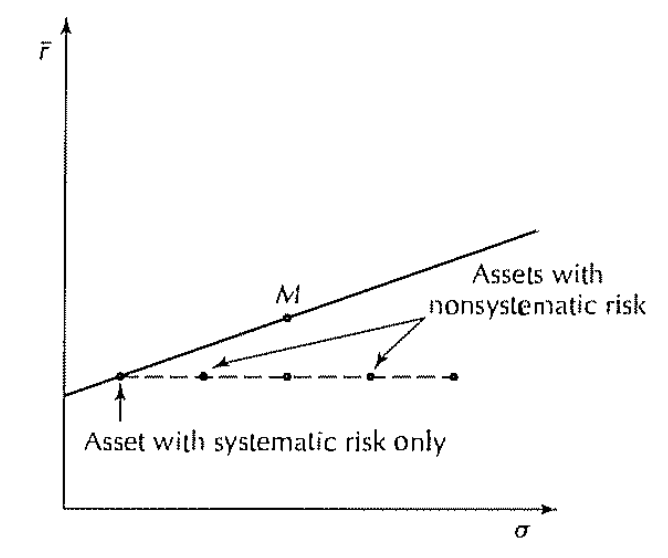
\includegraphics[width=0.5\textwidth]{systematic risk.png}
    \caption{Systematic and nonsystematic risk An asset on the \textbf{capital market line} has only systematic risk. Assets with nonsystematic risk fall to the right of the \textbf{capital market line}}
    \label{fig:systematic risk}
\end{figure}
%%%%%%%%%%%%%%%%%%%%

\subsection{Sharpe Ratio}
In the $(\sigma, \EE[r])$-plane, we can easily demonstrate the Sharpe ratio of a feasible portfolio.
\begin{figure}[!htp]
\centering
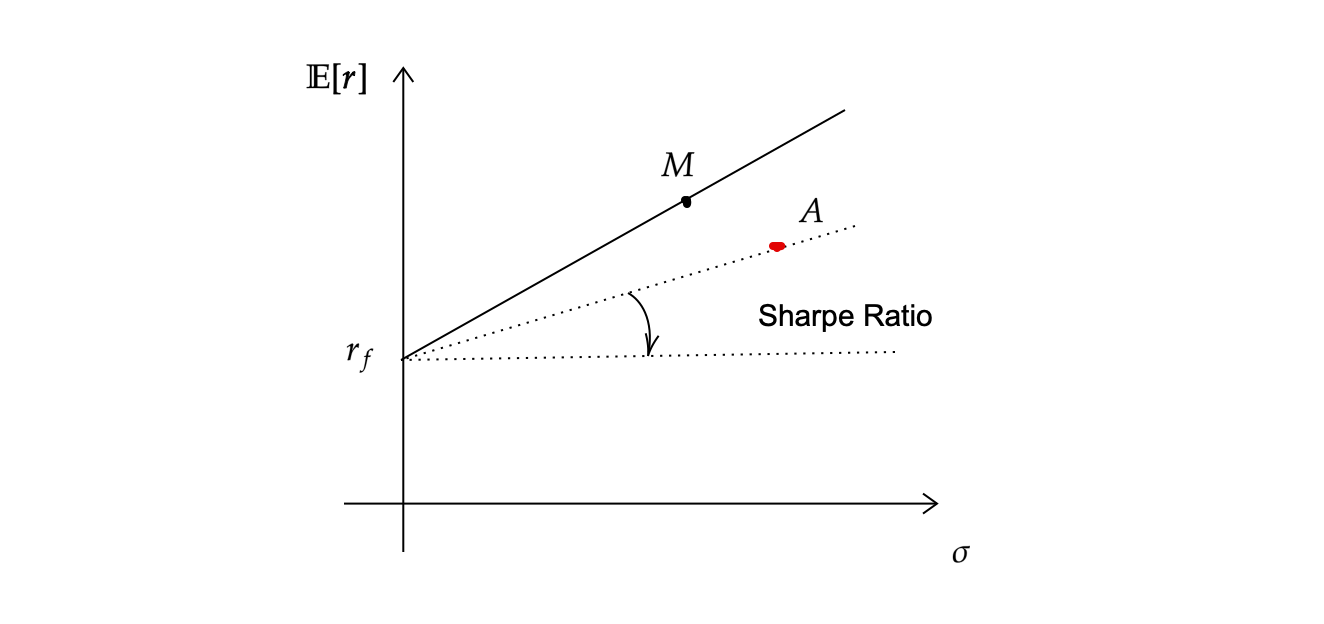
\includegraphics[width=0.8\textwidth]{sharpe ratio.png}
\caption{Sharpe Ratio}
\label{fig:sharpe ratio}
\end{figure}
From \cref{fig:sharpe ratio}, we can easily understand the intuition behind why the market portfolio is the one that maximizes the Sharpe ratio, as specified in \cref{prop: market portfolio maximize sharpe}.






%%%%%%%%%%%%%%%%%%%%%%%%%%%%%%%%%%%%%%%%
\newpage
\section{Arbitrage Pricing Theory -- Factor Model}
{\color{C6}\textbf{Motivation:} We want to generalize the CAPM model. Therefore, we can interpret the APT model as a single-period static model generalized from CAPM.}
\subsection{Formulation}
\begin{assumption}
    \textbf{(Core Assumptions)}\begin{enumerate}
        \item The average investor exhibits risk aversion  (\cref{def: Risk Preference} and non-satiation (\cref{def: Non-satiation}) preferences.
        \item Market is efficient with limited opportunity for arbitrage.
        \item Perfect capital markets
        \item Infinite number of assets
        \item Risk factors are indicative of systematic risks that cannot be diversified away and thus impact all financial assets, to some degree. Thus, these factors must be:    
Non-specific to any individual firm or industry
Compensated by the market via a risk premium
A random variable  
    \end{enumerate}
\end{assumption}
{\color{C6}\textbf{APT model Framework:}} Assume that the assumptions hold.

    Then, risky asset returns are said to follow a \textbf{factor intensity structure} if the return of each security $i(i=1, \ldots, n)$ at time $t(t=1, \ldots, T)$ can be expressed as a multifactor model:
$$
r_{i t}=\alpha_i+\beta_{i 1} f_{1 t}+\beta_{i 2} f_{2 t}+\cdots+\beta_{i k} f_{k t}+\varepsilon_{i t}=\alpha_i+\sum_{j=1}^k \beta_{i j} f_{j t}+\varepsilon_{i t}
$$
where $k \ll n<T$, $
    \mathbb{E}\left(\varepsilon_{i t}\right)=\mathbb{E}\left(f_{j t}\right)=\mathbb{E}\left(\varepsilon_{i t} f_{j t'}\right)=\mathbb{E}\left(\varepsilon_{i t} \varepsilon_{l t'}\right)=0$ $(i \neq j, i \neq l$, and for all $t, t')$ also $\mathbb{E}\left(\varepsilon_{i t}^2\right) \equiv \sigma_i^2$.
\begin{itemize}
    \item $\alpha_i$ is a constant for asset $i$,
    \item $f_{j t}$ is the $j^{th}$ factor/systematic factor/risk factor at time $t$ and can be viewed as a random variable,
    \item $\beta_{i j}$ factor beta/loading or sensitivity of the $i^{th}$ security to the $j^{th}$ factor,
    \item $\varepsilon_{i t}$ is nonsystematic (idiosyncratic) return of the $i^{th}$ security at time $t$.
\end{itemize}
\begin{remark}
    \hfill
    \begin{enumerate}
        \item We require $k \ll n$ because we don't want our matrix for betas to be rank deficient, which is essential for solving linear regression problems accurately and reliably.
        \item $\mathbb{E}[r_{i t}]=\alpha_i$.
        \item $\mathbb{E}\left(\varepsilon_{i t} \varepsilon_{l t'}\right)=0$ is often not satisfied in practice because it is impossible to find all the factors that would perfectly express the correlation between assets.
        \item Setting $k=1$ and $f_{it}=r_{Mt}-r_{ft}$, where $r_{Mt}$ and $r_{ft}$ represent the return of the market portfolio and the risk-free rate at time $t$ respectively, yields the CAPM model.
        \item A disadvantage of APT is that the selection and the number of factors to use in the model is ambiguous. Most academics use three to five factors to model returns, but the factors selected have not been empirically robust. In many instances the CAPM, as a model to estimate expected returns, has empirically outperformed the more advanced APT.
    \end{enumerate}
\end{remark}

\subsection{APT in Matrix Form}\label{sec:APT in Matrix Form}
Generalizing further and aligning with the notation often used in the linear regression context, we can re-formulate the APT model as 
$$
\bm{r}=\mathbf{X} \bm{f}+\bm{\varepsilon}, \quad \mathbb{E}[\bm{\varepsilon}]=0, \quad \mathbb{V}[\bm{\varepsilon}]=\mathbf{D}
$$
where 
\begin{itemize}
    \item $\bm{r} \in \mathbb{R}^{n}$ is an $n$-dimensional random vector containing the crosssection of \textbf{returns in excess of the risk-free rate} over some time interval $[t, t+1]$,
    \item $\mathbf{X} \in \mathbb{R}^{n\times k}$ is a (non-random) $n \times k$ matrix for factor loadings that is known before time $t$,
    \item $\bm{f} \in \mathbb{R}^{k}$ denotes a $k$-dimensional random vector process for latent factors which cannot be observed directly,
    \item $k \ll n$,
    \item $\bm{\varepsilon} \in \mathbb{R}^{n}$ is assumed to follow a mean-zero distribution with diagonal variance-covariance matrix given by $\mathbf{D}=diag\left(\sigma_1^2, \ldots, \sigma_n^2\right)$ with all $\sigma_i^2>0$.
\end{itemize}  
\begin{remark}
    Information about the $\bm{f}$-process must be obtained via statistical inference. 
\end{remark}

\begin{proposition}\label{prop:APT Useful Technique}\textbf{(APT Useful Technique)}
    \textbf{In general, it is useful} to assume that the $\bm{f}$-process is Gaussian and has finite first and second moments given by
$$
\mathbb{E}[\bm{f}]=\boldsymbol{\mu}_f, \text { and } ~\mathbb{V}[\bm{f}]=\mathbf{F}
$$
which yields
\begin{align}
    \mathbb{E}[\bm{r}]=\mathbf{X} \boldsymbol{\mu}_f, \text{ and } \mathbb{V}[\bm{r}]=\mathbf{D}+\mathbf{X} \mathbf{F} \mathbf{X}^{\top}
\end{align}
i.e.,
\[
\bm{r}\sim\mathcal{N}\left(\mathbf{X} \boldsymbol{\mu}_f, \mathbf{D}+\mathbf{X} \mathbf{F} \mathbf{X}^{\top}\right)
\]

\end{proposition}

\begin{remark}
The elements of $\boldsymbol{\mu}_f$ are called factor risk premia. 
\end{remark}

\subsection{APT model as a way to estimate covariance matrix}
Suppose the returns satisfies the APT model, then we have
$$
\bm{r}=\mathbf{X} \bm{f}+\bm{\varepsilon}, \quad \mathbb{E}[\bm{\varepsilon}]=0, \quad \mathbb{V}[\bm{\varepsilon}]=\mathbf{D}=diag\left(\sigma_1^2, \ldots, \sigma_n^2\right) \text{ with all }\sigma_i^2>0.$$
Setting $\bm{f}$ process to be Gaussian ww get $$\bm{r}\sim\mathcal{N}\left(\mathbf{X} \boldsymbol{\mu}_f, \mathbf{D}+\mathbf{X} \mathbf{F} \mathbf{X}^{\top}\right)
$$
The MVO yields:
\begin{align*}
\bm{h}^* &= \arg \max_{\bm{h}}\EE[\bm{h}^{\top}\bm{r}]-\frac{\lambda}{2}\VV[\bm{h}^\top\bm{r}]\\
&=\arg \max_{\bm{h}}\bm{h}^{\top}\mathbf{X} \boldsymbol{\mu}_f-\frac{\lambda}{2} \bm{h}^{\top}( \mathbf{X} \mathbf{F} \mathbf{X}^{\top} +\mathbf{D})\bm{h}\\
&=\arg \max_{\bm{h}}\bm{h}^{\top}\mathbf{X} \boldsymbol{\mu}_f-\frac{\lambda}{2} \bm{h}^{\top} \mathbf{X} \mathbf{F} \mathbf{X}^{\top} \bm{h}-\frac{\lambda}{2} \bm{h}^{\top} \mathbf{D} \bm{h}\\
\bm{q}:=\mathbf{X}^{\top} \bm{h}\Longrightarrow
&=\arg \max_{\bm{h}}\bm{q}^{\top} \boldsymbol{\mu}_f-\frac{\lambda}{2} \bm{q}^{\top} \mathbf{F} \bm{q}-\frac{\lambda}{2}  \bm{h}^{\top} \mathbf{D} \bm{h}
\end{align*}
and where $\lambda>0$ is the Arrow-Pratt constant absolute risk aversion. We call the third term, $\bm{h}^{\top} \mathbf{D} \bm{h}$ as  ``idiosyncratic variance''. To proceed, we want to write this term as a function of $\bm{q}$ as well.
\begin{proposition}\label{prop:APT numerical}
    An optimal portfolio $\bm{h}^*$ specified above must minimise idiosyncratic variance $\bm{h}^{\top} \mathbf{D} \bm{h}$ among all portfolios with the same exposures $\bm{q}=\mathbf{X}^{\top} \bm{h}$.
\end{proposition}

\begin{theorem}
    The risk/alpha exposures $\bm{q}^*$ and the optimal holdings $\bm{h}^*$ are
$$
\begin{aligned}
& \bm{q}^*=\lambda^{-1}\left[\mathbf{F}+\left[\mathbf{X}^{\top} \mathbf{D}^{-1} \mathbf{X}\right]^{+}\right]^{-1} \bm{\mu}_f \\
& \bm{h}^*=\lambda^{-1} \mathbf{D}^{-\frac{1}{2}}\left(\mathbf{X}^{\top} \mathbf{D}^{-\frac{1}{2}}\right)^{+}\left[\mathbf{F}+\left(\mathbf{X}^{\top} \mathbf{D}^{-1} \mathbf{X}\right)^{+}\right]^{-1} \bm{\mu}_f
\end{aligned}
$$
where $\mathbf{X}^+$ stands for the pseudo-inverse of matrix $\mathbf{X}$.
\end{theorem}
\begin{solution}
Since $\mathbf{X}^{\top} \bm{h}=\bm{q}$ and $\mathbf{D}$ is diagonal, we have
\begin{align*}
\bm{h}^*(\bm{q})
&=\arg \min_{\bm{h}} \bm{h}^{\top} \mathbf{D} \bm{h}\\
\bm{\eta}:=\mathbf{D}^{\frac{1}{2}} \bm{h} \Longrightarrow \bm{\eta}^*&=\arg\min_{\bm{\eta}}\|\bm{\eta}\|^2 \text { subject to } \mathbf{X}^{\top} \mathbf{D}^{-\frac{1}{2}} \bm{\eta}=\bm{q}
\end{align*}
This can be viewed as an ordinary least squares problem; thus, we have
$$
\bm{\eta}^*=\left(\mathbf{X}^{\top} \mathbf{D}^{-\frac{1}{2}}\right)^{+} \bm{q} \quad \Longrightarrow \quad \bm{h}^*(\bm{q})=\mathbf{D}^{-\frac{1}{2}}\left(\mathbf{X}^{\top} \mathbf{D}^{-\frac{1}{2}}\right)^{+} \bm{q}
$$
Let$
V(\bm{q})=\bm{h}^*(\bm{q})^{\top} \mathbf{D} \bm{h}^*(\bm{q})
$
be the minimum idiosyncratic variance (still subject to $\mathbf{X}^{\top} \bm{h}=\bm{q}$). Using \cref{prop:APT numerical}, the mean-variance objective can then be written entirely in terms of $\bm{q}$ :
$$
\bm{q}^* = \arg\max_{\bm{q}}\left\{\bm{q} \cdot \bm{\mu}_f-\frac{\lambda}{2}  \bm{q}^{\top} \mathbf{F} \bm{q}-\frac{\lambda}{2} \mathbf{V}(\bm{q})\right\}
$$ 

Additionally, we have 
$$
\begin{aligned}
V(\bm{q}) & =\bm{h}^*(\bm{q})^{\top} \mathbf{D} \bm{h}^*(\bm{q}) \\
& =\left[\mathbf{D}^{-\frac{1}{2}}\left(\mathbf{X}^{\top} \mathbf{D}^{-\frac{1}{2}}\right)^{+} \bm{q}\right]^{\top} \mathbf{D}\left[\mathbf{D}^{-\frac{1}{2}}\left(\mathbf{X}^{\top} \mathbf{D}^{-\frac{1}{2}}\right)^{+} \bm{q}\right] \\
& =\bm{q}^{\top}\left[\mathbf{X}^{\top} \mathbf{D}^{-1} \mathbf{X}\right]^{+} \bm{q}
\end{aligned}
$$
and therefore:
\begin{align*}
\bm{q}^* &= \arg\max_{\bm{q}}\left\{\bm{q} \cdot \bm{\mu}_f-\frac{\lambda }{2} \bm{q}^{\top} \mathbf{F} \bm{q}-\frac{\lambda }{2} V(\bm{q})\right\}\\
&= \arg\max_{\bm{q}}\left\{\bm{q} \cdot \bm{\mu}_f-\frac{\lambda }{2} \bm{q}^{\top} \mathbf{F} \bm{q}-\frac{\lambda }{2} \bm{q}^{\top}\left[\mathbf{X}^{\top} \mathbf{D}^{-1} \mathbf{X}\right]^{+} \bm{q}\right\}\\
&=\arg\max_{\bm{q}}\left\{\bm{q} \cdot \bm{\mu}_f-\frac{\lambda }{2} \bm{q}^{\top} \left[\mathbf{F}+\left[\mathbf{X}^{\top} \mathbf{D}^{-1} \mathbf{X}\right]^{+}\right]^{-1} \bm{q}\right\}\\
&=\lambda^{-1}\left[\mathbf{F}+\left[\mathbf{X}^{\top} \mathbf{D}^{-1} \mathbf{X}\right]^{+}\right]^{-1} \bm{\mu}_f
\end{align*}
and the optimal holdings $\bm{h}^*$ are 
\begin{align*}\bm{h}^*(\bm{q})
&=\mathbf{D}^{-\frac{1}{2}}\left(\mathbf{X}^{\top} \mathbf{D}^{-\frac{1}{2}}\right)^{+} \bm{q}\\
&=\lambda^{-1} \mathbf{D}^{-\frac{1}{2}}\left(\mathbf{X}^{\top} \mathbf{D}^{-\frac{1}{2}}\right)^{+}\left[\mathbf{F}+\left(\mathbf{X}^{\top} \mathbf{D}^{-1} \mathbf{X}\right)^{+}\right]^{-1} \bm{\mu}_f  
\end{align*}
\end{solution}

\begin{theorem}
    The computational complexity of the above method is $O(n)$ if $k<<n$.
\end{theorem}
\begin{solution}
    The only complicated thing involved in the above method is to compute the pseudo-inverse of $\mathbf{X}^{\top} \mathbf{D}^{-\frac{1}{2}}\in \mathbb{R}^{n\times k}$ for which we just have to compute the SVD of it where (Golub \& Van Loan 2012) showed the computational complexity is about:
$$
6 n k^2+20 k^3 \sim O(n)
$$
since $k\ll n$.
\end{solution}
\begin{remark}\hfill
\begin{enumerate}
    \item We do not assume $\mathbf{X}$ to be of full rank. Thus, this method is a good tool for handling collinearities in $\mathbf{X}$.
    \item This method is proposed in  Ritter(2016). I just present it here as a reference.
\end{enumerate}
     
\end{remark}

%%%%%%%%%%%%%%%%%%%%%%%%%%%%%%%%%%%%
\newpage
\section{Classical Black-Litterman Framework}
In the standard Mean-Variance Optimization (MVO) approach, an investor needs to estimate expected returns and covariances for all securities in their investment universe. With the sheer number of securities available today, this task is daunting. Often, investors focus on a specific area to earn better returns, which can result in a lot of estimation errors. Moreover, if an investor has more confidence in some estimates than others, it makes sense to treat these inputs differently when building portfolios. But, you can't do this in the traditional MVO approach. It's important to note that including external insights into formal models is crucial in practice. These insights can be valuable inputs, and portfolio managers might not want to hand over control to an automated system or `black box'. This is where the Black-Litterman model comes in. It's a modified MVO that allows external insights, like a portfolio manager's judgment, to be included in formal models using Bayesian techniques. It addresses the issue of estimation errors, providing a way for portfolio managers to have better control over a quantitative framework



\subsection{General Assumptions}

\begin{assumption} \textbf{(Base Assumption)}
    Unless the investor has a specific view of the security, the expected return of a security should be consistent with market equilibrium.
\end{assumption}
\begin{remark}
    In other words, an unconstrained investor who does not have any
views on the market should hold the market. (Gain beta if you can't earn alpha.)
\end{remark}


\begin{assumption}\textbf{(Core Assumptions)}\hfill
\begin{enumerate}[label=(\alph*)]
    \item Securities:
$$
\bm{r} \sim \mathcal{N}(\bm{\mu}, \mathbf{\Sigma})
$$
Security returns form a multivariate normally
distributed random
vector.
\item Market equilibrium (CAPM prior):
$$
\bm{\mu} \sim \mathcal{N}(\bm{\pi}, \tau \mathbf{\Sigma})
$$
The vector of expected return, $\bm{\mu}$, is itself a multivariate normally distributed random
vector.
\item Investor's views:
$$
\mathbf{P} \bm{\mu} \sim \mathcal{N}(\bm{q}, \mathbf{\Omega})
$$
\end{enumerate}
where
\begin{itemize}
  \item $\bm{\mu} \in \mathbb{R}^{n}$ is the vector of expected return,

  \item $\mathbf{\Sigma} \in \mathbb{R}^{n \times n}$ is the covarince matrix of returns,

  \item $\bm{\pi} \in \mathbb{R}^{n}$ is the vector of CAPM equilibrium returns (prior),

\item $0< \tau<1$, $\tau\in \mathbb{R}$ is a parameter to express the uncertainty in the CAPM equilibrium,

  \item $\bm{q} \in \mathbb{R}^{k}$ is the vector of the expected returns of investor views (forecasts /``alphas''),

  \item $\mathbf{P} \in \mathbb{R}^{k \times n}$ the matrix of investor's views, and sometimes referred to as the ``picking matrix'' as it ``picks out'' the securities that the investor has views about.

    \item $\mathbf{\Omega} \in \mathbb{R}^{k \times k}$  is the covariance matrix of the views, representing the uncertainty in the investor views. (the ``confidence'')
\end{itemize}
\end{assumption}
\begin{remark}\hfill
\begin{enumerate}
    \item Assumptions (a) and (b) encapsulate the idea that the expected returns of the securities deviate from the perceived market equilibrium. 
    \item Naturally, both the expected return vector and the vector of market equilibrium returns are not observable and have to be estimated.
\end{enumerate}
\end{remark}

{\color{C6}\textbf{Incorporate Investor's Views}}\label{subsubsec:investor's views}
\begin{example}
\textbf{(Investor's View)} Let us assume we have four assets and three views ($n=4, k=3$):
$$
\begin{aligned}
& \mathbb{E}\left[r_{1}\right]=3 \% \pm 3.9 \% \text { with } 95 \% \text { confidence }(1.96 \times 2 \%=3.92 \%) \Longleftarrow\hat{se}_1 \text { or }\sigma_1=2\%,\\
& \mathbb{E}\left[r_{2}\right]=4 \% \pm 5.9 \% \text { with } 95 \% \text { confidence }(1.96 \times 3 \%=5.88 \%)\Longleftarrow\hat{se}_2 \text { or }\sigma_2=3\%, \\
& \mathbb{E}\left[r_{4}\right]-\mathbb{E}\left[r_{3}\right]=1 \% \pm 2 \% \text { with } 95 \% \text { confidence }(1.96 \times 1 \%=1.96 \%)\Longleftarrow\hat{se}_3 \text { or }\sigma_3=1\%.
\end{aligned}
$$
We express the views as
$$
\bm{q}+\bm{\bm{\varepsilon}}=\mathbf{P} \bm{\mu} \quad \text { where } \quad \bm{\bm{\varepsilon}} \sim \mathcal{N}(0, \mathbf{\Omega})
$$
$$
\mathbf{P}=\left[\begin{array}{cccc}
1 & 0 & 0 & 0 \\
0 & 1 & 0 & 0 \\
0 & 0 & -1 & 1
\end{array}\right], \bm{q}=\left[\begin{array}{l}
3 \% \\
4 \% \\
1 \%
\end{array}\right], \quad \mathbf{\Omega}=\left[\begin{array}{ccc}
2 \%^{2} & 0 & 0 \\
0 & 3 \%^{2} & 0 \\
0 & 0 & 1 \%^{2}
\end{array}\right]
$$
\end{example}
\begin{remark}\hfill
\begin{enumerate}
    \item \textbf{(More detail)} That is, 
\[
\bm{q}+\bm{\varepsilon}=\begin{bmatrix}
3 \% \\
4 \% \\
1 \%
\end{bmatrix}+\begin{bmatrix}
\varepsilon_1 \\
\varepsilon_2 \\
\varepsilon_3 \\
\end{bmatrix}=\begin{bmatrix}
1 & 0 & 0 & 0 \\
0 & 1 & 0 & 0 \\
0 & 0 & -1 & 1
\end{bmatrix}\cdot \begin{bmatrix}
\mathbb{E}\left[r_{1}\right] \\
\mathbb{E}\left[r_{2}\right] \\
\mathbb{E}\left[r_{3}\right] \\
\mathbb{E}\left[r_{4}\right]
\end{bmatrix} = \begin{bmatrix}
\mathbb{E}\left[r_{1}\right] \\
\mathbb{E}\left[r_{2}\right] \\
\mathbb{E}\left[r_{4}\right]-\mathbb{E}\left[r_{3}\right] \\
\end{bmatrix} 
\] 
where
\[
\bm{\bm{\varepsilon}} = \begin{bmatrix}
\varepsilon_1 \\
\varepsilon_2 \\
\varepsilon_3 \\
\end{bmatrix} \sim \mathcal{N}(0, \mathbf{\Omega}), \quad \mathbf{\Omega}=\begin{bmatrix}
\sigma_1^{2} & 0 & 0 \\
0 & \sigma_2^{2} & 0 \\
0 & 0 & \sigma_3^{2}
\end{bmatrix}=\begin{bmatrix}
2 \%^{2} & 0 & 0 \\
0 & 3 \%^{2} & 0 \\
0 & 0 & 1 \%^{2}
\end{bmatrix}
\]
\item The off diagonal elements of $\mathbf{\Omega}$ are typically set to zero. This is because it is often convenient to assume (but of course not necessary) that views are uncorrelated.
\item The larger the values of the diagonal elements, the more the investor's predicted expected return can vary, and the less confidence there is in your views.
\end{enumerate}
\end{remark}

{\color{C6}\textbf{Estimate Market Equilibrium, $\bm{\pi}$}}
\begin{example}
Our starting point is CAPM. From \cref{sec:CAPM in Matrix-vector Form}, we obtain that as $\delta=\frac{\mathbb{E}\left[r_{M}\right]-r_{f}}{\sigma_{M}^{2}}$ is defined to be the ``market price of risk'', the expected excess return on security $i$  becomes
$$
\bm{\pi}=\delta \mathbf{\Sigma} \bm{w}_{M}
$$
\end{example}
\begin{remark}
   Given market capitalization weights, market price of risk and a covariance matrix

\begin{itemize}
  \item Determining $\bm{\pi}$ by calculating $\bm{\pi}=\delta \mathbf{\Sigma} w_{M}$ is called "reverse optimization"

  \item $\bm{\pi}$ is referred to as the ``market implied expected returns" or ``equilibrium implied expected returns"
\end{itemize}
\end{remark}

\subsection{Theil's Mixed Estimation Formulation}
{\color{C6}\textbf{Calculating Black-Litterman Expected Returns}}

We can rewrite assumption (b) and (c) as 
$$
\begin{aligned}
& \bm{\pi}=\bm{\mu}+\bm{\nu}, \quad \bm{\nu} \sim \mathcal{N}(\bm{0}, \tau \mathbf{\Sigma})\in \mathbb{R}^n \\
& \bm{q}=\mathbf{P} \bm{\mu}+\bm{\bm{\varepsilon}}, \quad \bm{\bm{\varepsilon}} \sim \mathcal{N}(\bm{0}, \mathbf{\Omega})\in \mathbb{R}^k
\end{aligned} \quad \Longleftrightarrow \quad \begin{bmatrix}\bm{\pi} \\
\bm{q}\end{bmatrix} = \begin{bmatrix}\mathbf{I} \\
\mathbf{P}\end{bmatrix}\bm{\mu} + \begin{bmatrix}\bm{\nu} \\
\bm{\bm{\varepsilon}}\end{bmatrix}
$$
Stacking these two equations in the form
$$
\bm{y}=\mathbf{X} \bm{\mu}+\bm{\bm{\varepsilon}}', \quad \bm{\bm{\varepsilon}}' \sim \mathcal{N}(0, \mathbf{V})
$$
where $\mathbf{I}$ denotes the $n \times n$ identity matrix, and 
$$
\bm{y}=\begin{bmatrix}\bm{\pi} \\
\bm{q}\end{bmatrix}\in \mathbb{R}^{n+k}, \quad \mathbf{X}=\begin{bmatrix}\mathbf{I} \\
\mathbf{P}\end{bmatrix}\in \mathbb{R}^{(n+k)\times n}, \quad \mathbf{V}=\begin{bmatrix}\tau \mathbf{\Sigma} & \bm{0}\\
\bm{0} & \mathbf{\Omega}\end{bmatrix}\in \mathbb{R}^{(n+k)\times (n+k)}.
$$
It's easy to see that this is just a standard linear model for the expected returns $\bm{\mu}=\mathbb{E}[\bm{r}]$ that can be solved using generalized/weighted least squares (GLS). Calculating the GLS estimator we obtain the Black-Litterman expected return
$$
\begin{aligned}
\bm{\hat{\bm{\mu}}}_{BL} & =\left(\mathbf{X}^\top \mathbf{V}^{-1} \mathbf{X}\right)^{-1} \mathbf{X}^\top \mathbf{V}^{-1} \bm{y} \\
& =\left(\begin{bmatrix}
\mathbf{I} & \mathbf{P}^\top
\end{bmatrix} \begin{bmatrix}
(\tau \mathbf{\Sigma})^{-1} & \bm{0}\\
\bm{0} & \mathbf{\Omega}^{-1}
\end{bmatrix}\begin{bmatrix}
\mathbf{I} \\
\mathbf{P}
\end{bmatrix}\right)^{-1}\begin{bmatrix}
\mathbf{I} & \mathbf{P}^\top
\end{bmatrix}\begin{bmatrix}
(\tau \mathbf{\Sigma})^{-1} & \bm{0}\\
\bm{0} & \mathbf{\Omega}^{-1}
\end{bmatrix}\begin{bmatrix}
\bm{\pi} \\
\bm{q}
\end{bmatrix} \\
& =\left(\begin{bmatrix}
\mathbf{I} & \mathbf{P}^\top
\end{bmatrix}\begin{bmatrix}
(\tau \mathbf{\Sigma})^{-1} \\
\mathbf{\Omega}^{-1} \mathbf{P}
\end{bmatrix}\right)^{-1}\begin{bmatrix}
\mathbf{I} & \mathbf{P}^\top
\end{bmatrix}\begin{bmatrix}
(\tau \mathbf{\Sigma})^{-1} \bm{\pi} \\
\mathbf{\Omega}^{-1} \bm{q}
\end{bmatrix} \\
& =\left[(\tau \mathbf{\Sigma})^{-1}+\mathbf{P}^\top \mathbf{\Omega}^{-1} \mathbf{P}\right]^{-1}\left[(\tau \mathbf{\Sigma})^{-1} \bm{\pi}+\mathbf{P}^\top \mathbf{\Omega}^{-1} \bm{q}\right] \\
\end{aligned}
$$
Therefore, we get
\[
\bm{\hat{\bm{\mu}}}_{BL} =\left[(\tau \mathbf{\Sigma})^{-1}+\mathbf{P}^\top \mathbf{\Omega}^{-1} \mathbf{P}\right]^{-1}\left[(\tau \mathbf{\Sigma})^{-1} \bm{\pi}+\mathbf{P}^\top \mathbf{\Omega}^{-1} \bm{q}\right] \in\mathbb{R}^n
\]
This is the (posterior) Black-Litterman expected returns that ``blend'' the market equilibrium with the investor's views.
\begin{remark}
    This way of calculating the Black-Litterman expected return is called the mixed estimation method of Theil and Goldberger (1961)\cite{theil_goldberger_1961}.
\end{remark}
{\color{C6}\textbf{Calculating the Covariance Matrix of Black-Litterman Expected Returns}}

To fit the Black-Litterman approach into the MVO framework, we still need the covariance matrix, $\mathbf{\Sigma}_{BL}:=\mathbb{V}[\bm{\hat{\bm{\mu}}}_{BL}]$, of Black-Litterman Expected Returns, $\bm{\hat{\bm{\mu}}}_{BL}$.

\begin{theorem} \textbf{(The Covariance Matrix
of the Black-Litterman Returns)}
The covariance (i.\bm{e}. uncertainty) of the Black-Litterman expected return
$\bm{\hat{\bm{\mu}}}_{BL}$ is 
$$
\mathbf{\Sigma}_{BL}:=\mathbb{V}\left[\bm{\hat{\bm{\mu}}}_{BL}\right]=\left[(\tau \mathbf{\Sigma})^{-1}+\mathbf{P}^\top \mathbf{\Omega}^{-1} \mathbf{P}\right]^{-1}
$$
Note that here ``$\mathbb{V}$'' stands for the covariance matrix of $\bm{\hat{\bm{\mu}}}_{BL}$.
\end{theorem}
\begin{proof}
    Since $\bm{\hat{\bm{\mu}}}_{BL} = (\mathbf{X}^T\mathbf{V}^{-1}\mathbf{X})^{-1}\mathbf{X}^T\mathbf{V}^{-1}\bm{y}$, and $\mathbf{X},\mathbf{V}$ can be viewed as constant matrices, we obtain by the definition of the covariance matrix 
\begin{align*}
    \mathbb{V}[\bm{\hat{\bm{\mu}}}_{BL}] 
    &= \mathbb{E}[(\bm{\hat{\bm{\mu}}}_{BL}-\mathbb{E}[\bm{\hat{\bm{\mu}}}_{BL}])(\bm{\hat{\bm{\mu}}}_{BL}-\mathbb{E}[\bm{\hat{\bm{\mu}}}_{BL}])^\top]\\
    &=\mathbb{E}\left[\left(\mathbf{X}^T\mathbf{V}^{-1}\mathbf{X})^{-1}\mathbf{X}^T\mathbf{V}^{-1}(\bm{y}-\mathbb{E}[\bm{y}])\right)\left((\mathbf{X}^T\mathbf{V}^{-1}\mathbf{X})^{-1}\mathbf{X}^T\mathbf{V}^{-1}(\bm{y}-\mathbb{E}[\bm{y}])\right)^\top\right]\\
    &=(\mathbf{X}^T\mathbf{V}^{-1}\mathbf{X})^{-1}\mathbf{X}^T\mathbf{V}^{-1}\mathbb{E}[(\bm{y}-\mathbb{E}[\bm{y}])(\bm{y}-\mathbb{E}[\bm{y}])^\top]\Big((\mathbf{X}^T\mathbf{V}^{-1}\mathbf{X})^{-1}\mathbf{X}^T\mathbf{V}^{-1}\Big)^T\\
    &=(\mathbf{X}^T\mathbf{V}^{-1}\mathbf{X})^{-1}\mathbf{X}^T\mathbf{V}^{-1}\mathbb{V}[\bm{y}]\Big((\mathbf{X}^T\mathbf{V}^{-1}\mathbf{X})^{-1}\mathbf{X}^T\mathbf{V}^{-1}\Big)^T\\
    \mathbb{V}[\bm{y}] =\mathbf{V} \Longrightarrow&= (\mathbf{X}^T\mathbf{V}^{-1}\mathbf{X})^{-1}\mathbf{X}^T\mathbf{V}^{-1}\mathbf{V}\Big((\mathbf{X}^T\mathbf{V}^{-1}\mathbf{X})^{-1}\mathbf{X}^T\mathbf{V}^{-1}\Big)^T\\
    \mathbf{V}^\top =\mathbf{V} \Longrightarrow&= (\mathbf{X}^T\mathbf{V}^{-1}\mathbf{X})^{-1}\mathbf{X}^T\mathbf{V}^{-1}\mathbf{V}\mathbf{V}^{-1}XX^{-1}\mathbf{V}(\mathbf{X}^T)^{-1}\\
    &=(\mathbf{X}^T\mathbf{V}^{-1}\mathbf{X})^{-1} \\
    &= [(\tau \mathbf{\Sigma})^{-1} + \mathbf{P}^T\mathbf{\Omega}^{-1}\mathbf{P}]^{-1}
\end{align*}

Hence, we have 
\[
\mathbf{\Sigma}_{\mathbf{B} L}:=\mathbb{V}[\bm{\hat{\bm{\mu}}}_{BL}] = [(\tau \mathbf{\Sigma})^{-1} + \mathbf{P}^T\mathbf{\Omega}^{-1}\mathbf{P}]^{-1}.
\]
\end{proof}

{\color{C6}\textbf{Calculating the portfolio weights under the Black-Litterman framework}}

Under the Black-Litterman model, the Black-Litterman expected returns generated by assumption (b) and (c) is  $\bm{\mu}_{BL}$. Since assumption (a) specifies that $\bm{r} \sim \mathcal{N}\left(\bm{\mu}, \mathbf{\Sigma}\right)$, we can write $\bm{r}$ as $\bm{r} = \bm{\hat{\bm{\mu}}}_{\mathbf{B} L} + \bm{\xi}$ where $\bm{\xi} \sim \mathcal{N}\left(\bm{0}, \mathbf{\Sigma}\right)$. Then we have $\mathbb{V}[\bm{r}] = \mathbb{V}[\bm{\hat{\bm{\mu}}}_{\mathbf{B} L}] + \mathbb{V}[\bm{\xi}] = \mathbf{\Sigma}_{BL}+\mathbf{\Sigma}$. That is,
$$\bm{r} \sim \mathcal{N}\left(\bm{\hat{\bm{\mu}}}_{\mathbf{B} L}, \mathbf{\Sigma}+\mathbf{\Sigma}_{\mathbf{B} L}\right)$$
We just plug in the covariance matrix, $\mathbb{V}[\bm{r}] = \mathbf{\Sigma}_{BL}+\mathbf{\Sigma}$, and the Black-Litterman Expected Returns, $\bm{\hat{\bm{\mu}}}_{BL}$, to the classical MVO framework to get our optimal $\bm{w}^*$.
$$\bm{w}^*=\arg
\min_{\bm{w}}\left\{\bm{w}^\top \bm{\hat{\bm{\mu}}}_{BL}-\frac{\lambda}{2}\bm{w}^\top \mathbb{V}[\bm{r}]\bm{w} \right\}= \lambda^{-1}(\mathbf{\Sigma}_{BL}+\mathbf{\Sigma})^{-1}\bm{\hat{\bm{\mu}}}_{BL}
$$
\begin{remark}
Moreover, we have
$$
\begin{aligned}
\mathbb{V}[\bm{r}] & =\mathbf{\Sigma}+\mathbf{\Sigma}_{\mathbf{B} L} \\
& =\mathbf{\Sigma}+\left[(\tau \mathbf{\Sigma})^{-1}+\mathbf{P}^{\top} \mathbf{\Omega}^{-1} \mathbf{P}\right]^{-1} \\
\cref{coro:black-Litterman Matrix Result} \Longrightarrow& =\mathbf{\Sigma}+\tau \mathbf{\Sigma}-\tau \mathbf{\Sigma} \mathbf{P}^\top (\mathbf{\Omega}+\mathbf{P}\tau \mathbf{\Sigma} \mathbf{P}^\top)^{-1} \mathbf{P} \tau \mathbf{\Sigma}\\
&=(1+\tau) \mathbf{\Sigma}-\tau^{2} \mathbf{\Sigma} \mathbf{P}^{\top}\left[\mathbf{P} \tau \mathbf{\Sigma} \mathbf{P}^{\top}+\mathbf{\Omega}\right]^{-1} \mathbf{P} \mathbf{\Sigma}
\end{aligned}
$$
It's easy to see that 
\begin{itemize}
\item $\mathbb{V}[\bm{r}]>\mathbf{\Sigma}$ and $\mathbb{V}[\bm{r}]>\mathbf{\Sigma}_{\mathbf{B} L}$
    \item $\tau=0$ (no estimation risk) then $\mathbb{V}[\bm{r}] \equiv \mathbf{\Sigma}$
  \item $\mathbf{\Omega} \rightarrow \infty$ (uninformative prior) then $\mathbf{\Sigma}_{\mathbf{B} L} \equiv(1+\tau) \mathbf{\Sigma}$

  \item Note that if $\mathbf{\Omega}=\alpha \cdot \mathbf{P} \tau \mathbf{\Sigma} \mathbf{P}^{\top}$ (with $\mathrm{\mathbf{P}}$ full rank) then $\mathbb{V}[\bm{r}]\equiv\left(1+\tau-\frac{\tau}{1+\alpha}\right) \mathbf{\Sigma}$
\end{itemize}
\end{remark}

\subsection{Bayesian Formulation}
We derive it as in  \cref{sec:Bayesian Statistical Model}.
\begin{enumerate}[label=(\alph*)]
    \item Set parameter $\bm{\theta}=\EE[r]$, and
\[
\bm{r} \sim \mathcal{N}(\bm{\theta}, \mathbf{\Sigma})
\]
Note that this can be viewed as $\bm{r}=\bm{\theta}+\bm{\varepsilon}$ where $\bm{\varepsilon}\sim \mathcal{N}(\bm{0}, \mathbf{\Sigma})$.
\item Set prior $\pi(\bm{\theta})\sim \mathcal{N}(\bm{\pi}, \mathbf{C})$, where $\bm{\pi}=\delta \mathbf{\Sigma}\bm{w}_M$ is the market implied expected return. That is,
\[
\pi(\bm{\theta})=\exp\left[-\frac{1}{2}(\bm{\theta}-\bm{\pi})^\top\mathbf{C}^{-1}(\bm{\theta}-\bm{\pi})\right]
\]
\item The view function is given by $\mathbf{P}\bm{\theta} = \bm{q}+\bm{\nu}$ where $\bm{\nu}\sim  \mathcal{N}(0, \mathbf{\Omega})$. Then we have $\bm{q}|\bm{\theta}\sim \mathcal{N}(\mathbf{P}\bm{\theta}, \mathbf{\Omega})$, and the likelihood function is 
\[
f(\bm{q}|\bm{\theta}) = \exp\left[-\frac{1}{2}(\bm{q}-\mathbf{P}\bm{\theta})^\top\mathbf{\Omega}^{-1}(\bm{q}-\mathbf{P}\bm{\theta})\right]
\]
\end{enumerate}
\begin{solution}
Then, under the Bayesian framework, we have
\begin{align*}
    p(\bm{\theta}|\bm{q}) &=f(\bm{q}|\bm{\theta})\pi(\bm{\theta})\\
    &= \exp\left[-\frac{1}{2}(\bm{q}-\mathbf{P}\bm{\theta})^\top\mathbf{\Omega}^{-1}(\bm{q}-\mathbf{P}\bm{\theta})\right]\cdot \exp\left[-\frac{1}{2}(\bm{\theta}-\bm{\pi})^\top\mathbf{C}^{-1}(\bm{\theta}-\bm{\pi})\right]\\
    &=\exp\left[-\frac{1}{2}\left(\bm{\theta}^\top (\mathbf{P}\mathbf{\Omega}^{-1}\mathbf{P}+\mathbf{C}^{-1})\bm{\theta}-2(\bm{q}^\top\mathbf{\Omega}^{-1}\mathbf{P}+\bm{\pi}^\top \mathbf{C}^{-1} )\bm{\theta}\right)\right]
\end{align*}
\[
\Longrightarrow -2\log p(\bm{\theta}|\bm{q}) = \bm{\theta}^\top (\mathbf{P}\mathbf{\Omega}^{-1}\mathbf{P}+\mathbf{C}^{-1})\bm{\theta}-2(\bm{q}^\top\mathbf{\Omega}^{-1}\mathbf{P}+\bm{\pi}^\top \mathbf{C}^{-1} )\bm{\theta}
\]
Since the likelihood $f(\bm{q}|\bm{\theta})$ is normal and the prior $\pi(\bm{\theta})$ is also normal, which is a conjugate prior for that likelihood, it implies that the posterior is of the same family, i.e., $\bm{\theta}|\bm{q}$ is also normally distributed.

Set $\mathbf{M}=(\mathbf{P}\mathbf{\Omega}^{-1}\mathbf{P}+\mathbf{C}^{-1})$ and $\bm{u}^\top=(\bm{q}^\top\mathbf{\Omega}^{-1}\mathbf{P}+\bm{\pi}^\top \mathbf{C}^{-1} )$ in \cref{theo:A Useful Theorem}, we have
\[
\VV[\bm{\theta}|\bm{q}]=(\mathbf{P}\mathbf{\Omega}^{-1}\mathbf{P}+\mathbf{C}^{-1})^{-1}, \quad \EE[\bm{\theta}|\bm{q}]=(\mathbf{P}\mathbf{\Omega}^{-1}\mathbf{P}+\mathbf{C}^{-1})^{-1}(\mathbf{P}^\top \mathbf{\Omega}^{-1}\bm{q}+\mathbf{C}^{-1}\bm{\pi}  )
\]
Therefore, we obtain
\[\begin{cases}
\EE[\bm{r}|\bm{q}] = \EE[\bm{\theta}|\bm{q}] =  (\mathbf{P}\mathbf{\Omega}^{-1}\mathbf{P}+\mathbf{C}^{-1})^{-1}(\mathbf{P}^\top \mathbf{\Omega}^{-1}\bm{q}+\mathbf{C}^{-1}\bm{\pi}  ), \\
\VV[\bm{r}|\bm{q}] = \VV[\bm{\theta}|\bm{q}] +\VV[\bm{\varepsilon}|\bm{q}] =   (\mathbf{P}\mathbf{\Omega}^{-1}\mathbf{P}+\mathbf{C}^{-1})^{-1}+\mathbf{\Sigma}
\end{cases}
\]
We just plug in the covariance matrix, $\VV[\bm{\varepsilon}|\bm{q}]$, and the Black-Litterman Expected Returns, $\EE[\bm{r}|\bm{q}]$, to the classical MVO framework to get our optimal $\bm{w}^*$.
$$\bm{w}^*=\arg
\min_{\bm{w}}\left\{\bm{w}^\top \EE[\bm{r}|\bm{q}]-\frac{\lambda}{2}\bm{w}^\top \VV[\bm{\varepsilon}|\bm{q}]\bm{w} \right\}
$$
From \cref{prob:The Risk Aversion Formulation}, we get that the optimal portfolio is then given by
$$
\bm{w}^*=\lambda^{-1}\left[(\mathbf{P}\mathbf{\Omega}^{-1}\mathbf{P}+\mathbf{C}^{-1})^{-1}+\mathbf{\Sigma}\right]^{-1} (\mathbf{P}\mathbf{\Omega}^{-1}\mathbf{P}+\mathbf{C}^{-1})^{-1}(\mathbf{P}^\top \mathbf{\Omega}^{-1}\bm{q}+\mathbf{C}^{-1}\bm{\pi}  ) 
$$
Specifically, choose $\mathbf{C}=\tau\mathbf{\Sigma}$, we recover the classical BL model.
\end{solution}


\subsubsection{Roadmap of the Black-Litterman Framework}
Now, we can present a clear and concise illustration of the Black-Litterman framework in the image provided below.

\begin{figure}[!htp]
    \centering
    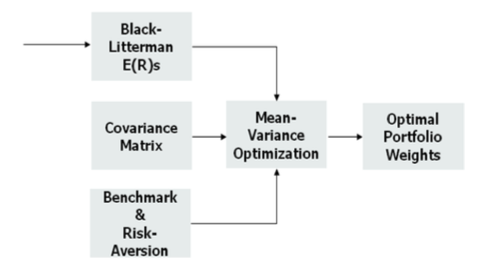
\includegraphics{black_litterman.png}
    \caption{Roadmap of the Black-Litterman model}
    \label{fig:roadmap for Black-Litterman model}
\end{figure}

\subsection{Some Properties of the Black-Litterman Model}
In this section, we examine various properties of the Black-Litterman model to gain deeper insights and uncover the implications suggested by the model, ultimately leading to a better understanding of the Black-Litterman framework.

\begin{property} \textbf{(Absence of Views)}
    If the
investor has no views (i.\bm{e}.
$\bm{q} = \bm{0}, k=0$) or the confidence in the views is zero (i.\bm{e}. $\mathbf{\Omega}\to \infty$), then the Black-Litterman returns are equal to the
equilibrium returns, i.\bm{e}. $\bm{\hat{\bm{\mu}}}_{\mathbf{B} L}=\bm{\pi}$. 
\end{property}
\begin{proof}
    This is relatively easy to prove. 
    \begin{enumerate}[label=(\alph*)]
        \item If $\bm{q} = \bm{0}, k=0$, then we have
        \[
        \bm{\hat{\bm{\mu}}}_{BL} =\left[(\tau \mathbf{\Sigma})^{-1}\right]^{-1}(\tau \mathbf{\Sigma})^{-1} \bm{\pi} =\bm{\pi}
        \]
        \item If $\mathbf{\Omega}\to \infty$, we get
        \[
        \bm{\hat{\bm{\mu}}}_{BL}=\left[(\tau \mathbf{\Sigma})^{-1}+\mathbf{P}^\top \mathbf{\Omega}^{-1} \mathbf{P}\right]^{-1}\left[(\tau \mathbf{\Sigma})^{-1} \bm{\pi}+\mathbf{P}^\top \mathbf{\Omega}^{-1} \bm{q}\right] =\left[(\tau \mathbf{\Sigma})^{-1}\right]^{-1}(\tau \mathbf{\Sigma})^{-1} \bm{\pi} =\bm{\pi}
        \]
    \end{enumerate}
\end{proof}
\begin{remark}
    \textbf{(Interpretation)} \hfill 
    \begin{enumerate}
        \item Consequently, with no views ($\bm{q}=\bm{0}$) or views with of zero confidence ($\mathbf{\Omega}\to \infty$), the investor will end up holding the market portfolio. In other words, the optimal portfolio in the absence of views is the defined market.
    \end{enumerate}
\end{remark}

\begin{property}\textbf{(``Confidence'' Weighted Expected Return)}
We can rewrite the Black-Litterman expected returns in the form
\begin{align*}
\bm{\hat{\bm{\mu}}}_{BL}&=\left[(\tau \mathbf{\Sigma})^{-1}+\mathbf{P}^{\top} \mathbf{\Omega}^{-1} \mathbf{P}\right]^{-1}\left[(\tau \mathbf{\Sigma})^{-1} \bm{\pi}+\mathbf{P}^{\top} \mathbf{\Omega}^{-1} \mathbf{P} \bm{\hat{\bm{\mu}}}_{\text{investor}}\right]\\
&= w_{\bm{\pi}}\bm{\pi} + w_{\bm{q}}\bm{\hat{\bm{\mu}}}_{\text{investor}}
\end{align*}
where the two weighting matrices are given by
$$
\begin{aligned}
& w_{\bm{\pi}}=\left[(\tau \mathbf{\Sigma})^{-1}+\mathbf{P}^{\top} \mathbf{\Omega}^{-1} \mathbf{P}\right]^{-1}(\tau \mathbf{\Sigma})^{-1} \\
& w_{\bm{q}}=\left[(\tau \mathbf{\Sigma})^{-1}+\mathbf{P}^{\top} \mathbf{\Omega}^{-1} \mathbf{P}\right]^{-1} \mathbf{P}^{\top} \mathbf{\Omega}^{-1} \mathbf{P}
\end{aligned} \quad \Longrightarrow \quad w_{\bm{\pi}}+w_{\bm{q}}=\mathbf{I} \in \mathbb{R}^{n\times n}
$$
\end{property}
\begin{proof}
    By using $\bm{q}=\mathbf{P} \bm{\mu}+\bm{\bm{\varepsilon}}$, we have that the investor's views alone imply the estimate of expected returns 
    \[\bm{\hat{\bm{\mu}}}_{\text{investor}}=\left(\mathbf{P}^{\top} \mathbf{P}\right)^{-1} \mathbf{P}^\top \bm{q}.
    \] 
    Since $\mathbf{P}\left(\mathbf{P}^{\top} \mathbf{P}\right)^{-1} \mathbf{P}^{\top}=\mathbf{I}$ where $\mathbf{I}$ is the identity matrix, we must have $\mathbf{P}\bm{\hat{\bm{\mu}}}_{\text{investor}}=\bm{q}$. Therefore, we have 
    \begin{align*}
    \bm{\hat{\bm{\mu}}}_{BL}&=\left[(\tau \mathbf{\Sigma})^{-1}+\mathbf{P}^{\top} \mathbf{\Omega}^{-1} \mathbf{P}\right]^{-1}\left[(\tau \mathbf{\Sigma})^{-1} \bm{\pi}+\mathbf{P}^{\top} \mathbf{\Omega}^{-1} \bm{q}\right]\\
    &=\left[(\tau \mathbf{\Sigma})^{-1}+\mathbf{P}^{\top} \mathbf{\Omega}^{-1} \mathbf{P}\right]^{-1}\left[(\tau \mathbf{\Sigma})^{-1} \bm{\pi}+\mathbf{P}^{\top} \mathbf{\Omega}^{-1} \mathbf{P} \bm{\hat{\bm{\mu}}}_{\text{investor}}\right]
    \end{align*}
\end{proof}
\begin{remark}\textbf{(Interpretation:)}\hfill
\begin{enumerate}
    \item Notice, $\bm{\hat{\bm{\mu}}}_{\text{investor}}$ and $\bm{\hat{\bm{\mu}}}_{BL}$ are different.
    \item We see that the Black-Litterman expected return, $\bm{\hat{\bm{\mu}}}_{BL}= w_{\bm{\pi}}\bm{\pi} +w_{\bm{q}}\bm{\hat{\bm{\mu}}}_{\text{investor}}$, is a "confidence weighted" linear combination (or ``weighted average'')of market equilibrium $\bm{\pi}$ and the expected return $\bm{\hat{\bm{\mu}}}_{\text{investor}}$ implied by the investor's views.
    \item In particular, $(\tau \mathbf{\Sigma})^{-1}$ and $\mathbf{P}^{\top} \mathbf{\Omega}^{-1} \mathbf{P}$ represent the {\color{C6}\textbf{confidence}} we have in our estimates of the market equilibrium and the views, respectively. 
    
    Therefore, if we have low confidence in the views, the resulting expected returns will be close to the ones implied by market equilibrium --- $\bm{\pi}$. Conversely, with higher confidence in the views, the resulting expected returns will deviate from the market and be close to investor's views --- $\bm{q}$.
\end{enumerate}
\end{remark}

\begin{property}\textbf{(Deviation from Market Equilibrium)}
    The Black-Litterman expected return $\bm{\hat{\bm{\mu}}}_{BL}$ can be rewritten as 
    \[
    \bm{\hat{\bm{\mu}}}_{BL}=\bm{\pi}+\tau \mathbf{\Sigma} \mathbf{P}^\top\left[\mathbf{P} \tau \mathbf{\Sigma} \mathbf{P}^\top+\mathbf{\Omega}\right]^{-1}[\bm{q}-\mathbf{P} \bm{\pi}]
    \]
\end{property}
\begin{proof}
Set $\mathbf{A}=\mathbf{\Omega}$ and $\mathbf{B}=\mathbf{P} \tau \mathbf{\Sigma} \mathbf{P}^T$ in \cref{lemma:inverse matrix sum}, we get
\begin{align*}
    (\mathbf{\Omega}+\mathbf{P}\tau \mathbf{\Sigma} \mathbf{P}^\top)^{-1} &= \mathbf{\Omega}^{-1}\left(\mathbf{\mathbf{I}}+\mathbf{P}\tau \mathbf{\Sigma} \mathbf{P}^\top \mathbf{\Omega}^{-1}\right)^{-1}\\
    \Longrightarrow (\mathbf{\Omega}+\mathbf{P}\tau \mathbf{\Sigma} \mathbf{P}^\top)^{-1}\left(\mathbf{\mathbf{I}}+\mathbf{P}\tau \mathbf{\Sigma} \mathbf{P}^\top \mathbf{\Omega}^{-1}\right) &= \mathbf{\Omega}^{-1}
    \end{align*}
    \begin{align}
    \Longrightarrow (\mathbf{\Omega}+\mathbf{P}\tau \mathbf{\Sigma} \mathbf{P}^\top)^{-1}&= \mathbf{\Omega}^{-1}-(\mathbf{\Omega}+\mathbf{P}\tau \mathbf{\Sigma} \mathbf{P}^\top)^{-1}\mathbf{P}\tau \mathbf{\Sigma} \mathbf{P}^\top \mathbf{\Omega}^{-1}\label{eq:eq 3}
\end{align}

Plug the result from   \cref{coro:black-Litterman Matrix Result} into the formula for $\bm{\hat{\bm{\mu}}}_{BL}$, we have
\begin{align*}
\bm{\hat{\bm{\mu}}}_{BL}
&=[(\tau \mathbf{\Sigma})^{-1}+\mathbf{P}^T\mathbf{\Omega}^{-1}\mathbf{P}]^{-1}[(\tau \mathbf{\Sigma})^{-1}\bm{\pi} + \mathbf{P}^T\mathbf{\Omega}^{-1}\bm{q}]\\
&=\left(\tau \mathbf{\Sigma}-\tau \mathbf{\Sigma} \mathbf{P}^\top (\mathbf{\Omega}+\mathbf{P}\tau \mathbf{\Sigma} \mathbf{P}^\top)^{-1} \mathbf{P} \tau \mathbf{\Sigma} \right)[(\tau \mathbf{\Sigma})^{-1}\bm{\pi} + \mathbf{P}^T\mathbf{\Omega}^{-1}\bm{q}]\\
&=\bm{\pi} - \tau \mathbf{\Sigma} \mathbf{P}^T(\mathbf{\Omega}+\mathbf{P}\tau \mathbf{\Sigma} \mathbf{P}^\top)^{-1}\mathbf{P}\bm{\pi}+ \tau \mathbf{\Sigma} \mathbf{P}^T\mathbf{\Omega}^{-1}\bm{q}\\
&\quad - \tau \mathbf{\Sigma} \mathbf{P}^\top (\mathbf{\Omega}+\mathbf{P}\tau \mathbf{\Sigma} \mathbf{P}^\top)^{-1} \mathbf{P} \tau \mathbf{\Sigma} \mathbf{P}^T\mathbf{\Omega}^{-1}\bm{q}\\
&=\bm{\pi} - \tau \mathbf{\Sigma} \mathbf{P}^T(\mathbf{\Omega}+\mathbf{P}\tau \mathbf{\Sigma} \mathbf{P}^\top)^{-1}\mathbf{P}\bm{\pi}\\
&\quad + \tau \mathbf{\Sigma} \mathbf{P}^T\left(\mathbf{\Omega}^{-1}-(\mathbf{\Omega}+\mathbf{P}\tau \mathbf{\Sigma} \mathbf{P}^\top)^{-1} \mathbf{P} \tau \mathbf{\Sigma} \mathbf{P}^T\mathbf{\Omega}^{-1}\right)\bm{q} \\
\cref{eq:eq 3}\Longrightarrow &=\bm{\pi} - \tau \mathbf{\Sigma} \mathbf{P}^T(\mathbf{\Omega}+\mathbf{P}\tau \mathbf{\Sigma} \mathbf{P}^\top)^{-1}\mathbf{P}\bm{\pi}+ \tau \mathbf{\Sigma} \mathbf{P}^T(\mathbf{\Omega}+\mathbf{P}\tau \mathbf{\Sigma} \mathbf{P}^\top)^{-1}\bm{q} \\
&=\bm{\pi}+\tau\mathbf{\Sigma} \mathbf{P}^T(\mathbf{\Omega}+\mathbf{P}\tau \mathbf{\Sigma} \mathbf{P}^\top)^{-1}[\bm{q}-\mathbf{P}\bm{\pi}]
\end{align*}
Therefore, we have
\[
\bm{\hat{\bm{\mu}}}_{BL}=\bm{\pi}+\tau \mathbf{\Sigma} \mathbf{P}^\top\left[\mathbf{P} \tau \mathbf{\Sigma} \mathbf{P}^\top+\mathbf{\Omega}\right]^{-1}[\bm{q}-\mathbf{P} \bm{\pi}]
\]
\end{proof}

\begin{remark}
    \textbf{(Interpretation:)} The Black-Litterman expected return $\bm{\hat{\bm{\mu}}}_{BL}$ ``tilts'' away  from the market equilibrium is given by a vector proportional to $\mathbf{\Sigma} \mathbf{P}^T[\mathbf{P}\tau \mathbf{\Sigma} \mathbf{P}^T+\mathbf{\Omega}]^{-1}[\bm{q}-\mathbf{P}\bm{\pi}]$. 
\end{remark}


\begin{property}\textbf{(Optimization Formulation)}
The Black-Litterman expected returns can be shown to be the solution to the optimization problem
$$
\begin{aligned}
\bm{\hat{{\bm{\mu}}}}_{BL}= & \underset{{\bm{\mu}}}{\arg \min }\left\{({\bm{\pi}}-{\bm{\mu}})^{\top} {\mathbf{\Sigma}}^{-1}({\bm{\pi}}-{\bm{\mu}})+\tau(\bm{q}-\mathbf{P} {\bm{\mu}})^{\top} {\mathbf{\Omega}}^{-1}(\bm{q}-\mathbf{P} {\bm{\mu}})\right\}
\end{aligned}
$$
  
\end{property}

\begin{remark}\textbf{(Interpretation:)} From this formulation we see that\hfill
\begin{enumerate}
    \item  $\bm{\hat{{\bm{\mu}}}}_{BL}$ is chosen such that it is {\color{C6}simultaneously} as close to $\bm{\pi}$, and $\mathbf{P} \bm{\mu}$ is as close to $\bm{q}$ as possible. The distances are determined by ${\mathbf{\Sigma}}^{-1}$ and ${\mathbf{\Omega}}^{-1}$.
    \item The relative importance of the equilibrium versus the views is determined by $\tau$. For example, for $\tau$ large the weight of the views is increased, whereas for $\tau$ small the weight of the equilibrium is higher. (Can be viewed as a penalty term.)
    \item Furthermore,  we also see that $\tau$ is a "redundant" parameter as it can be absorbed into ${\mathbf{\Omega}}$.
\end{enumerate}
\end{remark}



\subsection{Pros and Cons of the BL Model}
Still, we will use the data presented in \cref{sec:Fictional Market Sample} to better illustrate our points.

We use the market portfolio as the benchmark, where we can use the "Equilibrium Market return (\%)" and the "Equilibrium Portfolio Weight (\%)" to construct it.

For the Black-Litterman framework, we then suppose we have the view that:

\begin{itemize}
\item The German market will outperform the French market by 20\%.
\item The German market will outperform the UK market by 20\%.
\end{itemize}

Therefore, by our Black-Litterman construction, we have the pick matrix, view matrix, and residual as:
$$
\mathbf{P} = \begin{bmatrix}
0 & 0 & -1 & 1 & 0 & 0 & 0 \\
0 & 0 & 0 & 1 & 0 & -1 & 0 
\end{bmatrix}, 
\boldsymbol{q}=\begin{bmatrix}
20\%\\
20\%
\end{bmatrix}, \boldsymbol{\epsilon} \sim \mathcal{N}(\boldsymbol{0},\mathbf{\Omega}), \mathbf{\Omega} = \begin{bmatrix}
0.04 & 0\\
0 & 0.04
\end{bmatrix}
$$
Plug these into the BL framework and let's compare the market portfolio weights and the portfolio weights suggested by the Black-Litterman model incorporated with our views.

\begin{figure}[!htp]
    \centering
    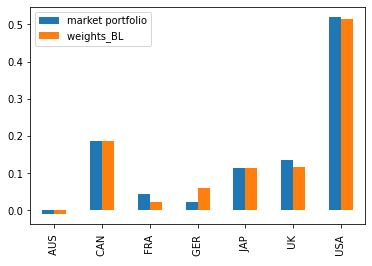
\includegraphics[width=0.5\textwidth]{BL better.png}
    \caption{Market portfolio weigths vs. optimal BL weights}
    \label{fig:BL better}
\end{figure}
From \cref{fig:BL better} presented above, it is evident that the portfolio weights suggested by the BL model exhibit improved interpretability. As we are more optimistic about Germany, its weight is higher, while the weights of the UK and France are lower. This allocation aligns with investor expectations and is more easily accepted compared to the MVO framework.

The weights of other countries remain equal to those in the market equilibrium state, unaffected by our subjective judgments, which echo back the idea behind the BL framework where the investor maintains the market portfolio if they don't have views. Such mechanics increase the lower bound of the return of the portfolio yields by the BL model and add to the robustness of the weights provided by the BL framework.

\textbf{Pros:}
\begin{enumerate}
\item Better interpretability comparing to the classical MVO framework.
\item More stable/robust comparing to the classical MVO.
\item It's relatively simple. The investor is now no longer obliged to specify views on all assets, but can specify views only if she holds one.
\end{enumerate}
\textbf{Cons:}
\begin{enumerate}
\item The BL model assumes that security returns are normally distributed, which is not realistic empirically speaking.
\item The assumption that investment views are linear portfolios of the securities excludes the use of nonlinear views that are pervasive in options strategies, such as tail-risk hedging overlays.
\item The prior distribution in the classical BL model is provided by the CAPM market equilibrium portfolio, where a number of factors, in addition to the market factor, are important for the derivation of prior returns.
\item The confidence of views, represented by $\tau$, and the risk-aversion coefficient, represented by $\delta$, are difficult to calibrate. We can only rely on rules of thumb for their determination.
\end{enumerate}

\subsection{Practical Considerations about the Black-Litterman Model}

\subsubsection{What Should the Magnitude of ${\tau}$ Be?}

Recall that
$$
\bm{\mu} \sim \mathcal{N}(\bm{\pi}, \tau \mathbf{\Sigma}) \quad \text { (market equilibrium) }
$$
The sample estimator
$$
\bm{\hat{\bm{\mu}}}=\frac{1}{T} \sum_{t=1}^{T} \bm{\bm{r}}_{i} \sim \mathcal{N}\left(\bm{\pi}, \frac{1}{T} \mathbf{\Sigma}\right)
$$
Therefore it is sensible that $\tau \propto \frac{1}{T}$.

\subsubsection{Calibrating the Confidence in the Views, $\mathbf{\Omega}$}

$$
\mathbf{P} \bm{\mu} \sim \mathcal{N}(\bm{q}, \mathbf{\Omega}) \quad \text { (investor's views) }
$$
In many cases we may not have a direct estimate of the confidence (variance) of a view, so we have to apply other tools to find it out. We have several ways to do this:
\begin{enumerate}
    \item Using the prior $\mathbf{\Omega}=\mathbf{P} \tau \mathbf{\Sigma} \mathbf{P}^{\top}$ or  $\mathbf{\Omega}=\operatorname{diag}\left(\mathbf{P} \tau \mathbf{\Sigma} \mathbf{P}^{\top}\right)$ .
    \item Using confidence intervals like we did in the example above.
    \begin{remark}
        Let us say that we believe there is a $95\%$ chance that the first view in \cref{subsubsec:investor's views} will happen. If we assume normality, we can interpret this as a $95\%$ confidence interval for the future return to be in the interval $[3\%-3.9\%, 3\%+3.9\%]$. From this confidence interval we calculate that the implied standard deviation ($\sigma_1$) is equal to about $2\%$. Therefore, we would set the Black-Litterman confidence equal to $(2\%)^2 = 0.04\%$.
    \end{remark}
    \item From backtesting the trading strategies (\bm{e}.g. long-short strategy) corresponding to the views.

    \begin{remark}We could estimate its historical variance through simulation with historical data. Of course, we cannot completely judge the performance of a strategy going forward from our backtests. Nevertheless, the back-test methodology allows us to obtain an estimate of the Black-Litterman view and confidence for a particular view/strategy.
    \end{remark}
    
    \item Factor models (cross-sectional or time-series).
    \begin{remark}
        APT models are especially useful as they provide a covariance matrix estimator that, unlike the sample covariance matrix, leads to stable, well-diversified optimal portfolios. This is provided when you have great risk factors, solid estimation techniques, and a big, well-constructed portfolio.
    \end{remark}
\end{enumerate}
\subsection{Connecting the Black-Litterman model with APT}
{\color{C6}\textbf{Intuition:} Our goal is to determine how our view, denoted as $\bm{q}$, influences the distribution of $\bm{r}$, specifically $\mathbb{E}[\bm{r}]$ and $\mathbb{V}[\bm{r}]$. To achieve this, we introduce a latent parameter, $\bm{\theta}$, as an intermediary. This parameter could represent $\mathbb{E}[\bm{r}]$ or the expected value of other factors related to $\bm{r}$. We first consider the prior of $\bm{\theta}$, then apply Bayesian techniques to update $\bm{\theta}$ and obtain the posterior $\bm{\theta}|\bm{q}$. Finally, we use this posterior of $\bm{\theta}$ to update the distribution of $\bm{r}$, employing $\bm{r}|\bm{\theta} \cdot \bm{\theta}|\bm{q}$.}

This is proposed by Petter Klom and Gordon Ritter(2017).
\subsubsection{Formulation}
{\color{C6}\textbf{Motivation:} Instead of analyzing the distribution of parameter $\bm{\theta}=\mu$, the expected return of $\bm{r}$ directly as in the classical Black-Litterman Framework, i.e.
\[
\bm{r} \xleftarrow[]{Bayesian}\bm{q},
\]we investigate the distribution of expected factor risk premia $\bm{\theta}=\EE[\bm{f}]$, then use the APT model to bridge the gap between $\bm{r}$ and $f$, i.e.
\[
\bm{r} \xleftarrow[\bm{r}|\bm{q}\quad \Longleftarrow \quad\bm{r}|\bm{\theta}\cdot \bm{\theta}|\bm{q}]{Bayesian}\bm{\theta}|\bm{q}\xleftarrow[\bm{\theta}|\bm{q}\quad \Longleftarrow \quad \bm{q}|\bm{\theta}\cdot \pi(\theta)]{Bayesian}\bm{q}.
\]}

\begin{definition}\label{def:Essential Ingredients of the BLB model}
    \textbf{(Essential Ingredients)} 
    \begin{enumerate}[label=(\alph*)]
        \item A parametric statistical model for asset returns $p(\bm{r} | \bm{\theta})$ with finite-dimensional parameter vector $\bm{\theta}$,
        \item A prior $\pi(\bm{\theta})$ on the parameter space,
        \item A likelihood function $f(\bm{q} | \bm{\theta})$ where $\bm{\theta}$ is any parameter vector appearing in a parametric statistical model for asset returns, and $\bm{q}$ is a vector supplied by portfolio managers or economists.
        \item Explicitly, the posterior predictive density of $\bm{r}$ is given by
$$
\begin{aligned}
& p(\bm{r} | \bm{q})=\int p(\bm{r} | \bm{\theta}) p(\bm{\theta} | \bm{q}) d \bm{\theta} \quad \text { where } \\
& p(\bm{\theta} | \bm{q})=\frac{f(\bm{q} | \bm{\theta}) \pi(\bm{\theta})}{\int f(\bm{q} | \bm{\theta}) \pi(\bm{\theta}) d \bm{\theta}}
\end{aligned}
$$
    \end{enumerate}
\end{definition} 
\begin{remark}\hfill
\begin{enumerate}
    \item  Items (a) and (b) simply state that we have a Bayesian statistical model, as defined in \cref{sec:Bayesian Statistical Model}, for asset returns.
    \item We are free to choose $\boldsymbol{\theta}$ as any vector of parameters appearing in a parametric statistical model for asset returns.
\end{enumerate}
   
\end{remark}

{\color{C6}\textbf{Step 0:} Introduce the APT model.}

From \cref{sec:APT in Matrix Form}, we know that the APT model states
$$
\bm{r}=\mathbf{X} \bm{f}+\bm{\varepsilon}, \quad \mathbb{E}[\bm{\varepsilon}]=0, \quad \mathbb{V}[\bm{\varepsilon}]=\mathbf{D}
$$
where 
\begin{itemize}
    \item $\bm{r} \in \mathbb{R}^{n}$ is an $n$-dimensional random vector containing the crosssection of \textbf{returns in excess of the risk-free rate} over some time interval $[t, t+1]$,
    \item $\mathbf{X} \in \mathbb{R}^{n\times k}$ is a (non-random) $n \times k$ matrix for factor loadings that is known before time $t$,
    \item $\bm{f} \in \mathbb{R}^{k}$ denotes a $k$-dimensional random vector process for latent factors which cannot be observed directly,
    \item $k \ll n$,
    \item $\bm{\varepsilon} \in \mathbb{R}^{n}$ is assumed to follow a mean-zero distribution with diagonal variance-covariance matrix given by $\mathbf{D}=diag\left(\sigma_1^2, \ldots, \sigma_n^2\right)$ with all $\sigma_i^2>0$.
\end{itemize}  

Also from \cref{prop:APT Useful Technique}, we know that if the $\bm{f}$-process is assumed to have finite first and second moments as 
$$
\mathbb{E}[\bm{f}]=\boldsymbol{\mu}_f, \text { and } ~\mathbb{V}[\bm{f}]=\mathbf{F}
$$
then 
\begin{align}
    \mathbb{E}[\bm{r}]=\mathbf{X} \boldsymbol{\mu}_f, \text{ and } \mathbb{V}[\bm{r}]=\mathbf{D}+\mathbf{X} \mathbf{F} \mathbf{X}^{\top}
\end{align}
where $\mathbf{X}^{\top}$ denotes the transpose of $\mathbf{X}$. 

{\color{C6}\textbf{Step 1:} Specify parameter $\bm{\theta}$.}

We are free to choose $\boldsymbol{\theta}$ as any vector of parameters appearing in a parametric statistical model for asset returns. Therefore, we use the APT model and choose 
\[
\boldsymbol{\theta}=\boldsymbol{\mu}_f, \text{ i.e. } \bm{f} \sim \mathcal{N}\left(\bm{\theta}, \mathbf{F}\right)
\]
which represents the $k$ parameters describing the factor risk premia.

For simplicity we treat $\mathbf{F}$ as a constant matrix, just as the original Black-Litterman model treats $\mathbf{\Sigma}$ as a constant matrix.


{\color{C6}\textbf{Step 2:} Choose the prior $\pi(\bm{\theta})$ for parameter $\bm{\theta}$.}

\begin{itemize}
    \item \textbf{Option 1:} Data-Driven Prior.

    In particular, we pick the historical mean and variance of the OLS estimates $\hat{\bm{f}}_t=\left(\mathbf{X}_t^{\top} \mathbf{X}_t\right)^{-1} \mathbf{X}_t^{\top} \boldsymbol{r}_{t+1}$ to be taken as the prior mean and prior variance. 

    \item \textbf{Option 2:} Benchmark-Optimal Prior.

    We choose prior such that $\pi(\boldsymbol{\theta}) \sim \mathcal{N}(\boldsymbol{\xi}, \boldsymbol{V})$ with $\boldsymbol{\xi} \in \mathbb{R}^k$ and symmetric positive definite matrix $\boldsymbol{V} \in \mathbb{R}^{k\times k}$. At this prior state, we have a prior distribution of $\bm{r}$ given by $p(\boldsymbol{r})=\int p(\boldsymbol{r} | \boldsymbol{\theta}) \pi(\boldsymbol{\theta}) d \boldsymbol{\theta}$ where $p(\boldsymbol{r} | \boldsymbol{\theta})$ is given by the APT model. Under this distribution $p(\boldsymbol{r})$, we have the corresponding $\mathbb{E}[\boldsymbol{r}]$ and $\VV[\boldsymbol{r}]$, which yields a optimal portfolio weights under a specified utility function given by the MVO framework, and we call this portfolio the benchmark portfolio $\bm{w}_B$, or the priori optimal portfolio.
\end{itemize}

{\color{C6}\textbf{Step 3:} Calculate the optimal portfolio $\bm{w}^*$, along with its mean and variance, at the prior state.}

Now, we treat $\pi(\boldsymbol{\theta}) \sim\mathcal{N}(\boldsymbol{\xi}, \boldsymbol{V})$ as if the expected return $\boldsymbol{\xi}$ and covariance $\boldsymbol{V}$ are known. Let's calculate the priori optimal portfolio/benchmark portfolio $\bm{w}_B$.  

\begin{solution}
The first step is to compute the a priori density of $\bm{r}$, $p(\boldsymbol{r})=\int p(\boldsymbol{r} | \boldsymbol{\theta}) \pi(\boldsymbol{\theta}) d \boldsymbol{\theta}$. 
Since $\pi(\boldsymbol{\theta})$ and $p(\boldsymbol{r} | \boldsymbol{\theta})$ are both Gaussian, this is another completion of squares.

For simplicity, we define the asset-level covariance in the APT model as 
\[
\mathbf{\Sigma}:=\mathbb{V}[\bm{r}]=\mathbf{D}+\mathbf{X} \mathbf{F} \mathbf{X}^{\top}
\]
Then, we have $\boldsymbol{r} \mid \boldsymbol{\theta} \sim \mathcal{N}\left(\mathbf{X} \boldsymbol{\theta}, \mathbf{\Sigma}\right)$, and 
\[
p(\boldsymbol{r} \mid \boldsymbol{\theta}) = \exp \left[-\frac{1}{2}(\boldsymbol{r}-\mathbf{X} \boldsymbol{\theta})^{\top} \mathbf{\Sigma}^{-1}(\boldsymbol{r}-\mathbf{X}\boldsymbol{\theta})\right],~ \pi(\boldsymbol{\theta}) = \exp \left[-\frac{1}{2}(\boldsymbol{\theta}-\boldsymbol{\xi})^{\top} \mathbf{V}^{-1}(\boldsymbol{\theta}-\boldsymbol{\xi})\right]
\]
Straightforward calculations then show:
$$
\begin{aligned}
p(\boldsymbol{r} \mid \boldsymbol{\theta}) \pi(\boldsymbol{\theta}) & =\exp \left[-\frac{1}{2}(\boldsymbol{r}-\mathbf{X} \boldsymbol{\theta})^{\top} \mathbf{\Sigma}^{-1}(\boldsymbol{r}-\mathbf{X}\boldsymbol{\theta})\right]\cdot \exp \left[-\frac{1}{2}(\boldsymbol{\theta}-\boldsymbol{\xi})^{\top} \mathbf{V}^{-1}(\boldsymbol{\theta}-\boldsymbol{\xi})\right] \\
& =\exp\left[-\frac{1}{2}\left((\boldsymbol{r}-\mathbf{X} \boldsymbol{\theta})^{\top} \mathbf{\Sigma}^{-1}(\boldsymbol{r}-\mathbf{X} \boldsymbol{\theta})+(\boldsymbol{\theta}-\boldsymbol{\xi})^{\top} \mathbf{V}^{-1}(\boldsymbol{\theta}-\boldsymbol{\xi})\right)\right] \\
& =\exp\left[-\frac{1}{2}\left(\boldsymbol{\theta}^{\top} \mathbf{H} \boldsymbol{\theta}-2 \boldsymbol{\eta}^{\top} \boldsymbol{\theta}+\boldsymbol{z}\right)\right]
\end{aligned}
$$
where the auxiliary variables
$$
\mathbf{H}=\boldsymbol{V}^{-1}+\mathbf{X}^{\top} \mathbf{\Sigma}^{-1} \mathbf{X}, \quad \boldsymbol{\eta}=\left(\boldsymbol{\xi}^{\top} \boldsymbol{V}^{-1}+\boldsymbol{r}^{\top} \mathbf{\Sigma}^{-1} \mathbf{X}\right)^{\top}, \quad \boldsymbol{z}=\boldsymbol{r}^{\top} \mathbf{\Sigma}^{-1} \boldsymbol{r}+\boldsymbol{\xi}^{\top} \boldsymbol{V}^{-1} \boldsymbol{\xi}
$$
Completing the square again,
$$
\boldsymbol{\theta}^{\top} \mathbf{H} \boldsymbol{\theta}-2 \eta^{\top} \boldsymbol{\theta}+\boldsymbol{z}=(\boldsymbol{\theta}-\bm{\nu})^{\top} \mathbf{H}(\boldsymbol{\theta}-\bm{\nu})-\bm{\nu}^{\top} \mathbf{H} \bm{\nu}+\boldsymbol{z}, \quad \bm{\nu}=\mathbf{H}^{-1} \eta
$$
Hence,
$$
\begin{aligned}
\int p(\boldsymbol{r} | \boldsymbol{\theta}) \pi(\boldsymbol{\theta}) d \boldsymbol{\theta}= &\int\exp\left[-\frac{1}{2}\left(\boldsymbol{\theta}^{\top} \mathbf{H} \boldsymbol{\theta}-2 \boldsymbol{\eta}^{\top} \boldsymbol{\theta}+\boldsymbol{z}\right)\right]d \boldsymbol{\theta}\\
= & \int\exp\left[-\frac{1}{2}\left((\boldsymbol{\theta}-\bm{\nu})^{\top} \mathbf{H}(\boldsymbol{\theta}-\bm{\nu})-\bm{\nu}^{\top} \mathbf{H} \bm{\nu}+\boldsymbol{z}\right)\right]d \boldsymbol{\theta}\\
= & \int\exp\left[-\frac{1}{2}(\boldsymbol{\theta}-\bm{\nu})^{\top} \mathbf{H}(\boldsymbol{\theta}-\bm{\nu})\right]d \boldsymbol{\theta}\cdot \exp \left[-\frac{1}{2}\left(\boldsymbol{z}-\boldsymbol{\nu}^{\top} \mathbf{H} \boldsymbol{\nu}\right)\right]\\
\text{Gaussian }\Longrightarrow= & \sqrt{(2 \pi)^k|\mathbf{H}^{-1}|} \exp \left[-\frac{1}{2}\left(\boldsymbol{z}-\boldsymbol{\nu}^{\top} \mathbf{H} \boldsymbol{\nu}\right)\right] \\
\bm{\nu}=\mathbf{H}^{-1} \eta\Longrightarrow= & \sqrt{\frac{(2 \pi)^k}{\operatorname{det} \mathbf{H}}} \exp \left[-\frac{1}{2}\left(\boldsymbol{z}-\boldsymbol{\eta}^{\top} \mathbf{H}^{-1} \boldsymbol{\eta}\right)\right] \\
= & \sqrt{\frac{(2 \pi)^k}{\operatorname{det} \mathbf{H}}} \exp \left[-\frac{1}{2}(\bm{r}^\top \mathbf{\Sigma}^{-1} \boldsymbol{r}+\boldsymbol{\xi}^{\top} \boldsymbol{V}^{-1} \boldsymbol{\xi}-\left(\boldsymbol{\xi}^{\top} \boldsymbol{V}^{-1}\right.\right. \\
& \left.\left.\left.+\boldsymbol{r}^{\top} \mathbf{\Sigma}^{-1} \mathbf{X}\right) \mathbf{H}^{-1}\left(\boldsymbol{V}^{-1} \boldsymbol{\xi}+\mathbf{X}^{\top} \mathbf{\Sigma}^{-1} \boldsymbol{r}\right)\right)\right]\\
= & \sqrt{\frac{(2 \pi)^k}{\operatorname{det} \mathbf{H}}} \exp \left[-\frac{1}{2}\left(\bm{r}^\top \left(\mathbf{\Sigma}^{-1} - \mathbf{\Sigma}^{-1} \mathbf{X} \mathbf{H}^{-1} \mathbf{X}^{\top} \mathbf{\Sigma}^{-1}\right) \boldsymbol{r}\right. \right.\\
& \left.\left.-2 \boldsymbol{\xi}^{\top}(\mathbf{H} \boldsymbol{V})^{-1} \mathbf{X}^{\top} \mathbf{\Sigma}^{-1} \boldsymbol{r}+\boldsymbol{\xi}^{\top} (\boldsymbol{V}^{-1}-(\boldsymbol{V} \mathbf{H} \boldsymbol{V})^{-1} ) \boldsymbol{\xi}\right)\right]
\end{aligned}
$$
Therefore, we have
\begin{align*}
\Longrightarrow -2\log p(\bm{r}) &= \bm{r}^\top \left(\mathbf{\Sigma}^{-1} - \mathbf{\Sigma}^{-1} \mathbf{X} \mathbf{H}^{-1} \mathbf{X}^{\top} \mathbf{\Sigma}^{-1}\right) \boldsymbol{r}-2 \boldsymbol{\xi}^{\top}(\mathbf{H} \boldsymbol{V})^{-1} \mathbf{X}^{\top} \mathbf{\Sigma}^{-1} \boldsymbol{r}\\
&\quad +(\text{ terms without }\boldsymbol{r})
\end{align*}
Note that $\int p(\boldsymbol{r} \mid \boldsymbol{\theta}) \pi(\boldsymbol{\theta}) \mathrm{d} \boldsymbol{\theta}$ is a Gaussian probability distribution for the random vector $\boldsymbol{r}$. Since matrices $\mathbf{V}$ and $\mathbf{D}$ are symmetric, matrices $\mathbf{\Sigma}$ and $\mathbf{H}$ are symmetric. Hence, we can set $\mathbf{M}=\left(\mathbf{\Sigma}^{-1} - \mathbf{\Sigma}^{-1} \mathbf{X} \mathbf{H}^{-1} \mathbf{X}^{\top} \mathbf{\Sigma}^{-1}\right)$ and $\bm{u}^\top=\boldsymbol{\xi}^{\top}(\mathbf{H} \boldsymbol{V})^{-1} \mathbf{X}^{\top} \mathbf{\Sigma}^{-1}$ in \cref{theo:A Useful Theorem}. Then, we have 
$$
\mathbb{V}_\pi[\boldsymbol{r}]=\mathbf{M}^{-1}=\left(\mathbf{\Sigma}^{-1} - \mathbf{\Sigma}^{-1} \mathbf{X} \mathbf{H}^{-1} \mathbf{X}^{\top} \mathbf{\Sigma}^{-1}\right)^{-1}
$$
and the mean is
$$
\begin{aligned}
\mathbb{E}_\pi[\boldsymbol{r}] =\mathbf{M}^{-1}\bm{u} & =\mathbb{V}_\pi[\boldsymbol{r}] \mathbf{\Sigma}^{-1} \mathbf{X} \mathbf{H}^{-1} \boldsymbol{V}^{-1} \xi \\
& =\left(\mathbf{\Sigma}^{-1} - \mathbf{\Sigma}^{-1} \mathbf{X} \mathbf{H}^{-1} \mathbf{X}^{\top} \mathbf{\Sigma}^{-1}\right)^{-1} \mathbf{\Sigma}^{-1} \mathbf{X} \mathbf{H}^{-1} \boldsymbol{V}^{-1} \boldsymbol{\xi}
\end{aligned}
$$
The a priori optimal portfolio under CARA utility is then
\begin{align}
   \bm{w}_B:=\bm{w}^*=\left(\lambda \mathbb{V}_\pi[\boldsymbol{r}]\right)^{-1} \mathbb{E}_\pi[\boldsymbol{r}]=\lambda^{-1} \mathbf{\Sigma}^{-1} \mathbf{X} \mathbf{H}^{-1} \boldsymbol{V}^{-1} \boldsymbol{\xi} \label{eq:priori optimal portfolio under CARA}
\end{align}
\end{solution}

\begin{remark}
    \hfill\begin{enumerate}
        \item At this prior state, we don't need $\bm{q}$. The view vector $\bm{q}$ is for us to update the distributions of $\bm{\theta}$ and $\bm{r}$; that is, it's for the posterior.
    \end{enumerate}
\end{remark}

{\color{C6}\textbf{Step 4:} Specify the view equation.}\label{seee:Specify the view equation }

A typical situation is when a quantitative portfolio manager has opinions on each factor risk premium, like the value premium or momentum premium. These opinions usually don't depend on their views on other factors. It's unusual, or almost impossible, for managers to have opinions on things like the total or difference of the value and momentum premiums, or more broadly on "portfolios of factors." So, we interpret the view equation as follows:
\[
\bm{\theta} = \bm{q} +\bm{\varepsilon}, \quad \bm{\varepsilon} \sim \mathcal{N}(\bm{0}, \mathbf{\Omega}), \quad \mathbf{\Omega}=\operatorname{diag}\left(\omega_1^2, \ldots, \omega_k^2\right)
\]
then, $\boldsymbol{q} | \boldsymbol{\theta} \sim \mathcal{N}(\bm{q}, \mathbf{\Omega})$ and the likelihood function is therefore
$$
f(\boldsymbol{q} | \boldsymbol{\theta})\propto\exp\left[-\frac{1}{2}(\bm{\theta}-\bm{q})^\top\mathbf{\Omega}^{-1}(\bm{\theta}-\bm{q})\right]=\prod_{i=1}^k \exp \left[-\frac{1}{2 \omega_i^2}\left(\theta_i-q_i\right)^2\right]
$$

{\color{C6}\textbf{Step 5:} Calculate the posterior distribution for $\bm{r}|\bm{q}$.}

\begin{enumerate}
    \item Calculate the posterior distribution for $\boldsymbol{\theta}|\bm{q}$, after the views are taken into account, which is given by
$$
p(\boldsymbol{\theta} \mid \boldsymbol{q})=\frac{f(\boldsymbol{q} \mid \boldsymbol{\theta}) \pi(\boldsymbol{\theta})}{\int f(\boldsymbol{q} \mid \boldsymbol{\theta}) \pi(\boldsymbol{\theta}) d \boldsymbol{\theta}}\propto f(\boldsymbol{q} \mid \boldsymbol{\theta}) \pi(\boldsymbol{\theta})
$$
\begin{solution}
    Since $\pi(\bm{\theta})$ is normal and the likelihood $f(\boldsymbol{q} | \boldsymbol{\theta})$ is also normal, the prior is a conjugate prior for the normal likelihood. Then, the posterior distribution $p(\boldsymbol{\theta} \mid \boldsymbol{q})$ is also normal.

    Using the relation above, we have
    \begin{align*}
        p(\boldsymbol{\theta} \mid \boldsymbol{q})
        &\propto f(\boldsymbol{q} \mid \boldsymbol{\theta}) \pi(\boldsymbol{\theta})\\
        &=\exp\left[-\frac{1}{2}(\bm{\theta}-\bm{q})^\top\mathbf{\Omega}^{-1}(\bm{\theta}-\bm{q})\right]\exp \left[-\frac{1}{2}(\boldsymbol{\theta}-\boldsymbol{\xi})^{\top} \mathbf{V}^{-1}(\boldsymbol{\theta}-\boldsymbol{\xi})\right]
    \end{align*}
    Therefore, we have
\begin{align*}
\Longrightarrow -2\log p(\boldsymbol{\theta} \mid \boldsymbol{q}) &= (\bm{\theta}-\bm{q})^\top\mathbf{\Omega}^{-1}(\bm{\theta}-\bm{q})+(\boldsymbol{\theta}-\boldsymbol{\xi})^{\top} \mathbf{V}^{-1}(\boldsymbol{\theta}-\boldsymbol{\xi})\\
&=\bm{\theta}^\top (\mathbf{\Omega}^{-1}+\mathbf{V}^{-1})\bm{\theta}-2(\bm{q}^\top \mathbf{\Omega}^{-1} + \boldsymbol{\xi}^\top \mathbf{V}^{-1})\bm{\theta}\\
&\quad +(\text{ terms without }\boldsymbol{\theta})
\end{align*}
 We set $\mathbf{M}=(\mathbf{\Omega}^{-1}+\mathbf{V}^{-1})$ and $\bm{u}^\top=(\bm{q}^\top \mathbf{\Omega}^{-1} + \boldsymbol{\xi}^\top \mathbf{V}^{-1})$ in \cref{theo:A Useful Theorem}. Then, we have 
$$
\mathbb{V}[\boldsymbol{\theta} \mid \boldsymbol{q}]=\mathbf{M}^{-1}=(\mathbf{\Omega}^{-1}+\mathbf{V}^{-1})^{-1}
$$
and the mean is
$$
\begin{aligned}
\mathbb{E}[\boldsymbol{\theta} \mid \boldsymbol{q}] =\mathbf{M}^{-1}\bm{u} & =\mathbb{V}[\boldsymbol{\theta} \mid \boldsymbol{q}] \left(\boldsymbol{V}^{-1} \boldsymbol{\xi}+\boldsymbol{\Omega}^{-1} \boldsymbol{q}\right) \\
& =\left(\boldsymbol{V}^{-1}+\boldsymbol{\Omega}^{-1}\right)^{-1}\left(\boldsymbol{V}^{-1} \boldsymbol{\xi}+\boldsymbol{\Omega}^{-1} \boldsymbol{q}\right)
\end{aligned}
$$
Therefore, the posterior must satisfy
\[
\boldsymbol{\theta} \mid \boldsymbol{q} \sim \mathcal{N}(\widetilde{\boldsymbol{\xi}}, \widetilde{\boldsymbol{V}})
\]
where $\widetilde{\boldsymbol{V}}=\left(\boldsymbol{V}^{-1}+\boldsymbol{\Omega}^{-1}\right)^{-1}, \quad \widetilde{\boldsymbol{\xi}}=\left(\boldsymbol{V}^{-1}+\boldsymbol{\Omega}^{-1}\right)^{-1}\left(\boldsymbol{V}^{-1} \boldsymbol{\xi}+\boldsymbol{\Omega}^{-1} \boldsymbol{q}\right)$
\end{solution}
\item Calculate the a posteriori distribution of asset returns (also called the posterior predictive density), given by
$$
p(\boldsymbol{r} \mid \boldsymbol{q})=\int p(\boldsymbol{r} \mid \boldsymbol{\theta}) p(\boldsymbol{\theta} \mid \boldsymbol{q}) d \boldsymbol{\theta}
$$
\begin{solution}
    For this one, we can view $p(\boldsymbol{\theta} \mid \boldsymbol{q})$ as the prior density for $\bm{\theta}$, then the situation here is the same as in {\color{C6}\textbf{Step 3}}. Hence, use the result in {\color{C6}\textbf{Step 3}} and make the substitution $\boldsymbol{\xi} \rightarrow \widetilde{\boldsymbol{\xi}}$ and $\boldsymbol{V} \rightarrow \widetilde{\boldsymbol{V}}$, we obtain
$$
\begin{aligned}
& \mathbb{V}[\boldsymbol{r} \mid \boldsymbol{q}]=\left(\boldsymbol{\Sigma}^{-1}-\boldsymbol{\Sigma}^{-1} \boldsymbol{X}\left(\widetilde{\boldsymbol{V}}^{-1}+\boldsymbol{X}^{\top} \boldsymbol{\Sigma}^{-1} \boldsymbol{X}\right)^{-1} \boldsymbol{X}^{\top} \boldsymbol{\Sigma}^{-1}\right)^{-1} \\
& \mathbb{E}[\boldsymbol{r} \mid \boldsymbol{q}]=\mathbb{V}[\boldsymbol{r} \mid \boldsymbol{q}] \boldsymbol{\Sigma}^{-1} \boldsymbol{X}\left(\widetilde{\boldsymbol{V}}^{-1}+\boldsymbol{X}^{\top} \boldsymbol{\Sigma}^{-1} \boldsymbol{X}\right)^{-1} \widetilde{\boldsymbol{V}}^{-1} \widetilde{\boldsymbol{\xi}}
\end{aligned}
$$
\end{solution}
\end{enumerate}

{\color{C6}\textbf{Step 6:} Calculate the mean-variance optimal portfolio.}

\begin{solution}
\begin{align*}
\bm{w}^*
&=\lambda^{-1} \mathbb{V}[\boldsymbol{r} \mid \boldsymbol{q}]^{-1} \mathbb{E}[\boldsymbol{r} \mid \boldsymbol{q}]\\
&=\lambda^{-1}\boldsymbol{\Sigma}^{-1} \boldsymbol{X}\left(\widetilde{\boldsymbol{V}}^{-1}+\boldsymbol{X}^{\top} \boldsymbol{\Sigma}^{-1} \boldsymbol{X}\right)^{-1} \widetilde{\boldsymbol{V}}^{-1} \widetilde{\boldsymbol{\xi}}
\end{align*}
\end{solution}

\newpage
\section{Meucci's framework}
In the realm of financial modelling and investment strategy, Meucci's framework stands out as an exceptional approach. Its superiority can be attributed to several compelling factors. Firstly, it significantly enhances our understanding of market dynamics and allocation strategies by providing profound insights into market invariants. Secondly, the framework is exhaustive, seamlessly integrating all stages of the investment process, from inception to culmination. Finally, the hallmark of Meucci's framework is its extraordinary versatility, reminiscent of a set of LEGO bricks. It offers the flexibility to effortlessly modify or substitute estimation methods or allocation techniques as required. This adaptability grants an unparalleled level of freedom in its application, further emphasizing the unique advantages of Meucci's framework.
\subsection{Investor's Profile}
{\color{C6}\textbf{Idea:} The investor's profile consists of $3$ major parts to describe the investor's intention.}
\begin{enumerate}
\item \textbf{Target Market:} The market the investor wants to invest in. For an option trader, the market is the option market; for a retiree, the market is a set of mutual funds.
\item \textbf{Investment Horizon $\tau$:} How long the action of investing is going to last, e.g., A day-trader aims at cashing profits within a few hours from the investment decision. A retiree has an investment horizon of the order of a few years.
\item \textbf{Investor's Objective:} The quantity $\Psi_{\bm{\alpha}}$ that an investor wants to maximize.
\[
\Psi_{\bm{\alpha}} \equiv \bm{\alpha}^{\top}\mathbf{M}, \quad \mathbf{M} = \bm{a} +\mathbf{B}\mathbf{P}_{T+\tau}
\]
where $\bm{a}$ is a suitable conformable vector and $\mathbf{B}$ is a suitable conformable invertible matrix.

    \textbf{Context:} Suppose the vector of prices of $n$ securities at a generic time $t\in\mathbb{R}$ is $\mathbf{P}_{t}\in\mathbb{R}^{n}$ (a vector of random variables), the vector of portfolio weights is $\bm{\alpha}\in\mathbb{R}^{n}$, the investment horizon is $\tau\in\mathbb{R}$, and the investor makes the investment decision at time $T\in\mathbb{R}$. Then, the investor's current wealth is $W_T(\bm{\alpha})=\bm{\alpha}^\top \mathbf{p}_T$ where we use lower case to emphasize the fact that at the current time $T$, the price for securities is known. His/Her wealth at the end of his investment horizon $T+\tau$ is $W_{T+\tau}(\bm{\alpha})=\bm{\alpha}^\top \mathbf{P}_{T+\tau}$. Then, the investor might have the following objectives $\Psi_{\bm{\alpha}}$:
    \begin{itemize}
        \item \textbf{Absolute wealth/Final wealth (For average human/retail investor):}
        
The total amount of money you have at the end of your investment horizon.
$$
\Psi_{\bm{\alpha}} \equiv W_{T+\tau}(\bm{\alpha})=\bm{\alpha}^{\top} \mathbf{P}_{T+\tau}=\bm{\alpha}^{\top}\mathbf{M}_{\text{absolute wealth}}
$$
where $\mathbf{M}_{\text{absolute wealth}}=\mathbf{P}_{T+\tau}, \bm{a}=\bm{0}, \mathbf{B}=\mathbf{I}_n$.
\item \textbf{Relative wealth (For portfolio manager):}
The total excess amount of money you have at the end of your investment horizon with respect to a benchmark.
\begin{align*}
\Psi_{\bm{\alpha}} &\equiv W_{T}(\bm{\alpha})\left(\frac{W_{T+\tau}(\bm{\alpha})}{W_{T}(\bm{\alpha})}-\frac{W_{T+\tau}(\bm{\alpha_{\text{benchmark}}})}{W_{T}(\bm{\alpha_{\text{benchmark}}})}\right)\\&=\bm{\alpha}^\top\left(\mathbf{I}_n-\frac{\mathbf{p}_T\bm{\alpha}_{\text{benchmark}}^\top}{\bm{\alpha}_{\text{benchmark}}^\top \mathbf{p}_T}\right)\mathbf{P}_{T+\tau}\\
&\bm{\alpha}^\top\mathbf{M}_{\text{realative wealth}}
\end{align*}
where $\mathbf{M}_{\text{realative wealth}}=\left(\mathbf{I}_n-\frac{\mathbf{p}_T\bm{\alpha}_{\text{benchmark}}^\top}{\bm{\alpha}_{\text{benchmark}}^\top \mathbf{p}_T}\right)\mathbf{P}_{T+\tau}, \bm{a}=\bm{0}, \mathbf{B}=\left(\mathbf{I}_n-\frac{\mathbf{p}_T\bm{\alpha}_{\text{benchmark}}^\top}{\bm{\alpha}_{\text{benchmark}}^\top \mathbf{p}_T}\right)$.
\item \textbf{Net profits (For traders):}
The profit you have at the end of your investment.
$$
\Psi_{\bm{\alpha}} \equiv W_{T+\tau}(\bm{\alpha})-w_T(\bm{\alpha})=\bm{\alpha}^{\top}\left(\mathbf{P}_{T+\tau}-\mathbf{p}_T\right) = \bm{\alpha}^{\top}\mathbf{M}_{\text{net profit}}
$$
where $\mathbf{M}_{\text{net profit}}=\left(\mathbf{P}_{T+\tau}-\mathbf{p}_T\right), \bm{a}=-\mathbf{p}_T, \mathbf{B}=\mathbf{I}_n$.
    \end{itemize}
\item \textbf{Investment constraints:}
For instance, consider budget constraints: these reflect the amount of money the investor is willing to invest at the time they make their investment decisions. Normally, this also takes into account transaction costs.
 
\end{enumerate}
\begin{remark}
    We see that the objective function $\Psi_{\bm{\alpha}}$ is 
    \begin{itemize}
        \item homogeneous of first degree:
        $$
\Psi_{\lambda \alpha}=\lambda \Psi_\alpha 
$$
\item additive:
$$
\Psi_{\alpha+\beta}=\Psi_\alpha+\Psi_\beta.$$
    \end{itemize}
These properties allow building and \textbf{comparing} objectives that refer to complex portfolios of securities.
\end{remark}


%%%%%%%%%%%%%%%%%%%%%%%%%%%%%%%%%%%
\subsection{Modeling the Market}
{\color{C6}\textbf{Idea:} The idea from Meucci's book, Risk and Asset Allocation, is that we first find an invariant $X_{t,\tau}$ for the target market, and then model this invariant using some statistical techniques on some small interval $\tilde{\tau}$ which is typically smaller than the investment horizon $\tau$. Next, we project the estimated invariant $X_{t,\tilde{\tau}}$ on to $X_{T+\tau}$ to find the estimated invariant for the investment horizon. Then we project the estimated invariant for the investment horizon to prices of the securities $\mathbf{P}_{T+\tau}$ via some mapping. Finally, we can do whatever we want with the estimated prices.}

\subsubsection{Find Market's Invariants}
To ascertain this, we fix an estimation interval $\tilde{\tau}$(e.g. one week) and a starting point $\tilde{t}$ (e.g. five years ago) and we consider the set of stock prices at the equally spaced estimation times 
$$
P_t, \quad t \in \mathcal{D}_{\tilde{t}, \widetilde{\tau}}, \quad \mathcal{D}_{\tilde{t}, \widetilde{\tau}}=\{\tilde{t}, \widetilde{t}+\widetilde{\tau}, \ldots, T\}
$$
Each of these random variables becomes available at the respective time $t$. 

We want the market invariant $X_{t,\tilde{\tau}}$ to have the following desired properties:
\begin{itemize}
    \item $X_{t,\tilde{\tau}}$'s are \textbf{identically distributed.}

    We apply the \textbf{Split Test} to examine this property where you split the time series $X_{t,\tilde{\tau}}, t\in \mathcal{D}_{\tilde{t}, \widetilde{\tau}}$ into two series:
$$
\begin{aligned}
& X_{t,\tilde{\tau}}, \quad t=\widetilde{t}, \ldots, \widetilde{t}+\left[\frac{T-\widetilde{t}}{2 \widetilde{\tau}}\right] \widetilde{\tau} \\
& X_{t,\tilde{\tau}}, \quad t=\left(\left[\frac{T-\widetilde{t}}{2 \widetilde{\tau}}\right]+1\right) \widetilde{\tau}, \ldots, T,
\end{aligned}
$$
where $[\cdot]$ denotes the floor operator. Then we compare the respective histograms. If $X_{t,\tilde{\tau}}$ is an invariant, in particular all the terms in the series are identically distributed: therefore the two histograms should look very similar to each other.
\item $X_{t,\tilde{\tau}}$'s are \textbf{independent of each other.}

We apply the \textbf{Lag Plot Test} to examine this property where you plot $x_t$ versus $x_{t-\tilde{\tau}}, \quad t=\tilde{t}+\widetilde{\tau}, \ldots, T$.

If $X_t$ is an invariant, in particular all the terms in the series are independent of each other: therefore the scatter plot must be symmetrical with respect to the reference axes. Furthermore, since all the terms are identically distributed, the scatter plot must resemble a circular cloud.
\item $X_{t,\tilde{\tau}}$ is \textbf{time homogeneous.}i.e. It doesn't depend on a well chosen starting time $\tilde{t}$.
\item $X_{t,\tilde{\tau}}$ is \textbf{additive.} Specifically, it would be better if it is in a form of differences.
\end{itemize}

\begin{remark}
    In Meucci's book, he purposed to use Elliptical distribution which is a generalization of the normal distribution, to model the distribution of the market invariant. This is too much of an overkill, we just stick to model the distribution of the market invariant by multivariate normal distribution.
\end{remark}
\begin{proposition}\label{prop:Invariants for specific markets}
    \textbf{(Invariants for Specific Markets)}
    \begin{enumerate}
        \item \textbf{Equities, commodities, exchange rates:} $X_{t,\tilde{\tau}}$ is compounded returns where 
the compounded return at time $t$ for a horizon $\tau$ is defined as follows:
$$
C_{t, \tilde{\tau}} \equiv \ln \left(\frac{P_t}{P_{t-\tilde{\tau}}}\right), t\in \mathcal{D}_{\tilde{t}, \widetilde{\tau}}
$$
\item \textbf{Fixed-income market:} $X_{t,\tilde{\tau}}$ is changes in yield to maturity $$
X_{t, \widetilde{\tau}}^{(v)} \equiv Y_t^{(v)}-Y_{t-\widetilde{\tau}}^{(v)}
$$
where the yield to maturity of a zero-coupon bond that expires at time $T+v$ at a generic time $t$ is defined as follows:
$$
Y_t^{(v)} \equiv-\frac{1}{v} \ln \left(Z_t^{(t+v)}\right)
$$, $Z_t^{(E)}$ is a zero-coupon bond that a certain amount of money  is turned in at the generic time $t$ and a (larger) determined amount is received back at a later, specified maturity date $E$. Since the amount to be received is determined, we can normalize it as follows without loss of generality:
$$
Z_E^{(E)} \equiv 1.
$$
\item \textbf{Derivatives:} $X_{t,\tilde{\tau}}$ is changes in at-the-money-forward (ATMF) implied percentage volatility with generic fixed rolling expiry $v$:
$$
X_{t, \widetilde{\tau}}^{(v)} \equiv \sigma_t^{\left(K_t, t+v\right)}-\sigma_{t-\tilde{\tau}}^{\left(K_{t-\tilde{\tau}}, t-\tilde{\tau}+v\right)}, \quad t \in \mathcal{D}_{\tilde{t}, \tilde{\tau}} .
$$
Each of these random variables becomes available at the respective time $t$.
    \end{enumerate}
Then, we can compress alll of the market invariants in one single vector, and denote it by $\mathbf{X}_{t, \tilde{\tau}}\in \mathbb{R}^d$.
\end{proposition}

\subsubsection{Model the distribution of the market invariants}
\textbf{Context:} Suppose we have  our market invariant $\mathbf{X}_{t, \tilde{\tau}}\in \mathbb{R}^d, t\in \mathcal{D}_{\tilde{t}, \widetilde{\tau}}=\{\tilde{t}, \widetilde{t}+\widetilde{\tau}, \ldots, T\}$, and, by choice, they are i.i.d., time homogeneous and additive. Now, we want to estimate it. WLOG, we can reduce our notation for invariants to time series vectors $$\mathbf{x}_{t}\in \mathbb{R}^d, t\in \{1,2,3,\ldots, N\}$$ via a linear mapping on the original $t$ where $N$ is an integer. 

\subsubsection{Non-parametric estimators}
These estimators are based on the law of large numbers. Therefore, they perform well when the number of empirical observations in the time series of the market invariants is large.
\begin{proposition}
    \textbf{(Plug-in Estimators)}\begin{itemize}
    \item \textbf{Sample Mean:} $\widehat{\mathrm{E}}\left[\mathbf{x}\right] =\frac{1}{N} \sum_{t=1}^N \mathbf{x}_t$.
    \item \textbf{Sample Covariance:} $\widehat{\operatorname{Cov}}\left[\mathbf{x}\right]=\frac{1}{N} \sum_{t=1}^N\left(\mathbf{x}_t-\widehat{\mathrm{E}}\left[\mathbf{x}\right]\right)\left(\mathbf{x}_t-\widehat{\mathrm{E}}\left[\mathbf{x}\right]\right)^{\top}$
\end{itemize}
\end{proposition}
\begin{remark}
    Not good at handling outliers.
\end{remark}

\begin{proposition}
    \textbf{(Kernel Density Estimators)} The basic idea behind KDE is to smooth out the data by replacing each data point with a small
kernel, or ``bump,” centered at that point. The kernels are typically Gaussian (bell-shaped) functions,
but other shapes can be used as well. The kernels for different data points are then added together
to create a continuous estimate of the probability density function $f_{\mathbf{x}}$. Suppose the bandwidth $\mathbf{H}=diag(h^2, \ldots, h^2)\in \mathbb{R}^{d\times d}$ and the kernel function is $$K(\mathbf{x})= \frac{1}{(2 \pi)^{\frac{d}{2}}} e^{-\frac{1}{2 }\mathbf{x}^{\top}\mathbf{x}}\sim \mathcal{N}(\bm{0}, \mathbf{I}), \quad K_{\mathbf{H}}(\mathbf{x})=|\mathbf{H}|^{-1 / 2} K\left(\mathbf{H}^{-1 / 2} \mathbf{x}\right)$$
Then, the kernel density estimate is 
\begin{align*}
\hat{f}_{\mathbf{x}} \mapsto \hat{f}_{\mathbf{x} ; \mathbf{H}} &\equiv  
\frac{1}{N} \sum_{t=1}^N K_{\mathbf{H}}\left( \mathbf{x}-\mathbf{x}_t\right)\\
&=\frac{1}{N} \sum_{t=1}^N \frac{1}{(2 \pi)^{\frac{d}{2}} |\mathbf{H}|^{1 / 2} } e^{-\frac{1}{2 }\left(\mathbf{H}^{-1 / 2} (\mathbf{x}-\mathbf{x}_t)\right)^{\top}\left(\mathbf{H}^{-1 / 2}(\mathbf{x}-\mathbf{x}_t)\right)}\\
&= \frac{1}{N} \sum_{t=1}^N \frac{1}{(2 \pi)^{\frac{d}{2}} h^d} e^{-\frac{1}{2 h^2}\left(\mathbf{x}-\mathbf{x}_t\right)^{\top}\left(\mathbf{x}-\mathbf{x}_t\right)}    
\end{align*}
The outcome of this operation is a smoother empirical probability density function such as the one sketched in \cref{fig:Synthetic_data_2D_KDE} for $d=2$.
\begin{figure}[!htp]
    \centering
    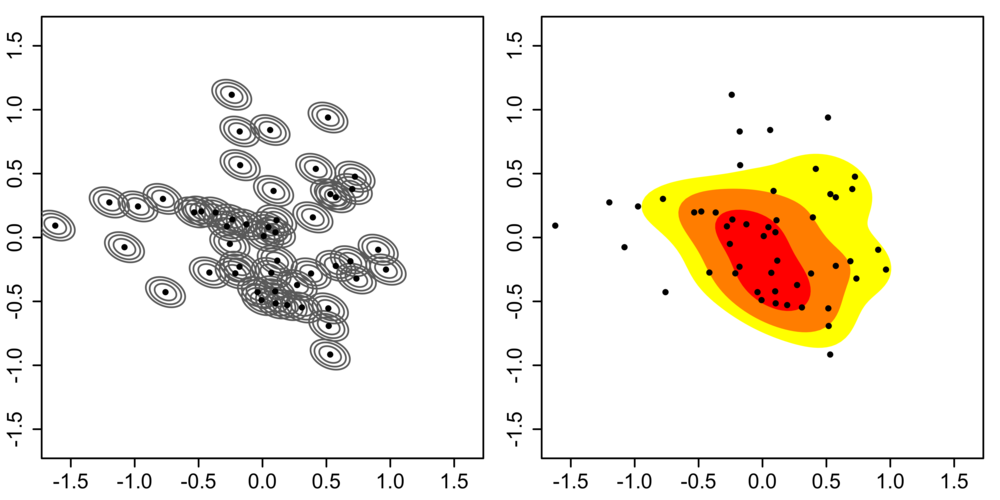
\includegraphics[width=0.5\textwidth]{Synthetic_data_2D_KDE.png}
    \caption{Construction of 2D kernel density estimate. Left. Individual kernels. Right. Kernel density estimate.}
    \label{fig:Synthetic_data_2D_KDE}
\end{figure}
\end{proposition}
\begin{remark}
        \item The bandwidth of the kernel must be chosen according to the following trade-off. A narrow bandwidth overfit, so the estimator produced is not robust; a wide bandwidth underfits, so the estimator produced gives rise to loss of information.
\end{remark}

\subsubsection{maximum likelihood estimators} MLE are built in such a way that the past observations of the market invariants, $\mathbf{x}_{t}\in \mathbb{R}^d, t\in \{1,2,3,\ldots, N\}$, become the most likely outcomes of the estimated parametric distribution. 

We assume the probability density function of the market invariant $\mathbf{x}_i$ (i.i.d.) to be $f_{\boldsymbol{\theta}}$, where $\boldsymbol{\theta}$ is an $S$-dimensional parameter that fully determines the distribution of $\mathbf{x}_i$ and that ranges in a given set $\Theta$.

Then, we want to maximize the likelihood function $f_{\boldsymbol{\theta}}\left(\mathbf{x}_1\right) \cdots f_{\boldsymbol{\theta}}\left(\mathbf{x}_T\right) $ of the time series, or we can maximize the log-likelihood function $\sum_{t=1}^T \ln f_{\boldsymbol{\theta}}\left(\mathbf{x}_t\right)$. Therefore the maximum likelihood estimator (MLE) of the parameters $\boldsymbol{\theta}$ is defined as follows:
$$
\widehat{\boldsymbol{\theta}}_{MLE} \equiv \underset{\boldsymbol{\theta} \in \boldsymbol{\Theta}}{\operatorname{argmax}} 
\prod_{t=1}^N  f_{\boldsymbol{\theta}}\left(\mathbf{x}_t\right) =\underset{\boldsymbol{\theta} \in \boldsymbol{\Theta}}{\operatorname{argmax}} \sum_{t=1}^N \ln f_{\boldsymbol{\theta}}\left(\mathbf{x}_t\right).
$$
\begin{property}
    \textbf{(Properties of MLE)} \begin{enumerate}[label=(\alph*)]
        \item  invariance property the MLE of a function of the parameters is that function applied to the MLE of the parameters:
$$
\widehat{g(\boldsymbol{\theta})}_{MLE}=g(\widehat{\boldsymbol{\theta}}_{MLE}).
$$
\item the following relation holds in approximation
$$
\widehat{\boldsymbol{\theta}}_{MLE} \sim \mathrm{N}\left(\boldsymbol{\theta}, \frac{\boldsymbol{\Gamma}}{T}\right) .
$$
 the approximation becomes exact as $T$ tends to infinity
 
In this expression $\Gamma$ is a symmetric and positive matrix called the Fisher information matrix:
$$
\boldsymbol{\Gamma} \equiv \operatorname{Cov}\left\{\frac{\partial \ln \left(f_{\boldsymbol{\theta}}(\mathbf{X})\right)}{\partial \boldsymbol{\theta}}\right\},
$$
\item The Cramer-Rao lower bound theorem states that the inefficiency of the maximum likelihood estimator, is the smallest possible achievable with an unbiased estimator.
    \end{enumerate} 
\end{property}

\begin{remark}
    When the number of observations is not very large. as it turns out, the main driver of the performance of the maximum likelihood estimators is the overall level of correlation among the market invariants, as summarized by the condition number.
\end{remark}

\subsubsection{Shrinkage Estimators}{\color{C6}When the number of observations is so small, it's time to use the shrinkage estimators.}

Suppose we have the sample mean and the sample covariance matrix:
$$
\widehat{\mathbf{m}} \equiv \frac{1}{T} \sum_{t=1}^T \mathbf{c}_{t, \tilde{\tau}}, \quad \widehat{\mathbf{S}} \equiv \frac{1}{T} \sum_{t=1}^T\left(\mathbf{c}_{t, \tilde{\tau}}-\widehat{\mathbf{m}}\right)\left(\mathbf{c}_{t, \tilde{\tau}}-\widehat{\mathbf{m}}\right)^{\top} .
$$
 We then shrink the covariance matrix toward a spherical estimator:
$$
\widehat{\mathbf{\Sigma}} \equiv(1-\epsilon) \widehat{\mathbf{S}}+\frac{\epsilon}{N} \sum_{n=1}^N \widehat{S}_{n n} \mathbf{I}_N
$$
where from  the shrinkage weight reads:
$$
\epsilon \equiv \frac{1}{T} \frac{\frac{1}{T} \sum_{t=1}^T \operatorname{tr}\left\{\left(\mathbf{c}_{t, \tilde{\tau}} \mathbf{c}_{t, \tilde{\tau}}^{\top}-\widehat{\mathbf{S}}\right)^2\right\}}{\operatorname{tr}\left\{\left(\widehat{\mathbf{S}}-\frac{1}{N} \sum_{n=1}^N \widehat{S}_{n n} \mathbf{I}_N\right)^2\right\}}
$$
Finally, we shrink the sample mean towards a target vector:
$$
\widehat{\boldsymbol{\mu}} \equiv(1-\gamma) \widehat{\mathbf{m}}+\gamma \mathbf{b}
$$
In this expression the shrinkage target follows from:
$$
\mathbf{b} \equiv \frac{\mathbf{1}^{\top} \widehat{\mathbf{\Sigma}}^{-1} \widehat{\mathbf{m}}}{\mathbf{1}^{\top} \widehat{\mathbf{\Sigma}}^{-1} \mathbf{1}} \mathbf{1}, \quad \gamma \equiv \frac{1}{T} \frac{\sum_{n=1}^N \widehat{\Sigma}_{n n}-2 \lambda_1}{(\widehat{\mathbf{m}}-\mathbf{b})^{\top}(\widehat{\mathbf{m}}-\mathbf{b})}
$$
where $\lambda_1$ is the highest eigenvalue of $\widehat{\Sigma}$.
% \subsubsection{robust estimation}

\subsubsection{Some practical tips}There are times we need to conduct special treatment to improve the estimation of the distribution of market invariants in specific situations.
\begin{enumerate}
    \item \textbf{Outliers:} We address outlier detection using high breakdown estimators, such as the minimum volume ellipsoid and the minimum covariance determinant.
    \item \textbf{Missing Data:} We handle missing data with the help of the EM algorithm.
    \item \textbf{Adjusting for economical understandings:} We use weighted estimation techniques like exponential smoothing, which takes into account the greater reliability of more recent data compared to older data.
\end{enumerate}




\subsection{Project the estimated invariants to the investment horizon}
{\color{C6}\textbf{Idea:} Basically, we want to find the distribution of $\boldsymbol{X}_{T+\tau, t}$ which is determined by $\phi_{\boldsymbol{X}_{T+\tau, t}}$ using the distribution of $\boldsymbol{X}_{T+\tilde{\tau}, \tilde{t}}$ which is determined by $
\phi_{\boldsymbol{X}_{T+\tilde{\tau}, \tilde{t}}}
$. 
\[
\boldsymbol{X}_{T+\tilde{\tau}, \tilde{t}} \mapsto \boldsymbol{X}_{T+\tau, t}
\]
With our fine choice of invariants, this is actually very easy to accomplish.}

Since all of our invariants are specifically chosen to be in the form of differences, they are additive, i.e. they satisfy the following relation:
$$
\mathbf{X}_{T+\tau, \tau}=\mathbf{X}_{T+\tau, \tilde{\tau}}+\mathbf{X}_{T+\tau-\tilde{\tau}, \tilde{\tau}}+\cdots+\mathbf{X}_{T+\tilde{\tau}, \tilde{\tau}} .
$$
Also, since the terms in the right-hand side of the equation above are invariants relative to non-overlapping time intervals, they are , by choice, independent and identically distributed random variables. Therefore, we must have
$$
\phi_{\mathbf{X}_{T+\tau, \tau}}=\left(\phi_{\mathbf{X}_{t, \tilde{\tau}}}\right)^{\frac{\tau}{\tau}}\Longleftrightarrow 
\mathbf{X}_{T+\tau, \tau} \sim \mathcal{N}\left(\frac{\tau}{\widetilde{\tau}} \widehat{\boldsymbol{\mu}}, \frac{\tau}{\widetilde{\tau}} \widehat{\boldsymbol{\Sigma}}\right) 
$$


\begin{remark}
    We conclude by pointing out that the simplicity of the projection formula hides the dangers of \textbf{estimation risk}. 
\end{remark}
\subsection{Map invariants to Prices}
Since we are dealing with raw securities, the pricing function has the following simple form:
$$
P_{T+\tau}=P_T e^X=e^{\mathbf{Y}}
$$
where the ancillary variable $\mathbf{Y}$ is an affine transformation of the market invariants:
$$
\mathbf{Y} \equiv \gamma+\operatorname{diag}(\varepsilon) \mathbf{X}
$$
where 
$\gamma_n \equiv\ln \left(P_T\right)$ and$\varepsilon_n \equiv1$.


\subsection{Evaluating Allocation}
Suppose we have an efficient frontier computed by the MVO framework. The question then becomes, how should we select the optimal allocation from all the options available on the efficient frontier? To aid decision-making, Meucci proposed a metric known as the "index of satisfaction." Generally, we use \textbf{Certainty-Equivalent} as satisfaction index:

\textbf{Certainty-Equivalent:} Here, we select a utility function and its associated risk-aversion coefficient. Assume we have an objective $\Psi_\alpha$. Then, we have
$$
\boldsymbol{\alpha}^* =\max_{\boldsymbol{\alpha}}\mathrm{CE}(\boldsymbol{\alpha}) \equiv \max_{\boldsymbol{\alpha}}u^{-1}\left(\mathrm{E}\left\{u\left(\boldsymbol{\alpha}^{\prime} \mathbf{M}\right)\right\}\right)
$$


\subsection{Mean-Variance Optimization}
{\color{C6}\textbf{Motivation:} The mean-variance framework can be viewed as an approximation of the more general framework, which involves the general index of satisfaction. This broader approach imposes significant computational challenges, making the mean-variance framework a more practical alternative.}


The investor's index of satisfaction is a functional of the distribution of the investor's objective. Since the distribution of the investor's objective is in general uniquely determined by its moments, the index of satisfaction can be re-written as a function defined on the infinite-dimensional space of the moments of the distribution of the objective:
$$
\mathcal{S}(\boldsymbol{\alpha}) \equiv \mathcal{H}\left(\mathrm{E}\left\{\Psi_\alpha\right\}, \mathrm{CM}_2\left\{\Psi_\alpha\right\}, \mathrm{CM}_3\left\{\Psi_\alpha\right\}, \ldots\right)\approx \tilde{\mathcal{H}}\left(\mathrm{E}\left\{\Psi_\alpha\right\}, \operatorname{Var}\left\{\Psi_\alpha\right\}\right) .
$$
for a suitable bivariate function $\tilde{\mathcal{H}}$, and $\mathrm{CM}_k$ denotes as in the central moment of order $k$ of a univariate distribution, $\mathrm{CM}_k\{\Psi\} \equiv \mathrm{E}\left\{(\Psi-\mathrm{E}\{\Psi\})^k\right\}$.

Then, we first solve 
$$
\boldsymbol{\alpha}(v) \equiv \underset{\substack{\alpha \in \mathcal{C} \\ \operatorname{Var}\left\{\Psi_\alpha\right\}=v}}{\operatorname{argmax}} \mathrm{E}\left\{\Psi_\alpha\right\}
$$
where $v \geq 0$ to get the efficient frontier. Then find the optimal allocation following the one-dimensional search:
$$
\boldsymbol{\alpha}^* \equiv \boldsymbol{\alpha}\left(v^*\right) \equiv \underset{v \geq 0}{\operatorname{argmax}} \mathcal{S}(\boldsymbol{\alpha}(v)).
$$


\begin{remark}
    I find Meucci's framework to be superior for several compelling reasons.
    \begin{enumerate}
        \item The insights it provides regarding market invariants enhance our comprehension of the market dynamics and allocation strategies.
        \item The framework is comprehensive, encompassing every step of the investment process from inception to culmination.
        \item Meucci's framework is exceptionally versatile. This flexibility is akin to a set of LEGO bricks, allowing for easy alterations and substitutions in estimation methods or allocation techniques as desired. This adaptability provides unparalleled freedom in its application.
    \end{enumerate}


\end{remark}





\newpage
\section{Empirical Example}
Now, let's delve into an empirical example. In this case, we use Meucci's framework as the foundation, and compare the performance of the MVO framework in various scenarios, as well as the effectiveness of the Black-Litterman APT model. Our findings suggest that to achieve a better PnL, improving the estimation of critical variables is paramount. By "better", I don't just mean statistically superior, but also more economically logical. Additionally, we demonstrated that the Black-Litterman-APT model is not the holy grain. It is only as efficient as its inputs.

\subsection{Investment Profile}
We denote as $\mathbf{P}_t$ the prices at the generic time $t$ of one share of the assets. Now, we initialize the necessary ingradients for our investment.

\begin{itemize}
    \item We assume investor's initial wealth is a given amount of cash $W=1000\$$.
    \item We assume that the investor chooses a set of $N \equiv 7$ stocks and that the investor plans to re-invest any dividends.
    \item We assume that the investment horizon is $\tau=3$ weeks.
    \item We assume that the investor's objective is final wealth:
$$
\Psi_\alpha \equiv \boldsymbol{\alpha}^{\top} \mathbf{P}_{T+\tau}
$$
where $T$ denotes the time investor makes his/her investment decision.
    \item We assume the investor cares about the certainty-equivalent of his expected utility  where his utility function is of the power type. 
    \[
    u(x) = x^{\frac{\gamma-1}{\gamma}}
    \]Therefore the investor's satisfaction reads:
$$
\mathcal{S}(\boldsymbol{\alpha}) =CE\equiv\left(\mathbb{E}\left\{\Psi_\alpha^{\frac{\gamma-1}{\gamma}}\right\}\right)^{\frac{\gamma}{\gamma-1}}
$$
We pick $\gamma =-9$ for the risk aversion parameter of the power utility functions.
\end{itemize}

\begin{remark}
    \hfill
    \begin{enumerate}
        \item Notice that the power utility function is defined only for positive values of the investor's objective. This is consistent with the fact that prices are positive and that the investor can only hold long positions in the stocks.
    \end{enumerate}
\end{remark} 

\subsection{Modeling the Market}
\begin{itemize}
    \item \textbf{Market Data:}
    \begin{itemize}
    \item The time-series of the asset's weekly prices for tickers ['AAPL', 'AMZN', 'JPM', 'JNJ', 'XOM', 'GE', 'HD'] from $2012-01-09$ to $2022-12-26$.
    \item Market capitalization data for tickers ['AAPL', 'AMZN', 'JPM', 'JNJ', 'XOM', 'GE', 'HD'] from $2012-01-09$ to $2022-12-26$.
    \item The time-series of the asset prices for the S\&P 500 index from $2012-01-09$ to $2022-12-26$.
\end{itemize}
All of the data can be obtained from the WRDS database and Yahoo Finance API.
    \item \textbf{Market Invariants:} Non-overlapping compounded returns can be modeled as independent and identically distributed across time:
$$
\mathbf{X}_{t, \widetilde{\tau}}^{(n)} \equiv \ln \left(\frac{P_t^{(n)}}{P_{t-\widetilde{\tau}}^{(n)}}\right)
$$
    \item \textbf{Estimation horizon :}$\widetilde{\tau}=1$ week.
    \item Assume: $$
\mathbf{X}_{t, \tilde{\tau}} \sim \mathrm{N}\left(\widehat{\boldsymbol{\mu}}, \widehat{\boldsymbol{\Sigma}}\right)
$$
\item We account for transaction costs in the market. In this case we assume that the transaction costs grow quadratically with the number of shares to be invested:
$$
\mathcal{T}(\boldsymbol{\alpha})=\boldsymbol{\alpha}^{\top} \mathbf{D}\boldsymbol{\alpha}
$$
where $\mathbf{D}=$ is a diagonal matrix of positive entries. Specifically, we restrict all of its entries to be $0.001$. 
\begin{remark}
    The non-linear growth of the transaction costs accounts for the market impact of large stock transactions.
\end{remark}
\end{itemize}

\subsection{Estimators}
\begin{enumerate}
    \item \textbf{Method 1: Sample Estimator} Sample mean and the sample covariance matrix:
$$
\widehat{\mathbf{m}} \equiv \frac{1}{T} \sum_{t=1}^T \mathbf{c}_{t, \tilde{\tau}}, \quad \widehat{\mathbf{S}} \equiv \frac{1}{T} \sum_{t=1}^T\left(\mathbf{c}_{t, \tilde{\tau}}-\widehat{\mathbf{m}}\right)\left(\mathbf{c}_{t, \tilde{\tau}}-\widehat{\mathbf{m}}\right)^{\top} .
$$
\item \textbf{Method 2: Shrinkage Estimator} We shrink the covariance matrix toward a spherical estimator:
$$
\widehat{\mathbf{\Sigma}} \equiv(1-\epsilon) \widehat{\mathbf{S}}+\frac{\epsilon}{N} \sum_{n=1}^N \widehat{S}_{n n} \mathbf{I}_N
$$
where from  the shrinkage weight reads:
$$
\epsilon \equiv \frac{1}{T} \frac{\frac{1}{T} \sum_{t=1}^T \operatorname{tr}\left\{\left(\mathbf{c}_{t, \tilde{\tau}} \mathbf{c}_{t, \tilde{\tau}}^{\top}-\widehat{\mathbf{S}}\right)^2\right\}}{\operatorname{tr}\left\{\left(\widehat{\mathbf{S}}-\frac{1}{N} \sum_{n=1}^N \widehat{S}_{n n} \mathbf{I}_N\right)^2\right\}}
$$
Finally, we shrink the sample mean towards a target vector:
$$
\widehat{\boldsymbol{\mu}} \equiv(1-\gamma) \widehat{\mathbf{m}}+\gamma \mathbf{b}
$$
In this expression the shrinkage target follows from:
$$
\mathbf{b} \equiv \frac{\mathbf{1}^{\top} \widehat{\mathbf{\Sigma}}^{-1} \widehat{\mathbf{m}}}{\mathbf{1}^{\top} \widehat{\mathbf{\Sigma}}^{-1} \mathbf{1}} \mathbf{1}, \quad \gamma \equiv \frac{1}{T} \frac{\sum_{n=1}^N \widehat{\Sigma}_{n n}-2 \lambda_1}{(\widehat{\mathbf{m}}-\mathbf{b})^{\top}(\widehat{\mathbf{m}}-\mathbf{b})}
$$
where $\lambda_1$ is the highest eigenvalue of $\widehat{\Sigma}$.
\item \textbf{Method 3: Black-Litterman-APT}\label{item:Black-Litterman-APT}


As we stated in \cref{sec:APT in Matrix Form}, we choose market betas, size, volatility, and momentum, a total of four common risk premia as the elements in the $\bm{f}$ process in the APT model.  
$$
\boldsymbol{r}_{t+\tilde{\tau}}=\mathbf{X}_t \boldsymbol{f}_t+\boldsymbol{\epsilon}_t, \quad \mathbb{E}[\boldsymbol{\epsilon}]=0, \quad \mathbb{V}[\boldsymbol{\epsilon}]=\mathbf{D}
$$
We designate the first four columns of $\mathbf{X}$ to represent exposures to the four risk premia. For each estimation period, denoted as $[t, t+\tilde{\tau}]$, we can calculate the exposure as follows:
\begin{enumerate}
    \item \textbf{Market beta:} Each asset's daily excess return time series is  regressed against the S\&P 500 excess return time series, over the full scale estimating dataset or a trailing 30 days window.
    \item \textbf{Size:}  Market capitalization.
    \item \textbf{Volatility:} Similar to the market beta calculation, the daily excess return time series for each asset is regressed against the S\&P 500 excess return time series. This is done either over the full-scale estimation dataset or a trailing 30-day window. The mean-square error (MSE) resulting from this regression is considered the raw exposure.
    \item \textbf{Momentum:}  Compound returns over the full scale estimating dataset or a trailing 30 days window.
\end{enumerate}
\begin{remark}
    Since the number of assets for our example is pretty small, we don't have to winsorize and gaussianize them.
\end{remark}
Then, firstly, we calculate the OLS factor returns as $\hat{\boldsymbol{f}}_t=\left(\boldsymbol{X}_t^{\prime} \boldsymbol{X}_t\right)^{-1} \boldsymbol{X}_t^{\prime} \boldsymbol{r}_{t+\tilde{\tau}}$.

We repeat this process over the dataset for intervals $[t, t+\tilde{\tau}]$, $[t, t+2\tilde{\tau}], \ldots, [t, T]$, resulting in estimations for the $\bm{f}$ process and its corresponding residual $\bm{\epsilon}$.

We then use the mean and covariance of our estimations for $\hat{\boldsymbol{f}}_t$ to represent the mean, as denoted by $\bm{\xi}$, and variance $\mathbf{V}$ in our data-driven prior, with $\pi(\bm{\theta})\sim\mathcal{N}\left(\bm{\xi}, \mathbf{V}\right)$, and we consider the covariance of the corresponding residuals $\bm{\epsilon}$ as $\mathbf{D}$.

Next, as outlined in {\color{C6}\textbf{Step 4:} Specify the view equation.}, we assume the investor's views are focused solely on risk factors, and he thinks the risk factors will be as good as the risk factors at the time of making investment decisions $T$. Hence, we define $\bm{q}=\hat{\boldsymbol{f}}_T$ and set the confidence matrix $\mathbf{\Omega}$ of our views to $\mathbf{I}{\bm{q}}\cdot 0.0009$, where $\mathbf{I}{\bm{q}}$ is an identity matrix.

Lastly, we proceed to find $\mathbb{V}[\boldsymbol{r} \mid \boldsymbol{q}]$ and $\mathbb{E}[\boldsymbol{r} \mid \boldsymbol{q}]$ as stated in {\color{C6}\textbf{Step 5}}, treating them as the variance and mean for the invariants $\mathbf{X}$. This allows us to proceed within Meucci's framework.
\end{enumerate}

\subsection{Project the distribution of the invariants to the investment horizon}

We project the distribution of the invariants to the investment horizon and obtain that compounded returns from the investment date to the investment horizon are normally distributed:
$$
\mathbf{X}_{T+\tau, \tau} \sim \mathcal{N}\left(\frac{\tau}{\widetilde{\tau}} \widehat{\boldsymbol{\mu}}, \frac{\tau}{\widetilde{\tau}} \widehat{\boldsymbol{\Sigma}}\right) \equiv \mathcal{N}\left(\widehat{\boldsymbol{\mu}}^{\mathbf{X}},\widehat{\boldsymbol{\Sigma}}^{\mathbf{X}}\right) 
$$

Since in the context of equity market, 
$\mathbf{P}_{T+\tau, \tau} \sim logN\left(\frac{\tau}{\widetilde{\tau}} \widehat{\boldsymbol{\mu}}, \frac{\tau}{\widetilde{\tau}} \widehat{\boldsymbol{\Sigma}}\right),
$
the mean and variance of $\mathbf{P}_{T+\tau, \tau}$ are given by
$$
\mathbb{E}\left\{P_{T+\tau}^{(n)}\right\} 
=P_T^{(n)} e^{\widehat{\boldsymbol{\mu}}^{\mathbf{X}}_n+\frac{\widehat{\boldsymbol{\Sigma}}^{\mathbf{X}}_{n n}}{2}}
$$
and 
$$
\operatorname{Cov}\left\{P_{T+\tau}^{(m)}, P_{T+\tau}^{(n)}\right\}= P_T^{(m)} P_T^{(n)} e^{\widehat{\boldsymbol{\mu}}^{\mathbf{X}}_m+\widehat{\boldsymbol{\mu}}^{\mathbf{X}}_n+\frac{1}{2}\left(\widehat{\boldsymbol{\Sigma}}^{\mathbf{X}}_{mm}+\widehat{\boldsymbol{\Sigma}}^{\mathbf{X}}_{nn}\right)} \left(e^{\widehat{\boldsymbol{\Sigma}}^{\mathbf{X}}_{m n}}-1\right)
$$
\subsection{Computing the optimal allocation}
{\color{C6}\textbf{Step 1:} Specify constraints.} We formulate the investor's constraints as
\begin{itemize}
    \item \textbf{budget constraint:}$$
\mathcal{C}_1: \boldsymbol{\alpha}^{\top} \mathbf{p}_T \leq W_T-\boldsymbol{\alpha}^{\top} \mathbf{D}\boldsymbol{\alpha}
$$where $W_T$ is his capital at the time where the investor makes his investment decisions.
\item \textbf{Long-only Constraint:}$$
\mathcal{C}_2: \boldsymbol{\alpha} \geq \mathbf{0}
$$
\end{itemize}

{\color{C6}\textbf{Step 2:} Construct the MVO framework.} Fitting the constraints into the mean-variance framework, we have 
$$
\begin{aligned}
& \boldsymbol{\alpha}^{(i)} \equiv \arg\max_{\bm{\alpha}}\boldsymbol{\alpha}^{\top} \mathbb{E}\left\{\mathbf{P}_{T+\tau}\right\} \\
& \text { subject to }\left\{\begin{array}{l}
\boldsymbol{\alpha}^{\top} \operatorname{Cov}\left\{\mathbf{P}_{T+\tau}\right\} \boldsymbol{\alpha} \leq v^{(i)} \\
\boldsymbol{\alpha}^{\top} \mathbf{p}_T \leq w-\boldsymbol{\alpha}^{\top} \mathbf{D} \boldsymbol{\alpha} \\
\boldsymbol{\alpha} \geq \mathbf{0} .
\end{array}\right.
\end{aligned}
$$

{\color{C6}\textbf{Step 3:} Compute the efficient frontier.} 
We choose a grid of $I \equiv 100$ target variances $\left\{v^{(1)}, \ldots, v^{(I)}\right\}$ and solve numerically each time the above optimization. 

Each optimization is a quadratically constrained linear programming problem which is a subproblem of the Second-Order Cone Programming (SOCP) problem, so it can be easily solved using the ``CVXOPT'' package. 
\begin{remark}\hfill
    \begin{enumerate}
        \item In fitting the framework of SOCP solver, we need to decompose the covariance $\operatorname{Cov}\left\{\mathbf{P}_{T+\tau}\right\}=\mathbf{L}\mathbf{L}^T$ using Cholesky decomposition technique and transform the constraint to 
    \[
    \|\mathbf{L}^\top \boldsymbol{\alpha}\|\le v^{(i)}
    \]
    Same applies to the budget constraint.
    \item Do not set $v^{(1)}$, the smallest variance, to zero as that is unrealistic.
    \end{enumerate}
\end{remark}

{\color{C6}\textbf{Step 4:} Determine the optimal allocation.} 

Since the investor uses the index of satisfaction as a metric for evaluating allocations, we can determine the optimal allocation accordingly as the optimal allocation is the portfolio that gives rise to the higher level of satisfaction. 

To determine this portfolio we use Monte Carlo simulations. We simulate a large number $J$ of Monte Carlo market scenarios as follows:
$$
{ }_j \mathbf{P}_{T+\tau} \equiv \operatorname{diag}\left(\mathbf{p}_T\right) e^j \mathbf{C}
$$
where the exponential acts component-wise and where each vector ${ }_j \mathbf{C}$ is an independent drawing from the multivariate normal distribution for all $j=1, \ldots, J$. In our example we perform $J = 100+2i$ where $i$ is the number of decisions the investor has made just for convenience for all of the simulations except for the one model with sample estimator we use a fixed $J=100$.

We compute the following approximation for all the mean-variance efficient portfolios in the grid:
$$
\widetilde{\mathcal{S}}\left(\boldsymbol{\alpha}^{(i)}\right) \equiv \left(\frac{1}{J}\sum_{j=1}^J\left({ }_j \mathbf{P}_{T+\tau}^{\prime} \boldsymbol{\alpha}^{(i)}\right)^{\frac{\gamma-1}{\gamma}}\right)^{\frac{\gamma}{\gamma-1}} 
$$

We rank the levels of satisfaction provided by the mean-variance efficient portfolios:
$$
i^* \equiv \underset{i}{\operatorname{argmax}}\left\{\widetilde{\mathcal{S}}\left(\boldsymbol{\alpha}^{(i)}\right)\right\}
$$
Finally, we determine the optimal allocation:
$$
\boldsymbol{\alpha}^* \equiv \boldsymbol{\alpha}^{\left(i^*\right)}
$$

\subsection{Models Summary}
Here, we briefly summarize the five models under analysis. It's important to note that all five models use compound returns as invariants, absolute wealth as objectives, a one-week estimation horizon, a three-week investment horizon, and a certainty-equivalent of expected utility as the index of satisfaction, with the utility function being of the power type. The models only differ in the methods used to estimate the mean and variance of the invariants, the datasets used for estimation, and the number of iterations in Monte Carlo we use to find the optimal allocation on the efficient frontier.
\begin{enumerate}
    \item \textbf{Model 1:} In this model, we use a sample estimator over the full scale estimating dataset with a fixed number of iterations, $J=100$, to find the optimal allocation.
    \item \textbf{Model 2:} In this model, we use a sample estimator over the full scale estimating dataset with an increasing number of iterations, $J=100+2i$, to find the optimal allocation, where $i$ is the number of investment decisions made.
    \item \textbf{Model 3:} In this model, we use a shrinkage estimator over the full scale estimating dataset with an increasing number of iterations, $J=100+2i$, to find the optimal allocation, where $i$ is the number of investment decisions made.
    \item \textbf{Model 4:} In this model, we use a Black-Litterman-APT estimator over the full scale estimating dataset with an increasing number of iterations, $J=100+2i$, to find the optimal allocation, where $i$ is the number of investment decisions made.
    \item \textbf{Model 5:} In this model, we use a Black-Litterman-APT estimator over a trailing 30 weeks window with an increasing number of iterations, $J=100+2i$, to find the optimal allocation, where $i$ is the number of investment decisions made.
\end{enumerate}
\begin{remark}
    We've chosen $i$ to represent the number of investment decisions made. This choice doesn't carry particular significance but serves as a convenient way to increase the number of iterations in line with capital increases.
\end{remark}


\subsection{Plots and Analysis}
{\color{C6}\textbf{Analysis 1: Distortion introduced by additional constraints.}} 

We first examine the MVO framework in a single period for \textbf{Model 1}. We get to the conclusion that the efficient frontier is distorted by the various constraints we impose on the optimization process, and it's easy for the mean-variance framework to generate corner solutions.

We have the following results:

\begin{figure}[!htbp]
\begin{minipage}{0.5\textwidth}
        \centering
        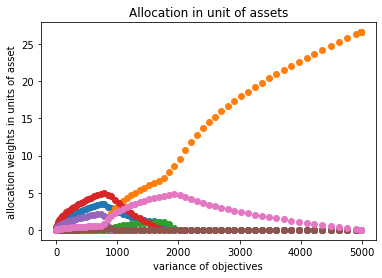
\includegraphics[width=0.9\linewidth,height =0.7\linewidth, angle=0]{single perid allocation units.png}
        \caption{Allocation weights in units of asset(Single Period)}
         \label{fig:single perid allocation units}
\end{minipage}\hfill
\begin{minipage}{0.5\textwidth}
        \centering
        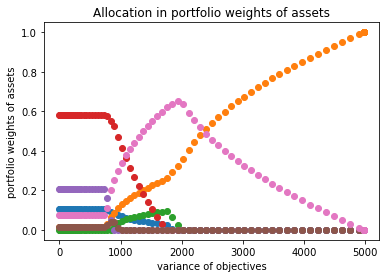
\includegraphics[width=0.9\linewidth,height =0.7\linewidth, angle=0]{single perid allocation weights.png}
        \caption{Allocation weights (Single Period)}
         \label{fig:single perid allocation weights}\end{minipage}
         \end{figure}


In the plot on the left, referenced as \cref{fig:single perid allocation units}, we illustrate the allocation weights in terms of asset units. On the other hand, in the plot on the right, referenced as \cref{fig:single perid allocation weights}, we present the allocation weights as relative portfolio weights.

It's clearly evident that as the allowed variance (risk) increases, the allocation on the efficient frontier tends to converge towards a corner solution. This outcome should be expected since we imposed additional constraints on the classical MVO framework (e.g. long-only). Such optimization problems often have a high likelihood of finding their maximizers/minimizers at the boundary.

\begin{figure}[!htp]
    \centering
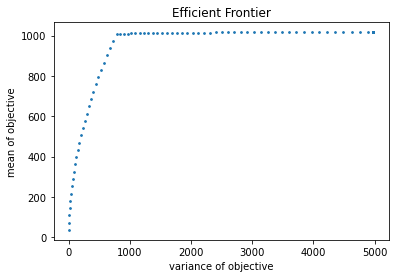
\includegraphics[width=0.5\textwidth]{single perid allocation efficient frontier.png}
    \caption{Single Period Allocation Efficient Frontier}
    \label{fig:single perid allocation efficient frontier}
\end{figure}
In \cref{fig:single perid allocation efficient frontier}, we display the risk/reward profile of the mean-variance efficient allocations in terms of expected value and variance of final wealth:
$$
\mathrm{E}\left\{\Psi_\alpha\right\}=\boldsymbol{\alpha}^{\top} \mathrm{E}\left\{\mathbf{P}_{T+\tau}\right\}, \quad \operatorname{Var}\left\{\Psi_{\boldsymbol{\alpha}}\right\}=\boldsymbol{\alpha}^{\top} \operatorname{Cov}\left\{\mathbf{P}_{T+\tau}\right\} \boldsymbol{\alpha} .
$$
It's easy to see that this efficient frontier looks different from the one we generated using fictional data in the section about classical MVO. This is because the various constraints we impose on the optimization process distort the behavior of the optimal allocation, resulting in a steep increase at first which then becomes flat afterwards.

{\color{C6}\textbf{Analysis 2: APT Model}}

Here, we analyze the four risk factors as stated in \cref{item:Black-Litterman-APT} estimated over the full scale dataset from $2012-01-09$ to $2017-01-02$.

\begin{figure}[!htp]
    \centering
    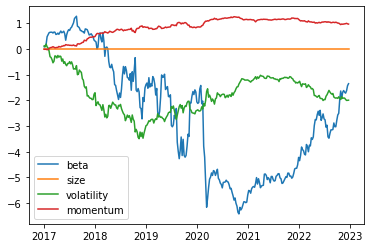
\includegraphics[width=0.5\textwidth]{apt.png}
    \caption{Cumulative factor returns to risk premia $\hat{\boldsymbol{f}}_t$}
    \label{fig:apt}
\end{figure}

Since the APT model is essentially a linear model, whether the risk factors serve as positive or negative drivers depends solely on their associated coefficients in $\bm{f}$. The cumulative factor return is simply the cumulative sum of all $\hat{\boldsymbol{f}}_t$'s over a period of time. For each entry in the cumulative factor returns, if the plot shows a downward trend over time, it suggests that the most recent entries are turning negative. This indicates that there is a minus sign before the corresponding risk premia during that period, which implies that the risk premia serve as a negative driver for the stock price, and vice versa.

\cref{fig:apt} is consistent with our intuition. The cumulative factor returns to momentum risk premia (i.e. coefficients before the momentum risk premia) is consistently positive, meaning the sign before the momentum risk premia is mostly positive. This suggests that, in most cases, a stock with higher momentum tends to outperform one with lower momentum, after controlling for other systematic sources of risk. The cumulative factor returns to volatility risk premium is negative, meaning the sign before the volatility risk premia is mostly negative. This suggests that, in most cases, stocks with higher volatility tend to perform poorly after controlling for other systematic sources of risk. The size risk premium is flat, likely because all chosen stocks have very high market capitalization, rendering the influence of size negligible when comparing the performance of these selected stocks.

The weird shape of the market beta factor return actually makes sense. The downward trend of the market beta entry in the cumulative factor return during 2017-2019 suggests that the coefficients for market beta were negative most of the time during this period, implying that stocks correlating well with the market were punished. Since all our chosen stocks are from large companies, which usually correlate well with the market, most of them under-performed during this period. The drastic drop in the spring of 2020 due to COVID-19 could provide further evidence for this, as it indicates a big big negative sign before the market beta risk premium at the time. Even stocks with only slight correlation with the market were significantly, negatively impacted. However, at the end of 2020, as Biden started his rescue plan, the markets began to recover and the market beta entry in the cumulative factor return $\bm{f}$ started to increase. This suggests that the most recent coefficients (the market beta entries of the factor return $\bm{f}$) for market betas were turning positive, implying that stocks correlating well with the market were beginning to perform well. We can see from \cref{fig:stocks performance} and \cref{fig:market performance} below that it was indeed the case.

\begin{figure}[!htbp]
\begin{minipage}{0.5\textwidth}
        \centering
        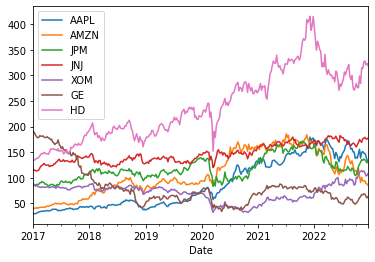
\includegraphics[width=0.9\linewidth,height =0.7\linewidth, angle=0]{stocks performance.png}
        \caption{Chosen stocks performance}
         \label{fig:stocks performance}
\end{minipage}\hfill
\begin{minipage}{0.5\textwidth}
        \centering
        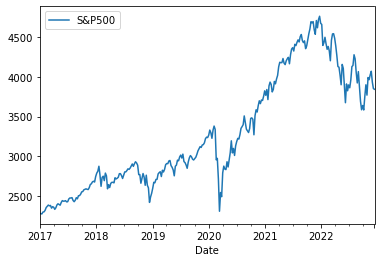
\includegraphics[width=0.9\linewidth,height =0.7\linewidth, angle=0]{market performance.png}
        \caption{Market performance}
         \label{fig:market performance}\end{minipage}
         \label{fig:stocks and marker performance}
         \end{figure}

\newpage
{\color{C6}\textbf{Analysis 3: Models Comparison}}

In this analysis, we compare the PnL curve of the five models that we purposed as shown in \cref{fig:five strategies}.
\begin{figure}
    \centering
    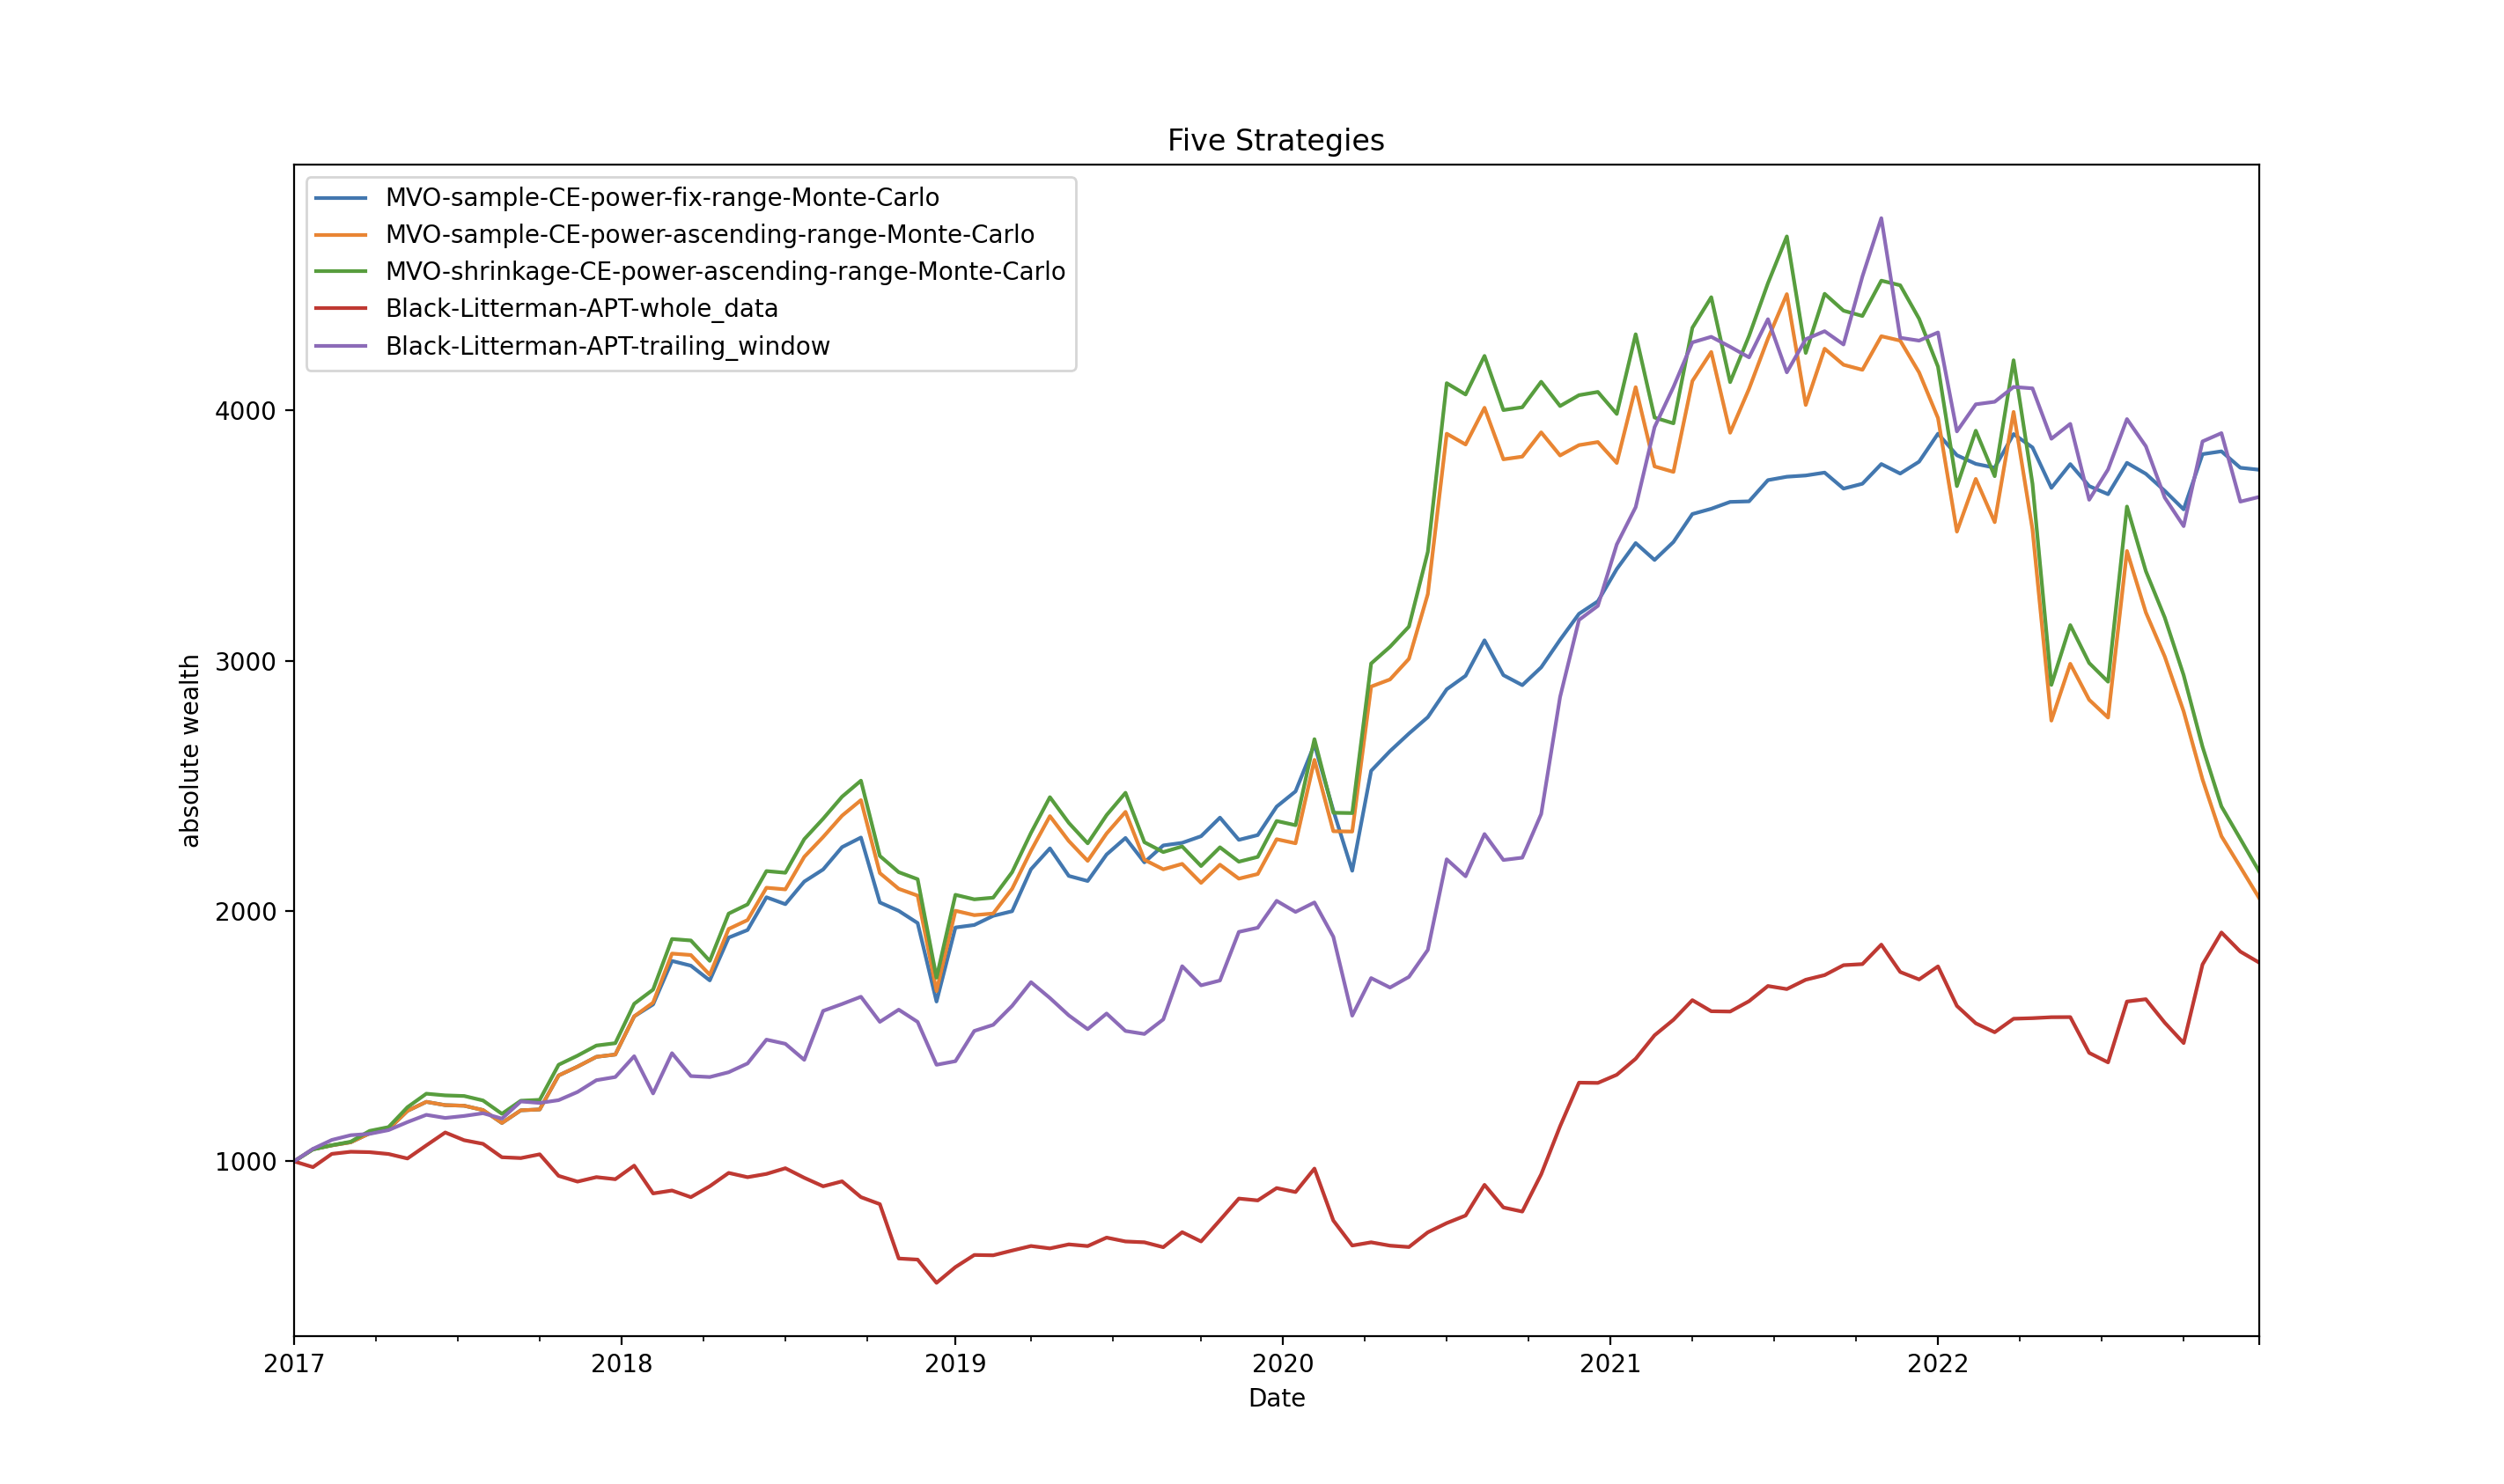
\includegraphics[width=1\textwidth]{five strategies.png}
    \caption{Performance of the five models proposed}
    \label{fig:five strategies}
\end{figure}
\begin{enumerate}
    \item \textbf{Finding 1: Shrinkage estimator perform better than vanilla sample estimator.}

    When comparing the performance of the model that uses the sample estimator with the one that uses the shrinkage estimator, it's easy to see that the shrinkage estimator outperforms the sample estimator consistently. This makes sense as the shrinkage estimator trades a bit more bias for less variance, resulting in a more robust and stable estimate. However, it's important to note that the impact of the estimators is relatively small. The most significant differences between the models still lie in the way they are constructed.
    \item \textbf{Finding 2: Maximizing certainty-equivalent does NOT mean maximizing absolute wealth.} 
    
    When comparing the performance of the MVO model with an increasing upper bound for the concerning variance to that of the MVO model with a fixed upper bound for the concerning variance, we observe that while the former generally outperforms the latter, it fails to maintain its lead towards the end. This suggests that optimal decisions guided by the certainty-equivalent index of satisfaction do not always guarantee superior performance. Essentially, this information implied by the index of satisfaction instructs you on how to make optimal investment decisions according to your risk preference.
    \item \textbf{Finding 3: Adjusting for economic understanding is essential.}

     When
comparing the performance of the Black-Litterman-APT model with estimations
conducted on a full-scale dataset — where the mean of the $\bm{f}$ -process is significantly influenced by data far removed from the time when the investor makes
their decision — and that of the Black-Litterman-APT model with estimations
based on a trailing 30-weeks window, it's apparent that the model that adjusts for
economic understanding, or what one might call data significance, performs far
better. This has led to the development of several practical techniques used by practitioners for data transformation, aiming to account for the greater reliability of more recent data compared to older data, such as exponential decay/smoothing.
    \item \textbf{Finding 4: Black-Litterman-APT model is not the holy grain.}

   Unlike the classical Black-Litterman model, which anchors its return to the market portfolio, the Black-Litterman-APT model does not anchor to anything. Alternatively, one could say its return is pegged on the inputs fed into the model. As in \textbf{Finding 3}, the performance of the Black-Litterman-APT model with estimations conducted on a full-scale dataset — where the mean of the $\bm{f}$-process is significantly influenced by data far removed from the time when the investor makes their decision — is way worse than that of the Black-Litterman-APT model with estimations based on a trailing 30-weeks window. This suggests that the performance of the Black-Litterman-APT model is dictated by how good your view $\bm{q}$ is and how good 
   your estimations are for the $\bm{f}$-process. However, the performance of the Black-Litterman-APT model is indeed much more stable.
\end{enumerate}







% \subsection{BL and the Cross-Sectional Momentum Strategy}

% \begin{itemize}
%   \item Combine cross-sectional momentum strategy with market equilibrium using the Black-Litterman model

%   \item One view: the momentum strategy

% \end{itemize}

% $\rightarrow \tau=0.1$

% \begin{itemize}
%   \item $\Omega$ derived from backtests (similar to $\left.\Omega=\operatorname{diag}\left(P \tau \mathbf{\Sigma} P^{\top}\right)\right)$

%   \item Standard MVO

%   \item Covariance matrices for the portfolio optimization are calculated from daily historical data with weighting (monthly decay parameter of $d=0.95)$ and with Newey-West correction for autocorrelation (2 lags) (Newey, West, et al., 1987)

%   \item Risk aversion $\lambda=2$ (calibrated to achieve about the same volatility as the index), monthly rebalancing

% \end{itemize}


% % \subsubsection{cross-sectional momentum strategy}
% % In this example, we developed a cross-sectional momentum strategy using daily returns of the individual constituents (developed market country indices) of the MSCI World Index over the period 1/1/1980 through 5/31/2004. The MSCI World Index is a free float-adjusted market capitalization index that is designed to measure global developed market equity performance. As of December 2004, the MSCI World Index consisted of the following 23 developed market country indices: Australia, Austria, Belgium, Canada, Denmark, Finland, France, Germany, Greece, Hong Kong, Ireland, Italy, Japan, the Netherlands, New Zealand, Norway, Portugal, Singapore, Spain, Sweden, Switzerland, the United Kingdom, and the United States. Other constituents that were part of the index at some point throughout the sample period were Malaysia, Mexico, and South African Gold Mines.


% % \begin{itemize}
% %   \item Data: Country indexes from the MSCI Developed Market Index

% %   \item Portfolio is constructed at a point in time $t$ and held for one month

% %   \item Sort countries based on their "one-day lagged" past nine month return normalized by their volatility

% % \end{itemize}

% % $$
% % z_{t, i}=\frac{P_{t-1 \text { day }, i}-P_{t-1 \text { day }-9 \text { months }, i}}{P_{t-1 \text { day }-9 \text { months }, i} \cdot \sigma_{i}}
% $$

% \begin{itemize}
%   \item Long-short portfolio:

%   \item Countries in the top half are assigned a weight of $w_{i}=\frac{1}{\sigma_{i} \cdot \kappa}(\kappa$ is a scaling factor such that annual portfolio volatility is around $20 \%)$

% \end{itemize}

% \begin{itemize}
%   \item Countries in the bottom half are assigned a weight of $w_{i}=-\frac{1}{\sigma_{i} \cdot \kappa}$

%   \item Note that this is not a zero cost long-short portfolio as the portfolio weights do not sum up to zero

% \end{itemize}
% Remarks
% \begin{itemize}
%   \item In the figures about we examined the cross-sectional momentum strategy. There is no MVO here

%   \item We did not do any tweaking: simple and straightforward "textbook" cross-sectional momentum strategy

%   \item The Sharpe ratio of the strategy over the full period is 0.88 versus 0.62 for the index

%   \item The full period annualized alpha is $11.7 \%$; beta is only 0.05 for the full sample (market neutral). Realized correlation between the momentum strategy and the index is $3.5 \%$

%   \item Average monthly portfolio turnover of $23.7 \%$ with a cross-sectional standard deviation of $9.3 \%$. United Kingdom has the highest average turnover $(40.6 \%)$, and New Zealand has the lowest $(10.8 \%)$

% \end{itemize}

% \begin{remark}\hfill 
%     \begin{enumerate}
%   \item We did not do any tweaking: simple and straightforward "textbook" cross-sectional momentum strategy

%   \item B-L strategy has a full sample Sharpe ratio of 0.92 versus 0.62 for the index and an "alpha" of 8.3\%.

%   \item Full sample correlation between the strategy and the index is 0.36 (no beta constraints)

%     \end{enumerate}
% \end{remark}



% \newpage
%%%%%%%%%%%%%%%%%%%%%%%%%%%%%



% \subsection{PRACTICAL CONSIDERATIONS WHEN USING BLB MODELS}
% In this section, we address the key aspects that are important to any implementation of the BL and BLB models: (1) choice of prior, (2) view generation, and (3) transaction costs.

% \newpage
% %%%%%%%%%%%%%%%%%%%%%%%%%%%%%%%%%%%%%%%%%%%%%%%%%
% \section{Robust Optimization}
% Recently, robust optimization techniques, originally developed in the area of operations research and optimization theory, have received significant interest by the investment management community. These techniques allow the portfolio manager to incorporate estimation errors directly into the portfolio optimization. In a nutshell, standard optimizers take inputs as given with complete certainty, where as robust optimizers incorporate the uncertainty introduced by estimation error directly into the optimization process.4 Improved estimation techniques, such as the Black-Litterman model, can be effectively applied in combination with robust portfolio optimization.

% We next describe the application of so-called robust optimization methods to the BL model. Robust approaches to optimization are designed to mitigate the impact of model misspecification on portfolio construction.






\newpage
\section{Future Work: MVO with transaction cost}
The traditional Mean-Variance Optimization (MVO) approach often results in portfolio allocations that incur substantial trading costs, significantly impacting realized risk-adjusted returns. As demonstrated in the empirical example, we incorporated transaction costs into the classical MVO framework; however, this model is simplified and does not fully capture the complexities of reality.

In the real world, transaction costs include direct costs such as commissions and taxes, the bid-ask spread, and indirect costs like slippage and market impact. Slippage is defined as the price difference between the time a trade is anticipated and the volume-weighted average price at which it executes. Market impact refers to the price changes caused by the trade itself, which can be substantial when the size-to-average volume ratio of trades is high.

Fortunately, several models have been proposed in the literature to address these issues, such as those by Hasbrouck (1991), Lillo, Farmer, and Mantegna (2003), and Almgren, Thum, Hauptmann, and Li (2005). Consequently, in future research, we could consider incorporating their ideas into our framework.
% \subsection{MVO with additional constraints}

% \subsection{risk-parity portfolios}
% \subsection{the problem of mixing different sources of alpha}

\newpage
\section{Appendix}
\subsection{Von Neumann-Morgenstern Utility Theory}
In decision theory, {\color{C3}the von Neumann–Morgenstern (VNM) utility theorem shows that any individual whose preferences satisfied four VNM axioms has a utility function (VNM Theorem); such an individual's preferences can be represented by $U(\mathbf{p})$}, the von Neumann–Morgenstern utility function.  {\color{C2}And the individual will always prefer actions that maximize expected utility (Expected Utility Hypothesis).}  The theorem is the basis for expected utility theory.

\subsubsection{VNM -- Formulate the Question}
VNM start with Knightian Risk (finite probability space) and assumed:
\begin{enumerate}[label=(\arabic*)]
    \item \textbf{Outcomes: } mutually exclusive outcomes $(s_1, s_2, \dots, s_n)$.

    \textbf{E.g. } Toss of a coin -- two possible outcomes; heads ($s_1$) or tails ($s_2$). 
    \item \textbf{Prizes: } The monetary amounts that each outcome maps to.
    \item \textbf{Lottery:} A scenario where a set of probabilities (Probability Vector) $\mathbf{p} = (p_1, p_2, \dots, p_n)$ is assigned to the outcomes $(s_1, s_2, \dots, s_n)$. 
    \item \textbf{Lottery Set:} Define $\Delta(s)$ as the set of all lotteries on $s$; that is, the set of all probability vectors $\mathbf{p} \in \mathbb{R}^n$.

    Clearly $\Delta(s)$ is convex; if $p_1, p_2\in\Delta(s)$, then for any $0\leq\alpha\leq1$, $\alpha p_1+(1-\alpha)p_2\in\Delta(s)$ must hold.
    \item \textbf{Preference Function:} A ranking between lotteries in $\Delta(s)$ is a binary relation $\succeq$. 
    \begin{enumerate}[label=(\alph*)]
        \item For two lotteries $\mathbf{p},\mathbf{q}\in\Delta(s)$ we write $\mathbf{p}\succeq \mathbf{q}$ if $\mathbf{p}$ is preferred to or equivalent to $\mathbf{q}$.
        \item Equivalence is denoted by $\equiv$ and means both $\mathbf{p}\succeq \mathbf{q}$ and $\mathbf{q}\succeq \mathbf{p}$.
        \item $\mathbf{p}\succ \mathbf{q}$ means strictly preferred.
    \end{enumerate}
    \item Economic agent ranks lotteries (probability vectors).
\end{enumerate}

\begin{point}
    \textbf{Example: } $3$ outcomes $\longrightarrow$  $3$ prizes:
    $$
    \begin{aligned}
    & \mathrm{s}_{1}=\text { you receive } \$ 0 \\
    & \mathrm{s}_{2}=\text { you receive } \$ 500,000,000 \\
    & \mathrm{s}_{3}=\text { you receive } \$ 1,000,000,000
    \end{aligned}
    $$

People decide between lotteries $\mathbf{p}_{1}=(0,1,0)$ and $\mathbf{p}_{2}=(.5,0, .5)$.
\end{point} 

\subsubsection{VNM Axioms}

\begin{enumerate}[label=(\arabic*)]
  \item \textbf{Transitivity: } For $\mathbf{p}, \mathbf{q}, \mathbf{r} \in \Delta(s), \mathbf{p} \succeq \mathbf{q}$ and $\mathbf{q} \succeq \mathbf{r}$ means $\mathbf{p} \succeq \mathbf{r}$.

  $\Longrightarrow$ No circular preferences: if I like chocolate better than vanilla and vanilla better than strawberry, then I like chocolate better than strawberry.
  \item \textbf{Completeness: } For $\mathbf{p}, \mathbf{q} \in \Delta(s)$, either $\mathbf{p} \succeq \mathbf{q}$ or $\mathbf{q} \succeq \mathbf{p}$ or both. If both are true then we say $\mathbf{p} \equiv \mathbf{q}$.

  $\Longrightarrow$ Only one view.
  
  $\Longrightarrow$ Can be lotteries that are not the same but are equivalent.
  
  $\Longrightarrow$ \textbf{Reflexivity: } $(\mathbf{p} \succeq \mathbf{p}$ so $\mathbf{p} \equiv \mathbf{p})$ follows from Completeness.
  \item \textbf{Independence: } If $\mathbf{p}, \mathbf{q}, \mathbf{r} \in \Delta(s)$ with $\mathbf{p} \succeq \mathbf{q}$ and $\alpha \in[0,1]$, then $\alpha \mathbf{p}+(1-\alpha) \mathbf{r} \succeq \alpha \mathbf{q}+(1-\alpha) \mathbf{r}$.

  $\Longrightarrow$ If I like chocolate better than strawberry, then I like (a mixture of chocolate and vanilla) better than (the same mixture of strawberry and vanilla).

  $\Longrightarrow$ \textbf{Strong/Debatable Axiom}: there could be interactions between items that would alter the results.
  \item \textbf{Continuity: } If $\mathbf{p}, \mathbf{q}, \mathbf{r} \in \Delta(s)$ with $\mathbf{p} \succeq \mathbf{q} \succeq \mathbf{r}$, then there is a scalar $\alpha \in[0,1]$ such that $\alpha \mathbf{p}+(1-\alpha) \mathbf{r}=\mathbf{q}$.

  $\Longrightarrow$ If I prefer chocolate to vanilla, and I prefer vanilla to strawberry, then there is some mixture of chocolate and strawberry that I like the same as vanilla.

  $\Longrightarrow$ \textbf{Strong/Debatable Axiom}: I might hate the taste of mixtures and dislike even the smallest adulteration of my beloved chocolate, so there is no combination that gets me to the same satisfaction level as vanilla.
\end{enumerate}

\begin{remark}
    Eventually these axioms go bad - people don't actually behave like this if we push it far enough. 
\end{remark}

\subsubsection{VNM Theorem}
VNM Theorem quantified the more intuitive preference functions by showing that 
\[
\text{utility functions}\quad = \quad \text{preference functions}.
\]
\begin{theorem}\textbf{(VNM Theorem)} let $\Delta(s)$ be a convex subset of ${\mathbb{R}^n}$. Let $\succeq$ be a binary relation on $\Delta(s)$. Then $\succeq$ satisfies the four VNM axioms if and only if there is a function $U:\Delta(s)\rightarrow\mathbb{R}$ such that:
\begin{enumerate}[label=(\alph*)]
    \item U represents $\succeq$.  (i.e. $\forall \mathbf{p}, \mathbf{q}\in\Delta(s)$, $\mathbf{p}\succeq \mathbf{q} \iff U(\mathbf{p})\geq U(\mathbf{q})$)
    \item $U$ is affine. (i.e. $\forall \mathbf{p},\mathbf{q}\in\Delta(s), \alpha\in[0, 1]$, $U(\alpha \mathbf{p} + (1- \alpha)\mathbf{q}) = \alpha U(\mathbf{p}) + (1- \alpha)U(\mathbf{q})$)
\end{enumerate}
\end{theorem}

\begin{solution}
Set elementary lotteries $\mathbf{x}_i = \mathbf{e}_i$ where the $i^{th}$ outcome $s_i$ has $100\%$ probability of happening. Suppose $\mathbf{x}_n\succeq \mathbf{x}_{n-1}\succeq \dots \succeq \mathbf{x}_1$. Start construction of the utility function $U$ by defining $U(\mathbf{x}_1)=u(s_1)=0$ and $U(\mathbf{x}_n)=u(s_n)=1$, unless $x_n\equiv x_1$ in which case the trivial utility function $U(\mathbf{x})=0$ for all lotteries $\mathbf{x}$. 

By the continuity axiom, there is an $\alpha_i$ so that $\alpha_i \mathbf{x}_n + (1-\alpha_i)\mathbf{x}_1\equiv x_i$ for any $1\leq i \leq n$. Then set $U(\mathbf{x}_i)=u(s_i) =\alpha_i$. Then, for any lottery $\mathbf{p}=(p_1,\dots,p_n) = \sum_{i=1}^n \mathbf{x}_i p_i$, we have
    \begin{align*}
        U(\mathbf{p}) &= p_1U(\mathbf{x}_1)+p_2U(\mathbf{x}_2)+\cdots + p_nU(\mathbf{x}_n)\\
        &=p_1u(s_1)+p_2u(s_2)+\cdots + p_nu(s_n)
    \end{align*}
where $u$ assigns to each outcome $s_i$ a real number $u(s_i)$.

This construction makes sense because for any lottery $\mathbf{p}$ \begin{align*}
        \mathbf{p}=(p_1,\dots,p_n) &= \sum_{i=1}^n \mathbf{x}_i p_i\\
        &\equiv \sum_{i=1}^n (\alpha_i \mathbf{x}_n + (1-\alpha_i)\mathbf{x}_1) p_i\\
        &=\left(\sum_{i=1}^n \alpha_i p_i\right) \mathbf{x}_n + \left(1-\sum_{i=1}^n \alpha_i p_i\right)\mathbf{x}_1\\
        &=U(\mathbf{p})\mathbf{x}_n+(1-U(\mathbf{p}))\mathbf{x}_1
    \end{align*}

    That is, lottery $\mathbf{p}=(p_1,\dots,p_n)\equiv(1-U(\mathbf{p}),0,\dots,0,U(\mathbf{p}))$. 
    
    It follows that
\begin{align*}&\mathbf{p}\succeq \mathbf{q}\\
\Longleftrightarrow &(1-U(\mathbf{p}),0,\dots,0,U(\mathbf{p}))\succeq (1-U(\mathbf{q}),0,\dots,0,U(\mathbf{q}))\\
\text{By Lemma}\Longleftrightarrow &U(\mathbf{p}) \ge U(\mathbf{q})
    \end{align*}
    which is consistent with our aim of construction. Also, $U(\mathbf{p})$ is apparently affine.
\end{solution}

\begin{remark}\hfill
\begin{enumerate}
    \item Utility Functions are here to help us rank lotteries, so there is no true meaning of them. 
    \item $U$ is unique up to a positive linear transformation: If $V:\Delta(s)\rightarrow\mathbb{R}$ also satisfies (a) and (b), then there are $b,c\in\mathbb{R}$ (where $b > 0$) such that $V = bU + c$.
    \item {\color{C3}Normally, we will use this theorem in the reverse order by directly saying a person's utility function is xxx so that we have a preference relation.}
    \item $U(\mathbf{p})$ is called the VNM utility functions, and $u(s_i)$ is called the Bernoulli utility functions.
    \item \textbf{Non-Satiation: } All else being constant, individuals always prefer more of positive goods rather than negative goods, vice versa. Therefore, we have $u^{\top}(x) \geq 0$.
\end{enumerate}
\end{remark}


\begin{theorem}\textbf{(Expected Utility Hypothesis)}  An individual chooses not the highest expected value, but rather the highest expected utility; that is one would want to maximize
\begin{align*}
        U(\mathbf{p}) &= p_1U(\mathbf{x}_1)+p_2U(\mathbf{x}_2)+\cdots + p_nU(\mathbf{x}_n)\\
        &=p_1u(s_1)+p_2u(s_2)+\cdots + p_nu(s_n)
    \end{align*}
\end{theorem}



\begin{definition}\textbf{(Certainty Equivalent)} Given a utility function on prizes and a lottery $\mathbf{p}$, the certainty equivalent of $\mathbf{p}$ is the number $m$ such that
\[ u(m)=\EE_{\mathbf{p}}[u(X)]
\]
where $m$ is sure prize that has the same utility as risky outcomes encoded in $X$ with probabilities in $\mathbf{p}$. 
\end{definition}

\subsubsection{Problems with utility theory}
Why? 1.the overstrong set of assumptions about what constitutes rational decision making, 2. humans are irrational.


\begin{problem}\textbf{(The Allais Paradox)}\hfill
\begin{enumerate}[label=(\arabic*)]
    \item Decision 1: Choose between two lotteries. $\mathbf{p}_{1}$ gives a $63 \%$ chance of $\$ 500,000 \cdot \mathbf{p}_{2}$ gives a $61 \%$ chance of $\$ 520,000$.
    \item Decision 2: Choose between two lotteries. $\mathbf{q}_{1}$ gives a $100 \%$ chance of $\$ 500,000 . \mathbf{q}_{2}$ gives a $98 \%$ chance of $\$ 520,000$.
\end{enumerate}
Should be clear that $\mathbf{p}_{2}, \mathbf{q}_{1}$ (which is fairly common) violates utility theory.

\begin{solution}
    Most people choose 1a and 2b. But if 1a is preferred to 1b, we must have
$$.61u(520)+.39u(0)>.63u(500)+.37u(0)$$
where u(x) means the utility of gaining x thousand dollars. Thus
$$.61(u(520)-u(500))>.02(u(500)-u(0))$$
Assuming only that the utility function $u$ is sensible (more is preferred to less, $u^{\top}>0$), both sides of this last inequality are positive.

Preferring the certain 2b to the highly probable 2a means
$$u(500)>.98u(520)+.02u(0)>0$$
which gives
$$.02(u(500)-u(0))>.98(u(520)-u(500))$$
Thus for any sensible utility function, $1a\succ 1b$ and $2b\succ 2a$ are incompatible.
\end{solution}
\end{problem}

{\color{C3}Conclusion:} We will see various laws indicating that relying on any mathematical finance or economics "law" too heavily will break. The point of financial and economic modeling is to inform human intuition, not (yet) to replace it. Utility remains a powerful concept and a good first-order guide to economic decision-making. 
% \subsubsection{Formalization}

% \subsection{practical
% multi-period portfolio optimization}
% Multi-period extensions of MVO to incorporate intertempo-
% ral effects such as hedging needs, changing market condi-
% tions, market impact costs, and alpha decay

\newpage
\begin{thebibliography}{9}

\bibitem{meucci2009} 
Meucci, A. 
\textit{Risk and asset allocation}. 
Springer Science \& Business Media, 2009.

\bibitem{black1991} 
Black, F., \& Litterman, R. B. 
\textit{The Journal of Fixed Income}, 1(2), 7-18. 
https://doi.org/10.3905/jfi.1991.408013, 1991.

\bibitem{luenberger1998} 
Luenberger, D. G. 
\textit{Investment Science}. 
New York: Oxford University Press, 1998.


\bibitem{henderson1981} 
Henderson, H. V., \& Searle, S. R. 
\textit{On Deriving the Inverse of a Sum of Matrices}. 
SIAM Review, 23(1), 53–60. 
https://doi.org/10.1137/1023004, 1981.

\bibitem{he} 
He, G., \& Litterman, R. 
\textit{The Intuition Behind Black-Litterman Model Portfolios}. 
Available at SSRN: https://ssrn.com/abstract=334304 or http://dx.doi.org/10.2139/ssrn.334304.

\bibitem{kolm2008} 
Kolm, P. N., Focardi, S. M., \& Fabozzi, F. J. 
\textit{Incorporating Trading Strategies in the Black-Litterman Framework}. 
In F. J. Fabozzi (Ed.), Handbook of Finance. 
https://doi.org/10.1002/9780470404324.hof002036, 2008.

\bibitem{ritter2016} 
Ritter, G. 
\textit{Stable Linear-Time Optimization in Arbitrage Pricing Theory Models}. 
Risk Magazine. Available at SSRN: https://ssrn.com/abstract=2821360, 2016.

\bibitem{kolm2017} 
Kolm, P., \& Ritter, G. 
\textit{On the Bayesian Interpretation of Black–Litterman}. 
European Journal of Operational Research, 258(2), 564–72. 
https://doi.org/10.1016/j.ejor.2016.10.027, 2017.

\bibitem{theil_goldberger_1961} 
Theil, H. and Goldberger, A. S.
\textit{On pure and mixed statistical estimation in econometrics},
International Economic Review, vol. 2, no. 2, pp. 65--78, 1961.

\end{thebibliography}


\end{document}
